% !TEX root = main.tex
\documentclass[openany]{book}
    \usepackage[acronym]{glossaries}
    \usepackage[english]{babel}
    \usepackage{lipsum}
    \usepackage{hyperref}
    \usepackage{booktabs}
    \usepackage[utf8]{inputenc}
    \usepackage[a4paper,margin=2.5cm]{geometry}%2.5cm
    \usepackage{algorithm}
    \usepackage{algpseudocode}
    \usepackage{multirow}
    \usepackage{setspace}
    \usepackage[parfill]{parskip}
    \usepackage{graphicx}
    \usepackage[margin=1cm,font=normalsize,labelfont=bf]{caption}
    \usepackage{placeins}
    \usepackage{csquotes} 
    \usepackage{listings,xcolor}
    \usepackage[most]{tcolorbox}     
    \usepackage{pgfplots}
    \usepackage{tikz}
    \usepackage[
    backend=biber,
    style=numeric,
]{biblatex}

\usetikzlibrary{arrows.meta,positioning,fit,backgrounds,shapes.misc}

\addbibresource{refs.bib}

\newtcolorbox{myquote}{
    enhanced,
    frame hidden,
    colback=gray!10,
    sharp corners,
    left=10pt,
    right=0pt,
    borderline west={2pt}{0pt}{gray!50}
}

\newcommand{\CaptionFontSize}{\small}
\newcommand{\mdblockquote}[1]{  \begin{myquote}  #1  \end{myquote}  }

\makeglossaries
\newacronym{ui}{UI}{User Interface}
\newacronym{ux}{UX}{User Experience}
\newacronym{ai}{AI}{Artificial Intelligence}
\newacronym{ml}{ML}{Machine Learning}
\newacronym{hci}{HCI}{Human-Computer Interaction}
\newacronym{gui}{GUI}{Graphical User Interface}
\newacronym{llm}{LLM}{Large Language Model}
\newacronym{nlp}{NLP}{Natural Language Processing}
\newacronym{api}{API}{Application Programming Interface}
\newacronym{vr}{VR}{Virtual Reality}
\newacronym{xr}{XR}{Extended Reality}
\newacronym{ar}{AR}{Augmented Reality}
\newacronym{vlm}{VLM}{Vision-Language Model}
\newacronym{react}{ReAct}{Reasoning and Acting}
\newacronym{rpa}{RPA}{Robotic Process Automation}
\newacronym{nlpui}{NLP UI}{Natural Language Processing User Interface}
\newacronym{dsl}{DSL}{Domain-Specific Language}
\newacronym{tui}{TUI}{Tangible User Interface}
\newacronym{cli}{CLI}{Command-Line Interface}
\newacronym{ide}{IDE}{Integrated Development Environment}
\newacronym{pbd}{PBD}{Programming by Demonstration}
\newacronym{vpl}{VPL}{Visual Programming Language}
\newacronym{cot}{CoT}{Chain of Thought}
\newacronym{seeact}{SeeAct}{Seeing and Acting}
\newacronym{autogpt}{AutoGPT}{Autonomous GPT}
\newacronym{gpt}{GPT}{Generative Pre-trained Transformer}

\definecolor{background}{HTML}{EEEEEE}

\lstdefinelanguage{json}{
    basicstyle=\normalfont\ttfamily,
    numbers=left,
    numberstyle=\scriptsize,
    breaklines=true,
    frame=lines,
    backgroundcolor=\color{gray!10},
    showstringspaces=false,
    string=[db]{"},
    stringstyle=\color{green!50!black},
    morestring=[s][\color{black}]{\ \ "}{":},
    keywordstyle=\color{blue},
    keywords={true,false,null},
    literate=
     *{0}{{{\color{red}0}}}{1}
      {1}{{{\color{red}1}}}{1}
      {2}{{{\color{red}2}}}{1}
      {3}{{{\color{red}3}}}{1}
      {4}{{{\color{red}4}}}{1}
      {5}{{{\color{red}5}}}{1}
      {6}{{{\color{red}6}}}{1}
      {7}{{{\color{red}7}}}{1}
      {8}{{{\color{red}8}}}{1}
      {9}{{{\color{red}9}}}{1}
      {.}{{{\color{red}.}}}{1}
      {:}{{{\color{gray}{:}}}}{1}
      {,}{{{\color{gray}{,}}}}{1}
      {\{}{{{\color{gray}{\{}}}}{1}
      {\}}{{{\color{gray}{\}}}}}{1}
      {[}{{{\color{gray}{[}}}}{1}
      {]}{{{\color{gray}{]}}}}{1},
}

\lstdefinelanguage{Dart}{
    morekeywords={
        abstract, as, assert, async, await, break, case, catch, class, const, continue,
        covariant, default, deferred, do, dynamic, else, enum, export, extends, extension,
        external, factory, false, final, finally, for, Function, get, hide, if, implements,
        import, in, inferface, is, late, library, mixin, new, null, on, operator, part,
        rethrow, return, set, show, static, super, switch, sync, this, throw, true, try,
        typedef, var, void, while, with, yield
    },
    sensitive=true,
    morecomment=[l]{//},
    morecomment=[s]{/*}{*/},
    morestring=[b]",
    morestring=[b]',
    stringstyle=\color{green!50!black},
    keywordstyle=\color{blue}\bfseries,
    commentstyle=\color{gray}\itshape,
    basicstyle=\ttfamily\small,
    numbers=left,
    numberstyle=\scriptsize,
    breaklines=true,
    frame=lines,
    backgroundcolor=\color{gray!10},
    showstringspaces=false,
}


\begin{document}

\begin{titlepage}

\newcommand{\HRule}{\rule{\linewidth}{0.5mm}} % Defines a new command for the horizontal lines, change thickness here

\center
 
%----------------------------------------------------------------------------------------
%	HEADING SECTIONS
%----------------------------------------------------------------------------------------

\textsc{\LARGE Hasselt University}\\[1.0cm]
\textsc{\Large Master's thesis presented for the attainment of the degree of Master of Science in Computer Science}\\[0.5cm]

%----------------------------------------------------------------------------------------
%	TITLE SECTION
%----------------------------------------------------------------------------------------
\HRule \\[0.2cm]
{ \huge  \bfseries A Multimodal AI-Driven GUI Framework for Dynamic User Adaptation \par} 
\HRule \\[1.5cm]
 
%----------------------------------------------------------------------------------------
%	AUTHOR SECTION
%----------------------------------------------------------------------------------------

\begin{minipage}[t]{0.5\textwidth}
    \begin{flushleft}
        \large \textit{Author}:\vspace*{0.5cm} \\
        Yarne Dirkx
    \end{flushleft}
\end{minipage}%
%
\begin{minipage}[t]{0.5\textwidth}
    \begin{flushright}
        \large \textit{Promotor}:\vspace*{0.5cm} \\
        Prof. Dr. Kris Luyten\\
        \vspace*{0.5cm}
    \end{flushright}
\end{minipage}

\vspace*{1cm}

%----------------------------------------------------------------------------------------
%	DATE SECTION
%----------------------------------------------------------------------------------------

{\large Academic year 2024-2025}\\[2cm]

%----------------------------------------------------------------------------------------
%	LOGO SECTION
%----------------------------------------------------------------------------------------


\includegraphics[width=0.4\textwidth]{images/uhasselt.jpg}\\
 
%----------------------------------------------------------------------------------------

\vfill % Fill the rest of the page with whitespace

\end{titlepage}

\chapter*{Abstract}
This thesis presents a multimodal AI-driven GUI framework for dynamic user interface adaptation, enabling real-time, personalised accessibility enhancements across platforms such as Flutter, SwiftUI, and beyond. Designed with a focus on the health domain, the framework supports motor-impaired, visually impaired, and hands-free users by integrating diverse input modalities including touch, keyboard, voice, and gestures.
At its core is Smart Intent Fusion (SIF), a multi-agent architecture powered by large language models (LLMs) via the Google Gemini API. SIF fuses user inputs, events, profiles, and interaction history to infer intent and propose targeted UI adaptations such as button enlargement, contrast enhancement, and navigation mode switching. The SIF reasoning engine combines rule-based logic for predictable, low-latency responses with LLM-driven reasoning for complex or ambiguous cases.
The framework provides developer-friendly integration through standardised JSON contracts and a FastAPI backend, making it portable across domains and platforms. Its feasibility was evaluated using six diverse user profiles, each representing different accessibility needs. For each profile, two sequential runs of seven multimodal interaction events were executed, allowing the system to adapt both to immediate interaction errors (e.g., miss-taps, slider overshoots) and to evolving user histories. Configurations were assessed for schema validity, action alignment with profile needs, and latency distribution, supported by per-profile breakdowns and global action analysis. This study demonstrated that the system consistently produced accessibility-targeted adaptations, with measurable strengths and areas for refinement in personalisation and latency handling.
By addressing the gap in intelligent, multimodal UI adaptation, this work helps advance human-computer interaction and lays the foundation for future AI models capable of autonomously rewriting UI code, offering a scalable and extensible solution for personalised user experiences.

\chapter*{Acknowledgments}
I would like to express my deepest appreciation to all those who have supported and guided me throughout the course of my master’s thesis.

First and foremost, I am sincerely grateful to Prof. Dr. Kris Luyten, my thesis supervisor, for his invaluable guidance, constructive feedback, practical tips, and continuous support.

My heartfelt gratitude extends to my family, especially my sister Phaedra, my brother-in-law Dennis, and my parents for their unwavering support, patience, and help with proofreading.

I would also like to thank my fellow students for their encouragement, collaboration, and support during this journey. Special thanks go to my two dogs, Tobias and Casper, whose company during countless late-night coding sessions, and gentle reminders to take breaks helped keep me grounded.

Finally, I am thankful to my friends for their motivation, belief in my abilities, and for making this challenging journey a rewarding one.

This work would not have been possible without the contribution and support of all these people, to whom I am deeply grateful.

\chapter*{Nederlandse Samenvatting}
\section*{Inleiding}
Grafische gebruikersinterfaces (GUI's) vormen de kern van hoe we dagelijks met technologie omgaan, van smartphones tot websites en smartwatches. Deze interfaces maken complexe taken toegankelijk door visuele elementen zoals knoppen, iconen en menu's te gebruiken, in plaats van tekstgebaseerde commando's. Vóór de opkomst van GUI's in de jaren 1980 waren command-line interfaces (CLI's) dominant, wat computing beperkte tot experts die commando's moesten memoriseren. GUI's hebben dit veranderd door visuele metaforen te introduceren, waardoor technologie beschikbaar werd voor het brede publiek. Ze vertalen ingewikkelde computertaken naar intuïtieve, visuele acties.

In de loop der jaren zijn GUI's geëvolueerd van het klassieke WIMP-model (windows, icons, menus, pointers) naar multimodale systemen die touch, stem, gebaren en zelfs ruimtelijke interacties in augmented reality (AR) en virtual reality (VR) omvatten. Dit biedt rijkere en natuurlijkere interacties. Toch blijven de meeste GUI's statisch: ze volgen een one-size-fits-all aanpak, met dezelfde lay-out, gedrag en visuele elementen voor alle gebruikers, ongeacht hun behoeften of context. Dit creëert barrières in een diverse wereld, vooral voor gebruikers met toegankelijkheidsuitdagingen. Mensen met visuele beperkingen worstelen met laag contrast of gebrek aan screenreader-ondersteuning, terwijl motorisch beperkte gebruikers moeite hebben met kleine knoppen of precieze taps. Handsfree gebruikers, zoals in medische contexten, hebben alternatieve invoermethoden nodig.

Gebruikers interacteren bovendien in variërende omgevingen – lawaaierig, felverlicht of onderweg – wat interactie verder compliceert. Apparaten variëren in grootte en capaciteit, van smartwatches tot desktops, maar toegankelijkheidsfuncties zijn vaak inconsistent. Dit benadrukt een kernuitdaging: hoe ontwerpen we GUI's die dynamisch aanpassen aan individuele toegankelijkheidsbehoeften en context, voor inclusieve en efficiënte interactie?

Adaptieve gebruikersinterfaces (UI's) passen zich dynamisch aan aan gebruikersbehoeften en contextuele factoren. Ze wijzigen lay-out, gedrag of uiterlijk op basis van voorkeuren, vaardigheden en omstandigheden. Door multimodale invoer zoals touch, stem, gebaren en gaze te verwerken, bieden ze gepersonaliseerde, inclusieve ervaringen, vooral voor diverse gebruikersgroepen. Een 'intelligente' interface interpreteert complexe gedragingen autonoom en leert van interacties in real-time. Kunstmatige intelligentie (AI), inclusief machine learning en grote taalmodellen (LLM's), maakt dit mogelijk door invoer, UI-context en gebruikersdata te verwerken.

LLM's zoals GPT hebben natuurlijke taalverwerking gerevolutioneerd. Ze begrijpen context, leiden intentie af en genereren menselijke reacties, ideaal voor multimodale interpretatie. In adaptieve UI's fungeren LLM's als controllers die interacties vertalen naar aanpassingen, zoals het vergroten van knoppen op basis van een stemcommando of aarzeling in gebaren. Ze kunnen zelfs UI-elementen genereren door de interface als API te behandelen.

Ondanks onderzoek en technologie blijven adaptieve UI's zeldzaam door implementatiecomplexiteit en gebrek aan frameworks. Dit motiveerde deze scriptie, geïnspireerd op ideeën om UI's als API's te behandelen, bestuurd door intelligente modellen. LLM's bieden potentieel, maar hebben uitdagingen zoals latency, hallucinaties en gebrek aan specialisatie voor GUI-taken. Deze scriptie ziet LLM's als contextbewuste assistenten die, met begeleiding, UI-aanpassingen verbeteren.
\newpage
\textbf{Probleemstelling en Onderzoeksdoelen}

De meeste applicaties zijn statisch en passen zich niet aan aan veranderende contexten of beperkingen. Huidige adaptaties zijn cosmetisch, zoals aanpassing aan schermgrootte, maar pakken niet de diepere uitdagingen aan van intentie, cognitieve staat of fysieke limieten in real-time.
Het ontwerpen van adaptieve UI's is ongewoon door technische moeilijkheden in modellering en gebrek aan frameworks. Real-world interactie is chaotisch: kleine variaties zoals een miss-tap of omgevingsruis leiden tot divergenties, wat regelgebaseerd ontwerp fragiel maakt.

Dit vereist systemen die nuances interpreteren, geschikt voor AI zoals LLM's. Bestaande frameworks integreren zulke modellen zelden voor real-time adaptatie, wat een kloof creëert tussen potentieel en praktijk.
Het primaire doel is een modulair, multimodaal AI-framework te ontwerpen, implementeren en valideren voor dynamische UI-aanpassing, met focus op toegankelijkheid. Het gaat voorbij statische designs met real-time, contextbewuste aanpassingen via hybride redenering.

Specifieke doelen:
\begin{enumerate}
    \item Modulaire cross-platform architectuur ontwikkelen voor events over Flutter, SwiftUI en meer.
    \item Multimodale invoerfuzie implementeren (touch, stem, gebaren).
    \item Smart Intent Fusion (SIF) integreren: hybride engine voor aanpassingen.
    \item Toegankelijkheidsgerichte aanpassingen leveren (vergroten, contrast, modi).
    \item Ontwikkelaarvriendelijk integratiepad bieden via een soort basic SDK.
    \item Performance evalueren via proof-of-concept en metrics.
\end{enumerate}

\section*{Gerelateerd Werk}
Multimodaal AI in gebruikersinterfaces (UI's) omvat een evolutie van pointing devices, van traditionele muisinteracties naar touch-gebaseerde systemen op mobiele apparaten, die precisie en intuïtie verbeteren maar uitdagingen stellen voor gebruikers met beperkingen. Steminterfaces, zoals Siri en Alexa, introduceren natuurlijke taalverwerking (NLP) voor handsfree bediening, terwijl gebaren en gaze-tracking – geïllustreerd door Kinect voor lichaamstracking en eye-tracking tools voor cursorcontrole – rijkere, niet-contact interacties mogelijk maken, vooral in AR/VR-contexten.

Adaptieve GUI's richten zich primair op toegankelijkheid, met systemen zoals SUPPLE (dat constraint-optimalisatie gebruikt voor motorische calibratie en lay-outgeneratie) en GUIDe (dat gaze combineert met keyboard of muis voor nauwkeurige targeting en scrolling). Uitdagingen liggen in het handhaven van consistentie over modaliteiten, waar variërende inputs (bijv. touch vs. stem) kunnen leiden tot inconsistente ervaringen, en in het balanceren van automatisering zonder gebruikerscontrole te verliezen.

Klassieke adaptieve technieken includeren responsive layouts, die media queries en breakpoints gebruiken voor apparaatadaptatie (bijv. aanpassing aan schermgrootte en oriëntatie), en context-aware design dat sensoren (locatie, licht, beweging) integreert voor omgevingsaanpassingen, zoals thema-switches in donkere modi. Programmeerbare UI's en frameworks bieden meer dynamiek: Reflow analyseert pixels voor runtime lay-outwijzigingen, UICoder genereert code met LLM's voor nieuwe UI-creatie, en RL-gebaseerde adaptatie (reinforcement learning) leert van interacties om lay-outs en content te optimaliseren, vaak met gespecialiseerde hardware.

Gebruikersprofielgebaseerde UI's, zoals XML-gebaseerde runtime systemen, maken dynamische beschrijvingen mogelijk, aangepast aan mobiele en embedded devices voor personalisatie op basis van voorkeuren en capaciteiten. Multimodale fusie omvat architecturen zoals vroeg (feature-level) of laat (semantisch-level) fusie, met eventmodellen die inputs standaardiseren voor coherente verwerking.

LLM's als UI-controllers transformeren interfaces door ze als API's te behandelen, waar modellen intentie afleiden en acties uitvoeren; agents zoals ReAct (redeneren en handelen in loops) en AutoGPT (autonome taakuitvoering) voegen autonomie toe. In gezondheidstoepassingen tonen chatbots voor cognitieve gedragstherapie (bijv. Woebot voor depressie) of apps voor rugpijnbehandeling potentieel voor gepersonaliseerde, multimodale zorg, met integratie van stem en gebaren voor therapie-ondersteuning.
Dit werk bouwt hierop door multimodale fusie te combineren met hybride AI (regels + LLM's) voor real-time, toegankelijkheidsgerichte adaptatie, overbruggend gaps in bestaande systemen zoals statische generatie of beperkte modaliteiten.

\section*{Systeemontwerp en Architectuur}
Het framework is opgebouwd rond een drie-laagse architectuur die modulariteit en schaalbaarheid prioriteert, met een duidelijke scheiding van verantwoordelijkheden om uitbreidbaarheid te garanderen. De lagen zijn: de Frontend laag voor directe UI-interactie, de Input Adapter laag voor multimodale invoerverwerking, en de SIF Backend laag voor intentiefusie en adaptatiebeslissingen. Het ontwerp focust primair op het gezondheidsdomein, waar het ondersteunt gebruikers met motorische beperkingen (bijv. tremors of coördinatieproblemen), visuele beperkingen (bijv. laag zicht of kleurenblindheid) en handsfree behoeften (bijv. in revalidatie of mobiele contexten), door aanpassingen te bieden die inclusiviteit bevorderen zonder de kernfunctionaliteit te verstoren.

De Frontend laag, geïmplementeerd in frameworks zoals Flutter of SwiftUI, beheert de interface-elementen zoals knoppen, sliders, toggles en navigatiecomponenten. Het ondersteunt aanpassingsniveaus op visueel vlak (bijv. kleurcontrast verhogen of fonts vergroten) en interactief vlak (bijv. invoermodi schakelen van touch naar stem). Deze laag vangt ruwe interactiegebeurtenissen op en past aanpassingen toe met soepele animaties voor een naadloze gebruikerservaring, terwijl het ook profielinitialisatie handhabt via een editor voor persoonlijke instellingen.

De Input Adapter laag fungeert als intermediair en standaardiseert diverse invoermodaliteiten – touch (taps en swipes), keyboard (toetsaanslagen), stem (spraakherkenning via API's) en gebaren (via sensoren zoals accelerometer) – in een uniform JSON-formaat met velden zoals type, timestamp en confidence-score. Dit zorgt voor consistente verwerking, onafhankelijk van het platform. Transport wordt beheerd via WebSocket voor real-time, lage-latency events (ideaal voor continue interactie) en HTTP voor batch-operaties zoals profielupdates, met automatische reconnects voor robuustheid.

De SIF Backend laag integreert alles door data te fuseren: het combineert gestandaardiseerde events met profielcontext using regelgebaseerde logica voor snelle, deterministische reacties (bijv. automatische knopvergroting bij detectie van een miss-tap) en LLM-redenering voor complexere gevallen (bijv. ambiguë stemcommando's interpreteren). Gebruikersprofielen modelleren beperkingen (impairments), voorkeuren (bijv. hoge contrastmodus) en interactiegeschiedenis (logs van eerdere events) voor diepgaande personalisatie, opgeslagen in een database zoals MongoDB voor persistentie.

Dynamische aanpassingsmechanismen volgen een pipeline: inkomende events worden verwerkt, intentie afgeleid (bijv. via heatmap-analyse van tap-patronen), en aanpassingen gegenereerd (bijv. knopvergroting met factor 1.5 of contrastverhoging naar 4:1 ratio, in lijn met WCAG-richtlijnen). Een continue leerlus integreert feedback door geschiedenis te analyseren en modellen te verfijnen, zodat aanpassingen evolueren (bijv. progressieve optimalisatie bij herhaalde fouten). Ontwerpoverwegingen benadrukken modulariteit (losse koppeling voor eenvoudige uitbreidingen, bijv. nieuwe modaliteiten toevoegen), schaalbaarheid (asynchrone verwerking voor hoge loads) en privacy (data-redactie op device-niveau, minimale logging van gevoelige inputs), met toekomstige extensies naar VR/AR via Unity. Dit zorgt voor een robuust, developer-vriendelijk systeem dat statische UI's omzet in adaptieve, contextbewuste interfaces.

\section*{Smart Intent Fusion (SIF)}
Smart Intent Fusion (SIF) vormt het hart van het framework en is verantwoordelijk voor het intelligent combineren van multimodale invoer met gebruikerscontext om intenties af te leiden en gepersonaliseerde UI-aanpassingen voor te stellen. In essentie is SIF een geavanceerde redeneerengine die multimodale signalen – zoals touch-events, stemcommando's, gebaren en toetsaanslagen – fuseert met profielgegevens, interactiegeschiedenis en UI-context. Dit resulteert in real-time aanpassingen die de toegankelijkheid verbeteren, zoals het vergroten van knoppen voor motorisch beperkte gebruikers of het verhogen van contrast voor visueel beperkten. SIF is ontworpen als een multi-agent architectuur, aangedreven door grote taalmodellen (LLM's) via de Google Gemini API, maar met een hybride aanpak om de beperkingen van LLM's te compenseren.

Theoretisch is SIF geworteld in multimodale fusieprincipes uit de HCI-literatuur. Multimodale fusie kan vroeg (op feature-niveau, bijv. ruwe data van sensoren combineren) of laat (op semantisch niveau, bijv. geïnterpreteerde intenties integreren) gebeuren. SIF kiest voor een late fusie om complexiteit te beheren: invoer wordt eerst gestandaardiseerd in een uniforme JSON-structuur voordat ze worden verwerkt. Intentie-inferentie bouwt op modellen zoals ReAct (Reasoning and Acting), waarbij LLM's redeneren over context om acties te voorspellen. De hybride aanpak – regelgebaseerde logica voor eenvoudige, voorspelbare gevallen en LLM-redenering voor ambigue of complexe scenario's – zorgt voor betrouwbaarheid. Regels bieden lage latency (milliseconden), terwijl LLM's diepere inzichten leveren, maar met mogelijke vertraging (seconden). Dit hybride model voorkomt over-reliance op LLM's, die vatbaar zijn voor hallucinaties (fictieve outputs) of inconsistentie.

Gebruikersprofielen spelen een cruciale rol in SIF en structureren behoeften op een gestandaardiseerde manier. Een profiel bevat velden zoals "impairments" (bijv. "motor" voor tremors, "visual" voor laag zicht), "preferences" (bijv. voorkeur voor grote fonts of stemfeedback) en "history" (een log van eerdere interacties). Deze profielen beïnvloeden beslissingen door als context te dienen: voor een motorisch beperkt profiel prioriteert SIF aanpassingen zoals knopvergroting of tremor-correctie. Leren van interactiegeschiedenis gebeurt continu; SIF analyseert patronen, zoals herhaalde miss-taps, om toekomstige aanpassingen te verfijnen. Dit creëert een feedbacklus waarbij het systeem personaliseert op basis van evoluerende data, in lijn met ability-based design principes uit HCI, waar interfaces zich aanpassen aan individuele capaciteiten in plaats van een standaard te forceren.

De modellering van multimodale invoerfuzie begint met standaardisatie: ruwe events (bijv. een touch-tap met coördinaten en timestamp) worden omgezet in een JSON-formaat met velden zoals "type" (touch/voice/gesture), "confidence" (een score van 0-1 voor betrouwbaarheid, bijv. spraakherkenning accuracy) en "timestamp". Timing is essentieel; SIF gebruikt vensters (bijv. 500ms) om synchrone inputs te groeperen, zoals een stemcommando tijdens een gebaar. Confidence-scores wegen inputs: een lage confidence-touch (bijv. door tremor) triggert extra LLM-redenering. LLM's worden ingezet voor fusiebeslissingen, bijvoorbeeld door prompts zoals "Gegeven deze events en profiel, leid intentie af en stel aanpassingen voor", wat resulteert in outputs zoals \{"action": "enlarge\_button", "target": "submit", "value": 1.5\}.

Regelgebaseerde logica handelt eenvoudige gevallen: bijv. als een miss-tap wordt gedetecteerd (afstand $>$ threshold), vergroot de knop automatisch. Dit is deterministic en laag-latency, ideaal voor real-time. Voor ambiguïteit schakelt SIF naar LLM's, die context interpreteren (bijv. "gebruiker aarzelt bij slider – stel voice-control voor"). Heatmap-analyse voegt toe door interactiepatronen te visualiseren: herhaalde taps rond een knop genereren een heatmap, die SIF gebruikt om hotspots te identificeren en lay-outs aan te passen.

Multi-Agent SIF (MA-SIF) verfijnt dit door taken te splitsen in gespecialiseerde agents: de UI Agent focust op visuele aanpassingen (bijv. contrast, lay-out), de Geometry Agent op ruimtelijke veranderingen (bijv. knopgrootte, positie), en de Input Agent op modaliteitsswitches (bijv. van touch naar voice). Elke agent ontvangt dezelfde input maar met een specifieke prompt, en genereert onafhankelijke voorstellen. Een Validator Agent reconcileert outputs: het controleert op conflicten (bijv. overlappende acties), valideert tegen een strikt JSON-schema (bijv. "value" moet numeriek zijn binnen ranges), en mergeert tot een finale set. MA-SIF is configureerbaar via een JSON-file, waar agents' prompts, toegestane acties en temperaturen (creativiteitsparameter, laag voor conservatief) worden gedefinieerd. Bijvoorbeeld: temperature=0.2 voor deterministische outputs, thinking\_budget=500 tokens om redenering te beperken.

Prompt engineering is cruciaal voor LLM-prestaties. Principes includeren expliciete instructies ("Wees conservatief, hallucineer geen targets"), gestructureerde formats (bijv. "Output als JSON: {actions: [{type, target, value}]}"), en ambiguïteit vermijden (geen disjuncties zoals "A of B" die LLM's verkeerd interpreteren). Strikte schemas dwingen validiteit af: ongeldige outputs worden verworpen en fallbacken naar regels. Metrics evalueren SIF: latency (mediaan 13s voor MA-SIF), schema-validiteit (84.5\% in tests), correctheid (actie-alignment met profiel, 97.5\% toegankelijkheidsgericht), en personalisatie (bijv. \% aanpassingen uniek per profiel).

Beperkingen van LLM-integratie zijn significant: latency door API-calls (seconden vs. ms voor regels), hallucinaties (bijv. niet-bestaande targets), en tokenlimits (contextgrootte beperkt geschiedenis). Mogelijke oplossingen: hybride fallbacks (regels eerst, LLM asynchroon), validatoren voor filtering, en caching van bijvoorbeeld veelvoorkomende prompts. LLM-selectie (Gemini vs. GPT) balanceert kosten, snelheid en multimodaliteit. Toekomstige richtingen: autonome on-device agents met fine-tuned modellen (bijv. getraind op UI-logs en WCAG-richtlijnen), integratie met RL voor leren van feedback, en visuele UI-analyse (vision models voor screenshot-parsing) om context te verrijken zonder metadata.
SIF transformeert statische UI's naar dynamische, intentiebewuste systemen, met een balans tussen snelheid, intelligentie en betrouwbaarheid, cruciaal voor toegankelijkheidsgerichte toepassingen.

\textbf{Implementatie van het Framework}

De implementatie van het framework is gerealiseerd als een proof-of-concept: een Adaptieve Smart Home Controller, een eenvoudige app die slimme apparaten (lamp, thermostaat, slot) beheert en dynamisch aanpast op basis van gebruikersevents. Dit demonstreert de end-to-end workflow en portability over platforms. De stack omvat Flutter voor de frontend (Dart-based, cross-platform UI), een Dart-adapter voor inputverwerking, en een Python-backend met FastAPI voor SIF-logica. Ontwikkelomgeving: Flutter SDK voor UI, Dart voor adapter, Python 3 met libraries zoals FastAPI, MongoDB-driver en Google Gemini API-client.

De Frontend in Flutter beheert de UI-staat en interacties. Het bestaat uit scrollbare kaarten met minimalistische controls (toggle, slider, knop) en een mock-event rij voor testen (bijv. "Miss Tap", "Voice Command"). Events worden vastgelegd (bijv. tap-coördinaten, stemtekst) en doorgestuurd naar de adapter. Aanpassingen worden toegepast via een state-model: bij ontvangst van JSON-outputs (bijv. \{"action": "enlarge\_button", "target": "submit", "value": 1.5\}) update de UI dynamisch met animaties (bijv. AnimatedContainer voor soepele resizing). State wordt beheerd met Provider voor reactiviteit, en profielen bootstrappen via een editor-scherm waar gebruikers impairments selecteren. Voor responsiveness: een loading-indicator (roterende gradient) tijdens backend-wachting, en partial results (regels eerst, LLM later).

De Input Adapter in Dart fungeert als brug: het serialiseert ruwe events naar JSON, beheert transport (WebSocket voor real-time events, HTTP voor profielbeheer), en callbackt aanpassingen terug naar de frontend. Klasse-overzicht: AdaptiveUIAdapter met methods zoals sendEvent() en onAdaptationReceived(). Interne representaties: Event (type, data, timestamp), Adaptation (action, target, value), UserProfile (impairments, preferences). Extensibiliteit: nieuwe modaliteiten (bijv. gaze) toevoegen door Event-subklassen. WebSocket-lifecycle includes reconnect-backoff voor robuustheid.

De SIF Backend in Python gebruikt FastAPI voor endpoints (/events via WebSocket, /profiles via HTTP) en MongoDB voor persistentie (geschiedenis opslaan per user\_id). SIF/MA-SIF wordt geïmplementeerd als async functions: events verrijken met profiel/geschiedenis, regels toepassen (bijv. if miss-tap: enlarge), dan LLM-invocatie (Gemini met prompts uit config). Structured outputs via JSON-schemas, guardrails tegen invaliditeit (validator parseert en filtert). Regel-fallbacks: hardcoded triggers (bijv. overshoot-slider → voice-mode). Heatmap-analyse: accumuleer taps in een grid, detecteer clusters voor lay-out shifts. Latency-handling: timeouts (5s), partial results (stuur regels direct). Security: CORS voor frontend-origin, geen auth in prototype.

Profielen worden bootstrapped (default laden) en bewerkt via HTTP, met opslag in MongoDB voor persistentie. Dynamische mechanismen: applyAdaptations() mapped acties naar widgets (bijv. enlarge → scale factor), met animaties voor UX. Conflicten: prioriteer (bijv. geometry $>$ UI), onbekende acties negeren. Real-time voorbeeld: miss-tap → regel-vergroting + LLM-suggestie (contrast boost), toegepast na 13s mediaan.
Backend-injectie interface (web-app) simuleert events/profielen, visualiseert responses en geschiedenis voor debugging. Cross-platform voorbeeld in SwiftUI: minimal UI met state-mapping, adapter via URLSession/WebSocket, events injecteren, toont portability met dezelfde JSON-contracts.

Ontwerpbeslissingen benadrukken modulariteit (losse koppeling voor swaps), WebSocket voor lage-latency events (vs. HTTP batch), MongoDB voor flexibele schema's (JSON-docs), en hybride redenering (regels voor basis, MA-SIF voor diepte). Uitdagingen: LLM-consistentie opgelost met validatoren en prompts; performance met caching en batching; beveiliging met CORS en toekomstige auth (JWT). Testen met incomplete modaliteiten via mocks; privacy via on-device redactie.

Deze implementatie bewijst de haalbaarheid: een schaalbaar, developer-vriendelijk framework dat statische UI's omzet in adaptieve, toegankelijke systemen, met focus op gezondheidstoepassingen.

\section*{Evaluatie}
De evaluatie van het framework richt zich op het demonstreren van haalbaarheid en effectiviteit door middel van een gecontroleerde, synthetische setup, zonder echte gebruikers, om de kernmechanismen te testen. Er werden zes diverse gebruikersprofielen gebruikt, elk representerend specifieke toegankelijkheidsbehoeften: drie motorisch beperkte (bijv. tremors, fijne motoriekproblemen), twee visueel beperkte (bijv. laag contrastgevoeligheid, kleurenblindheid) en één handsfree profiel (bijv. stem- en gebaarafhankelijk). Voor elk profiel werden twee sequentiële runs uitgevoerd, elk bestaande uit zeven multimodale interactiegebeurtenissen, zoals miss-taps, slider-overshoots, stemcommando's met ambiguïteit en gebaren met lage confidence. Dit simuleerde real-world interactie door het systeem te laten aanpassen aan onmiddellijke fouten en een groeiende geschiedenis, waarbij de tweede run bouwde op de eerste voor contextuele leren.

De MA-SIF configuratie (multi-agent met gebalanceerde temperaturen en prompts) werd getest op sleutelmetrics: schema-validiteit (84.5\% van outputs voldeden aan het strikte JSON-schema, met validator die inconsistenties filterde), actie-alignment (97.5\% van suggesties waren toegankelijkheidsgericht, zoals vergroting voor motorisch, contrast voor visueel, en modaliteitsswitches voor handsfree), en latency (mediaan 13 seconden, met regels voor instant feedback en LLM's asynchroon). Resultaten toonden consistente aanpassingen over 84 events, met per-profiel breakdowns: motorische profielen scoorden hoog in geometrie-acties (bijv. 90\% knopvergroting), visuele in UI-veranderingen (bijv. 85\% contrastboost), maar handsfree lager in validiteit (75\%) door ambiguïteit in stem/gebaar-fusie. Globale actie-analyse bevestigde 100\% doorloop via validator, met heatmaps die patronen onthulden zoals clusterde taps rond knoppen.

De discussie benadrukt sterktes in personalisatie – aanpassingen evolueerden met geschiedenis, bijv. herhaalde miss-taps leidden tot progressieve vergrotingen – maar beperkingen in de synthetische natuur: geen echte gebruikers betekende geen variabiliteit in gedrag of feedback, en latency kon merkbaar zijn in interactieve flows. Conclusie: het systeem is haalbaar voor toegankelijkheidsverbetering, met meetbare betrouwbaarheid en alignment, maar refinement nodig via user studies voor real-world validatie en optimalisatie van prompts en fallbacks.

\section*{Discussie en Toekomstig Werk}

De implicaties van dit werk reiken tot inclusieve mens-computer interactie (HCI), waar statische interfaces worden vervangen door dynamische systemen die zich aanpassen aan diverse behoeften, vooral in gezondheidstoepassingen zoals revalidatie-apps voor motorisch beperkten of stemgestuurde tools voor handenfree patiënten. Sleutelbijdragen omvatten een modulaire architectuur die cross-platform werkt (Flutter naar SwiftUI), de hybride SIF-engine die regels met LLM's combineert voor robuustheid, en een focus op toegankelijkheid met concrete aanpassingen zoals knopvergroting, contrastverbetering en modaliteitsswitches, allemaal via developer-vriendelijke JSON-contracts.

In vergelijking met gerelateerd werk blinkt dit framework uit in multimodaliteit en runtime adaptatie: versus SUPPLE (compile-time layout-optimalisatie gebaseerd op constraints, beperkt tot motorische calibratie) biedt het real-time fusie van inputs; tegenover Reflow (pixel-gebaseerde layout via visuele analyse) voegt het semantische redenering toe met LLM's voor intentie, niet alleen visueel. Andere systemen zoals UICoder (LLM-codegeneratie) zijn statisch, terwijl RL-gebaseerde adaptatie hardware-afhankelijk is; dit werk balanceert generaliteit met hybride intelligentie.

Toekomstig werk omvat een gebruikersstudie met 12-18 deelnemers (4-6 per profielcluster), within-subjects design (regels-only vs. regels+MA-SIF), met measures zoals System Usability Scale (SUS), NASA-TLX workload, error rates en task times in smart home-scenario's met geïnduceerde beperkingen. Uitbreiding naar bestaande UI's via overlays of OS-hooks voor retrofitting zonder codewijzigingen. Een developer SDK met pre-built adapters voor Flutter/SwiftUI/Unity, visuele debug-tools en WCAG-templates verlaagt de integratiedrempel. Een UI-analyzer zou live widget-trees of screenshots parsen met vision models (bijv. fine-tuned CLIP) voor semantische context, onafhankelijk van metadata. Uitgebreide inputs includeren gaze-tracking voor handsfree navigatie, hand-tracking voor precieze gebaren, en brain-computer interfaces (BCI) voor hoge-toegankelijkheid. Autonome agents zouden prompts dynamisch updaten op basis van feedback, inter-agent dialoog toelaten en hallucinaties valideren. Een gespecialiseerd AI-model, getraind op adaptatie-logs, WCAG en synthetische impairments, zou on-device draaien voor lage latency en privacy. Langetermijnvisie: reinforcement learning (RL) integreert voor continue optimalisatie, met dual-mode adaptatie (compile-time defaults + runtime tweaks) en een feedbacklus die visuele analyse met interactie combineert.

\section*{Conclusie}
Dit werk ontwikkelt een innovatief framework voor real-time multimodale UI-adaptatie, met een sterke focus op toegankelijkheid in het gezondheidsdomein, waar gebruikers met motorische, visuele of handsfree beperkingen baat hebben bij gepersonaliseerde interfaces. Smart Intent Fusion (SIF) combineert deterministische regels met LLM-gedreven redenering voor betrouwbare, contextbewuste aanpassingen, zoals het dynamisch vergroten van elementen of schakelen naar stemmodi, allemaal binnen een modulaire architectuur die schaalbaar is over platforms.

Bijdragen omvatten een cross-platform design dat events standaardiseert via JSON "contracten", developer vriendelijkheid met minimale setup en herbruikbare patronen, en een hybride engine die latency minimaliseert terwijl intelligentie maximaliseert. Beperkingen zijn de afhankelijkheid van externe LLM-API's (met quota's en privacy-risico's), de synthetische evaluatie (geen veldstudies, potentieel missen van edge-cases), en latency in multi-agent flows (mediaan 13s, merkbaar in snelle interacties). Lessen geleerd: hybride beter dan puur AI voor responsiviteit, strikte schemas cruciaal voor output-kwaliteit, en simulatie nuttig voor tuning voordat user involvement.

De evaluatie bevestigt haalbaarheid: consistente, toegankelijkheidsgerichte outputs met hoge validiteit, wat de basis legt voor bredere adoptie. Zelfreflectie: de doelen – modulaire fusie, intelligente adaptatie, toegankelijkheidsimpact – zijn bereikt, met een iteratief proces dat prioriteerde op end-to-end pipelines voor snelle feedback; gaps zoals latency en context-awareness vormen een duidelijke roadmap. Finale opmerkingen: dit werk stuwt interfaces van statische schermen naar adaptieve systemen die gepersonaliseerd, inclusief en veerkrachtig zijn, technologie positionerend als behulpzame partner in diverse contexten, met potentieel voor ecosysteemgroei via SDK's en open benchmarks.

\tableofcontents
\listoffigures
\listoftables
%\glsaddall
%\printglossary[type=\acronymtype, title=List of Abbreviations]

%Chapter 1
\chapter{Introduction}
\section{Background and Motivation}
Whether it's a smartphone app, a website, or a smartwatch, users primarily interact with technology through graphical user interfaces (GUIs). These interfaces rely on visual elements such as icons, buttons, and menus to enable intuitive and efficient interaction, replacing the need for complex text-based commands.
Before GUIs became standard, users had to operate computers through command-line interfaces, requiring memorization of commands and technical know-how. This barrier limited computing to experts. GUIs removed that limitation by introducing visual metaphors, opening up digital technology to the general public.
Since their introduction in the 1980s, GUIs have revolutionized how humans engage with computers, transforming once-specialized machines into everyday tools. As the critical interface layer between human and machine, GUIs translate complex computational tasks into accessible, visually manageable actions.

Over the decades, GUIs have evolved far beyond their early desktop roots. From the classic WIMP model windows, icons, menus, and pointers interfaces have expanded to include touch, voice, gesture, and even spatial interactions in augmented and virtual reality. Today’s user interfaces are increasingly multimodal, allowing for richer and more natural interactions.
Yet, despite this evolution in interaction modalities, the underlying structure of most GUIs remains largely static. Interfaces are typically designed with a one-size-fits-all approach, offering the same layout, behavior, and visual elements to all users, regardless of their needs or context. This static nature becomes a barrier in today’s increasingly diverse and dynamic world, especially for users with accessibility challenges. People with visual impairments, motor difficulties, or those who rely on hands-free interaction methods often struggle with standard interfaces that do not adapt to their specific needs. 
For example, small buttons can be difficult to tap for users with tremors, while low contrast or lack of screen reader support limits usability for visually impaired users.
Moreover, users interact with devices in various environments some noisy, some bright, some on the move, further complicating interaction for those needing alternative input or output modalities. Devices range widely in size and capability, from smartwatches and smartphones to desktop monitors and VR headsets, but accessibility features often remain limited or inconsistent across platforms. This gap highlights a key challenge in interface design: how can we create graphical user interfaces that dynamically adapt to individual users’ accessibility needs and context, ensuring inclusive and efficient interaction for all?

Adaptive UIs are user interfaces that can adjust themselves dynamically to accommodate the user’s accessibility needs and contextual factors. These interfaces are designed to intelligently modify their layout, behavior or visual appearance based on individual user preferences, abilities, and environmental conditions. By responding to multimodal inputs such as touch, voice, gestures, and gaze, adaptive UIs aim to provide a more personalized, inclusive, and efficient user experience, especially for users with diverse accessibility requirements. When we call an interface “intelligent” we mean it can perceive, interpret, and respond to complex user behaviors and contexts autonomously. This level of responsiveness goes beyond simple preset rules, necessitating systems that learn from user interactions and adapt close to or in real-time. Artificial Intelligence (AI), especially advances in machine learning and large language models, offers powerful tools to enable such intelligent adaptation. By processing multimodal inputs, UI context and user data, AI-driven interfaces can dynamically tailor themselves to meet diverse user needs, making accessibility more effective and seamless.

Large Language Models (LLMs) like GPT have revolutionized natural language understanding, processing and generation. Their ability to comprehend context, infer intent, and produce human-like responses makes them highly suitable for interpreting user intent, preferences, and even subtle cues from multimodal inputs such as speech, gestures, or eye movements.
In the context of adaptive UIs, LLMs can act as intelligent controllers that translate diverse and complex user interactions into actionable interface adaptations. For example, an LLM can understand a voice command like “make buttons bigger” or interpret hesitation in gestures to trigger UI changes that enhance usability for motor-impaired users. Furthermore, LLMs can dynamically generate or modify UI elements by turning the interface itself into an API enabling on-the-fly customization that is both personalized and context-aware.

Despite growing research and technological capabilities, adaptive user interfaces remain rare in practical use, often due to complexity in implementation and lack of robust frameworks. This gap motivated this thesis, inspired in part by emerging ideas on treating UIs as APIs controlled by intelligent models, an approach highlighted in recent discussions in the AI and HCI communities. Large Language Models (LLMs), in particular, offer a promising interface for driving these intelligent UI adaptations due to their ability to reason over context and user intent. However, current LLMs also come with challenges: latency when used via APIs, potential for hallucinations, a lack of specialization for GUI reasoning tasks or coding like rewriting UIs at runtime. These limitations highlight the need for a structured framework that can integrate intelligent models into adaptive UI systems while managing their weaknesses effectively. Rather than seeing LLMs as perfect agents, this thesis treats them as powerful, context-aware assistants that when properly guided and constrained, can significantly improve how interfaces adapt to users' real-time accessibility needs.

\section{Problem Statement}
Despite increasing attention on accessibility and personalization in user interfaces, most applications remain static and poorly adapted to users' changing contexts or abilities. While current interfaces can adapt in high-level ways such as adjusting to screen size, orientation or theme, these adaptations are mostly cosmetic. They do not address the deeper challenge of understanding and responding to the user's intent, cognitive state, or physical limitations in real time.

Designing truly adaptive UIs remains uncommon, in part due to the technical difficulty of modeling dynamic behavior and the lack of robust, general-purpose frameworks. Furthermore, real-world interaction is often messy and unpredictable: small variations in input such as a mistap, delayed reaction, or environmental noise can result in significantly different needs or outcomes. This non-linearity mirrors the principles of chaos theory, where minor initial differences lead to divergent results, making rule-based UI design fragile.

Addressing this requires systems capable of interpreting nuanced, multimodal signals and adapting accordingly, a task well suited to modern AI techniques such as large language models (LLMs). Nevertheless existing UI frameworks rarely integrate such models in a way that supports real-time, intelligent adaptation, leaving a significant gap between the potential of adaptive interfaces and their current practical application.

\newpage

\section{Research Objectives}

The primary objective of this research is to design, implement, and validate a modular, multimodal AI-driven framework for dynamic user interface (UI) adaptation, with a strong focus on accessibility and personalisation. The framework aims to move beyond static or one-size-fits-all designs by enabling real-time, context-aware adaptations that respond to diverse user abilities, preferences, and situational needs. It does so by combining multiple input modalities with hybrid reasoning, rule-based logic for predictable low-latency responses, and large language model (LLM) reasoning for complex or ambiguous cases within a unified architecture.  

The overarching goal is to create a system that is both technically extensible and practically deployable across different platforms, while demonstrating tangible accessibility benefits for key user groups, such as motor-impaired, visually impaired, and hands-free users. This will be validated through a proof-of-concept application and simulated evaluation metrics that assess accuracy, effectiveness, and usability impact.

To achieve this goal, the following specific objectives are defined:
\begin{enumerate}
    \item \textbf{Develop a modular, cross-platform architecture:} Design a three-layer framework (Frontend, Input Adapter, and Backend) that can capture, standardise, and process interaction events across Flutter, SwiftUI, and future platforms (e.g., Unity for VR/AR), using a shared JSON-based event and adaptation format.
    \item \textbf{Implement multimodal input fusion:} Support and combine inputs from touch, keyboard, voice, gestures, and mock or future modalities (e.g., gaze tracking), enabling richer context capture for adaptation decisions.
    \item \textbf{Integrate Smart Intent Fusion (SIF):} Develop and integrate a hybrid reasoning engine that fuses profile data, interaction history, and live events to generate targeted adaptations, blending deterministic rules with multi-agent LLM reasoning.
    \item \textbf{Deliver accessibility-focused adaptations:} Provide real-time UI changes such as enlarging targets, enhancing contrast, switching interaction modes, and adjusting layout or navigation flow, driven by the needs of specific user groups.
    \item \textbf{Provide a developer-friendly integration path:} Expose the framework as an basic and simple SDK with clear contracts, minimal setup, and reusable patterns, allowing developers to retrofit existing apps or build new ones without major rewrites.
    \item \textbf{Evaluate system performance and impact:} Measure adaptation accuracy, latency, and perform a feasibility study to demonstrate the framework’s effectiveness on real-life scenarios as well as identify future improvements.
\end{enumerate}

\newpage 

\section{Thesis Structure}
This section outlines the organization of the thesis to guide the reader through its content and structure.
The thesis is structured as follows:
\begin{itemize}
     \item \textbf{Chapter 1: Introduction} \\
    Introduces the research problem, motivation, and scope of the work. Defines the challenges of static, non-adaptive UIs for accessibility and personalisation, outlines the research objectives, and presents the contributions of the thesis. Concludes with an overview of the thesis structure.
    \item \textbf{Chapter 2: Background and Related Work} \\
    This chapter reviews the state-of-the-art in human-computer interaction (HCI), focusing on adaptive user interfaces, multimodal input processing, and (AI-driven) personalization. It discusses existing frameworks for accessibility, user profile built UIs and limitations of static UIs, and the role of large language models (LLMs) in UI adaptation, positioning the proposed framework’s novelty.
    \item \textbf{Chapter 3: System Design and Architecture} \\
    This chapter describes the overall architecture of the framework, including its three-layer design (Frontend Layer, Input Adapter Layer, and Smart Intent Fusion Backend). Explains the role of each layer, the JSON-based event and adaptation contracts, and how the system captures and processes multimodal inputs. It also introduces the Smart Intent Fusion (SIF) architecture and adaptation pipeline.
    \item \textbf{Chapter 4: Smart Intent Fusion (SIF)} \\
    This chapter delves into the specifics of the Smart Intent Fusion (SIF) component, outlining its architecture, the reasoning processes it employs, and how it integrates with the other layers of the framework. It discusses the challenges of fusing diverse input modalities and the strategies employed to ensure accurate and context-aware adaptations as well as dealing with hallucinations from LLMs.
    \item \textbf{Chapter 5: An Adaptive Multimodal GUI Framework using LLMs} \\
    This chapter presents the implementation of a proof-of-concept for the framework, covering the Flutter-based “Adaptive Smart Home Controller” UI with touch, and simulated voice/gesture inputs, the input adapter layer’s JSON contract, and the SIF backend. A backend Flutter-based interface is also introduced for developer insights and debugging.
    \item \textbf{Chapter 6: Evaluation} \\
    This chapter discusses the evaluation setup, scenarios, results, and reflects on the implications and limitations of the findings.
    \item \textbf{Chapter 7: Discussion and Future Work} \\
    This chapter discusses the broader implications for accessibility and HCI, key findings, and comparison with related work. Addresses limitations and proposes future work, including on-device reasoning, integrated visual UI understanding, reinforcement learning from user feedback, and expanding modality support.
    \item \textbf{Chapter 8: Conclusion} \\
    This chapter summarises the thesis contributions and lessons learned from the development process. Reflects on the evaluation results, revisits the research objectives, and outlines how this work can inform future adaptive UI systems.
\end{itemize}

%Chapter 2
\chapter{Related Work}
\section{Multimodal AI in User Interfaces}

User interfaces have evolved far beyond simple point-and-click paradigms. Modern systems increasingly incorporate \textbf{multimodal inputs}, integrating different sensing and communication modalities such as voice or speech commands, pen and touch interaction, eye tracking, and full-body gesture tracking. These technologies aim to create more natural, flexible, and inclusive experiences \cite{Oviatt1999}. Multimodal interfaces aim to mirror human communication, which rarely relies on a single channel, thereby expanding the possibilities for interaction and enabling more robust and adaptive user experiences. 

A fundamental advantage of multimodal interfaces is their potential to improve accessibility and inclusivity. For example, voice commands can be crucial for users with motor impairments, while gaze-based control may assist users who cannot use their hands for input. Meanwhile, gestural input like in VR settings can support contactless control, useful in medical environments, during physical rehabilitation exercises or even astronaut training. Furthermore, the combination of modalities can reduce error rates and cognitive load by providing redundant and complementary channels of communication, improving user satisfaction and performance \cite{Oviatt1999}.

% example staring as trigger if hands dont work...

Historically, the field of multimodal interaction gained attention through early research prototypes combining speech and pen input, which demonstrated that parallel and redundant channels lead to more fluid interaction \cite{Oviatt1999, Oviatt2004}. In recent years, rapid advances in machine learning, especially deep learning, have further enabled real-time recognition of speech, gestures, and gaze on consumer-grade hardware \cite{lugaresi2019mediapipeframeworkbuildingperception, Choudhury2015}.
% pen input paper microsoft?
% eye tracking in apple IOS

\subsection{Pointing Devices and Touch Interfaces}
Before the rise of multimodal and intelligent input modalities, most user interfaces primarily relied on pointing devices such as the mouse, trackball, and touchpad. Fitts' law \cite{Fitts1954} and subsequent pointing models formed the foundation for optimizing target sizes and layouts to reduce pointing time and error rates.  
Touchscreens expanded on these paradigms, introducing direct manipulation, gesture-based scrolling and multi-touch interactions. Touch interfaces, now ubiquitous in smartphones and tablets, benefit from intuitive mappings between finger movements and on-screen actions but also face challenges related to occlusion, precision, and physical fatigue \cite{Wigdor2011BraveNUI}.

Recent research has introduced adaptive techniques, such as "sticky" or magnetic cursor effects, which are already in use today as normal or accessibility features on for example Apple devices. Which help guide the pointer toward interactive elements, reducing effort and error, particularly for users with motor impairments \cite{Cockburn2008Sticky}. These principles guide contemporary accessibility enhancements and encourage advancements in multimodal environments.
% apple cursor on ipad, apple tv stickyness
In this thesis, inspiration is drawn from those adaptive cursor behaviors to inform dynamic UI element resizing and magnetic effects in multimodal contexts, bridging classical pointing interactions with "smart" AI-driven adaptations.

\subsection{Voice-Driven Interfaces}

Voice interaction has become mainstream through virtual assistants like Amazon Alexa, Google Assistant, and Apple’s Siri. These systems utilize automatic speech recognition (ASR) and natural language processing (NLP) to interpret user commands and execute them on the device \cite{Hoy02012018}. Voice input offers hands-free accessibility benefits, particularly useful for users with mobility impairments or in multitasking scenarios. However, it also presents challenges such as interpreting unclear or ambiguous speech, addressing privacy concerns, and maintaining reliability in noisy environments \cite{HCI-076}. Combining voice with complementary modalities such as gestures or gaze tracking has been shown to improve disambiguation and user confidence \cite{s21237825}. Hybrid systems support error correction, implicit confirmation, and increased interaction bandwidth \cite{Oviatt2004}, thereby enhancing overall usability.

\subsection{Gesture and Gaze Integration}

Gesture-based interactions enable users to control interfaces through hand and body movements, providing expressive and intuitive command options. Advances in computer vision techniques and frameworks such as MediaPipe Hands and OpenPose have made real-time gesture recognition feasible on consumer-grade hardware including desktops and mobile devices \cite{lugaresi2019mediapipeframeworkbuildingperception}.  
Eye tracking is another important modality, capturing user attention and intention. It has been used to implement gaze-contingent interfaces where UI elements respond dynamically to where users are looking, reducing physical effort and increasing interaction speed \cite{Duchowski2017}.  
The integration of gesture and gaze input creates a powerful multimodal system, enabling users to point, select, and confirm actions more naturally. Studies indicate that combining these modalities improves error tolerance and enhances overall user experience, especially in contexts where precise manual input is difficult or limited, such as virtual reality environments \cite{7893331, Gazeinteractioninthepost-WIMPworld}.

One of the most influential early systems that explored the practical use of gaze in everyday computing contexts is the GUIDe project by Kumar and Winograd (2007) \cite{kumar2007guide}, which demonstrated how gaze could be used as a lightweight augmentation of traditional input methods rather than a full replacement. Their EyePoint technique introduced a refined two-step “look-press-look-release” interaction loop that allowed for highly accurate gaze-based pointing by combining magnification with gaze refinement. Unlike previous systems that relied solely on dwell-based activation, GUIDe’s use of keyboard-assisted targeting reduced false activations (the “Midas Touch” problem) and allowed for precise user control. 

They extended this principle to application switching (EyeExposé) and adaptive scrolling (EyeScroll), showing that gaze input could become a viable interaction modality for able-bodied users if the design balanced gaze with explicit control channels like hotkeys or contextual awareness. Importantly, EyeScroll demonstrated adaptive scrolling speeds based on live gaze-driven reading behavior, which is a strong precedent for personalization and multimodal input adaptation. These contributions illustrate how gaze can serve as both a passive signal and an active intent channel, especially when fused with complementary modalities like touch or speech \cite{kumar2007guide2}. 


\section{Adaptive GUIs Across Modalities and Platforms}
As user interfaces evolve to support an increasing variety of input modalities and devices, adaptive graphical user interfaces (GUIs) have gained significant attention. Adaptive GUIs are designed to modify their layout, behavior, and appearance dynamically in response to contextual information, user preferences, or real-time interaction patterns. This adaptivity aims to enhance usability, accessibility, and personalization across a wide range of platforms, from traditional desktop systems to mobile devices and immersive virtual reality (VR) environments.

Adaptation can take many forms. For example, a GUI might increase button sizes for users with motor impairments, change color schemes to improve contrast for users with visual impairments, or rearrange content based on the user's task context or dominant hand \cite{Gajos2008SUPPLE}. On desktop and mobile devices for example, adaptivity has often focused on supporting accessibility and optimizing layouts for different screen sizes or resolutions. Responsive design frameworks, which automatically adjust content and element placement across devices, represent one form of early structural adaptivity. More advanced adaptive systems might learn user habits over time and present solutions based on the users context by for example integrating large language models (LLMs) and advanced AI reasoning.

\subsection{Accessibility-Focused Adaptive GUIs (Desktop \& Mobile)}
Adaptive GUIs on conventional platforms personalize layout, component size, and interaction mechanics to user ability and context. A canonical example is SUPPLE, which models devices, tasks, preferences, and motor abilities to automatically generate alternative UIs e.g., larger widgets, altered control density, or layout re-flow for users with limited range of motion \cite{Gajos2010Supple}. Complementing such generation, Ability-Based Design argues the system should adapt to people’s abilities (not vice-versa), yielding techniques like dynamic gain adaptation for pointing, larger targets, and stabilization aids that improve accuracy without burdening the user \cite{Wobbrock2011ABD}. In everyday menus, empirical work shows that adaptable or carefully designed adaptive structures can speed selection compared to static menus when they preserve predictability and user control \cite{Findlater2004Menus,Sears1994SplitMenus}. More nuanced approaches such as ephemeral adaptation highlight predicted items while maintaining spatial consistency to reduce visual search cost \cite{Findlater2009Ephemeral}. Together, these strands illustrate how adaptive GUIs can enlarge controls, re-order or highlight options, and subtly modulate input mechanics to deliver accessibility and personalization on desktop and mobile.
     
\subsection{Design Challenges for Adaptive GUIs Across Modalities}
Designing effective adaptive GUIs faces well-documented pitfalls. Classic guidance warns that opaque or unpredictable adaptations erode trust; users need scrutability and control over what changes and why \cite{Jameson2003Adaptive,Findlater2004Menus}. Visual stability matters: aggressive re-ordering can harm spatial memory, hence techniques that preserve layout while cueing salience (e.g., ephemeral onset) are preferred \cite{Findlater2009Ephemeral}. Input-side adaptations must be unobtrusive for non-target users yet beneficial for those who need them for instance, target-agnostic cursor gain adjustments improve motor-impaired pointing while remaining neutral for others \cite{Wobbrock2009AngleMouse}. Finally, evaluating accessibility-oriented adaptations requires careful methodology and representative sampling; recent surveys highlight gaps in reporting, participant diversity, and measures for motor-impairment studies, issues framework’s standardized event contracts and profiles can help address \cite{Sarsenbayeva2022Motor}. Overall, successful systems balance transparency, user agency, visual consistency, and rigorous evaluation to ensure adaptations help rather than hinder.

\section{Classical Adaptive UI Techniques}
Before the widespread use of artificial intelligence and machine learning in dynamic interfaces, adaptive graphical user interfaces (GUIs) primarily relied on deterministic, rule-based strategies. These classical approaches, while limited in personalization and flexibility, were instrumental in shaping the early landscape of user interface adaptation \cite{Myers2000Tools,Calvary2003Cameleon}. They focused on fixed logic, device-specific configurations, and contextual parameters defined explicitly by designers or developers. Although static by today’s standards, these techniques addressed fundamental issues of usability, accessibility, and device heterogeneity.

One of the most foundational classical techniques is responsive layout design, which allows a user interface to adjust its layout and elements based on screen size, orientation, and device type. This approach is especially prominent in web and mobile design, where CSS media queries and related standards dynamically reposition and resize UI components to preserve usability across different platforms \cite{Marcotte2010RWD,W3C2012MediaQueries}. Alongside responsive design, constraint-based layout systems offered deterministic ways to maintain relationships among UI elements, enabling consistent resizing and alignment without learning from user behavior \cite{Badros2001Cassowary}. While these methods improve accessibility and device compatibility, they do not adapt to individual user behavior or preferences, the adaptations are driven solely by environmental conditions like screen dimensions or device class.

Another key classical technique is context-aware UI adaptation, where the interface adjusts based on predefined environmental or situational variables such as location, time of day, network connectivity, or battery level. Seminal frameworks and surveys formalized what “context” is and how it can be used to trigger if–then rules and proactive adjustments in applications \cite{Dey2001Context,Baldauf2007ContextSurvey}. For example, a mobile app might switch to a dark theme automatically at night or reduce update frequency on a metered connection. These adaptations are typically rule-based rather than probabilistic, improving relevance and efficiency but lacking the ability to learn from user interaction patterns over time.

Additionally, role-based adaptations were widely used in enterprise and healthcare applications to simplify complex systems for distinct user groups. Interfaces were tailored to the responsibilities and permissions of roles (e.g., administrator, clinician, student), exposing only the necessary features and layouts for each group and thereby reducing cognitive load \cite{Akiki2014EnterpriseAdaptive,Lin2003RoleBased}. Such role-driven tailoring was predetermined by organizational needs rather than inferred intent, exemplifying classical, deterministic adaptation.

\subsection{Responsive Layouts}
Responsive design emerged as a critical approach to address the rapid increase of different screen sizes and devices, particularly with the rise of smartphones and tablets. Instead of creating separate fixed interfaces for each device, responsive layouts allow a single design to automatically adjust its elements to fit various screen dimensions and orientations based on core techniques like flexible grids, media queries, and adaptive content strategies.  
Those enable dynamic resizing and rearrangement of UI elements \cite{Marcotte2010Responsive}. In mobile development, declarative UI frameworks such as Flutter and SwiftUI adopt similar principles, using constraints and reactive layouts that adapt hierarchically to screen changes.  
While originally developed to support multiple screen sizes, responsive layouts also improve accessibility by allowing users to zoom or scale interface components without breaking layout integrity. Despite their flexibility, traditional responsive designs are typically static in behavior they do not react to real-time user behavior or contextual signals beyond the device dimensions.

\subsection{Context-Aware Design}
Context-aware interfaces extend the notion of adaptation by responding to more complex environmental and user-specific factors. Originating in ubiquitous and pervasive computing research, context-aware design involves sensing parameters such as location, time of day, user activity, nearby devices, or even physiological signals to modify interface behavior \cite{Schilit1994ContextAware, Dey2001Context}. For example, a context-aware mobile application might switch to a dark theme automatically at night or suggest different UI shortcuts when the user is driving versus sitting at a desk. In smart home systems, interfaces may change based on proximity sensors or room occupancy data.  
Some adaptive systems also integrate user profiles and long-term behavior patterns. For example, the SUPPLE system automatically generates personalized interfaces optimized for a user's specific motor abilities and preferences by solving optimization problems over interface layouts with the effect of facilitating faster access and lower error \cite{Gajos2008SUPPLE}. Such rule-based or optimization-based approaches set the stage for later, more sophisticated AI-driven adaptations by highlighting the importance of context and user modeling.

While classical techniques like responsive layouts and context-aware design lack the semantic understanding and reasoning capabilities of modern AI systems, they provide robustness and predictability. They form a crucial baseline against which the benefits of AI-enhanced adaptations can be evaluated. Furthermore, they remain relevant in many production systems due to their lower computational cost and easier predictability for developers and designers.

\section{Programmable UIs}
Traditionally, user interfaces have been treated as static artifacts, closely tied to fixed layouts and hardcoded interaction patterns. However, recent advances in computational understanding of user interfaces propose a shift towards making UIs "programmable" that is, representing them as dynamic, semantically rich structures that can be analyzed, modified, and generated automatically. This paradigm enables interfaces to become more flexible and adaptable, allowing developers and even AI systems to reason about and transform UI elements in response to changing contexts, user needs, or platform constraints. Such a programmable layer is essential for realizing fully adaptive, AI-driven interfaces that can personalize experiences and improve accessibility in real time.

\subsection{Reflow}
 
A notable example of pixel-based UI adaptation is Reflow, introduced in Chapter 7 of Wu's dissertation on computational understanding of user interfaces \cite{Wu2024}. Reflow proposes a system that automatically refines and optimizes touch interactions in mobile applications using only pixel-level information, without requiring access to the underlying application code or view hierarchy like a widget tree.
The system operates by first detecting UI elements from a screenshot using machine learning-based pixel analysis. It then refines the layout based on a user-specific spatial difficulty map, which identifies the difficult-to-access areas of the screen, derived from calibration tasks that capture individual motor abilities and preferences. Finally, Reflow re-renders a modified version of the UI with optimized element positions and sizes, ensuring that critical interactive components are easier to reach and select.

Reflow exemplifies how computational understanding of UIs at the pixel level can enable automated personalization and accessibility enhancements even in closed-source or inflexible applications. It illustrates a promising direction for future adaptive systems that aim to provide user-specific improvements without requiring cooperation from original app developers or extensive code modifications. This aligns directly with the goals of AI-driven UI frameworks focused on dynamic, user-centered adaptation. Furtermore, the user study showed an average increase of 9\% in interaction speed as well as improved interaction speeds by up to 17\% \cite{Wu2024}.

\subsection{UICoder}
A further advancement in making user interfaces programmable is presented through UICoder, as described in Chapter 8 of Wu’s dissertation on computational understanding of user interfaces \cite{Wu2024}. While earlier systems such as Reflow focused on pixel-level adaptations of existing applications, UICoder tackles the challenge of generating high-quality UI code directly from textual descriptions using large language models (LLMs).
UICoder addresses two major limitations of previous code-generation approaches for UIs: the scarcity of high-quality, self-contained UI code in existing datasets and the difficulty LLMs face in incorporating visual or spatial feedback into their training. Rather than relying on manually curated or external datasets, UICoder introduces an automated method to iteratively generate, filter, and refine synthetic UI code datasets.

The system begins by prompting an existing LLM to generate large collections of UI code samples (specifically SwiftUI, Apple's coding framework) from textual descriptions. These outputs are aggressively filtered and scored using compilers (to ensure syntactic correctness) and vision-language models (to assess visual relevance), producing a refined dataset for further finetuning. By iteratively repeating this cycle generation, filtering, and finetuning UICoder progressively learns to produce syntactically correct and visually coherent UI code.
Derived from the StarCoder family (which lacked extensive Swift training data), UICoder ultimately generated around one million SwiftUI programs over five iterations. Despite these constraints, it significantly outperformed all open-source baselines and approached the performance of larger proprietary models in both automated and human evaluations.
By leveraging automated feedback instead of costly human annotations, UICoder demonstrates a scalable approach to training LLMs for UI code generation. This method shows how generative models combined with programmatic refinement loops can enable on-demand creation of high-quality, personalized UIs directly supporting visions of adaptive and dynamically generated interfaces.

UICoder exemplifies the shift from static UI codebases toward dynamic, generatively defined interfaces. In the context of AI-driven adaptive GUIs, such a capability enables systems to not only adjust existing layouts but also generate entirely new interface code on demand, tailored to specific user preferences or device contexts. This directly supports the vision of self-adaptive and user-personalized UI frameworks proposed in this thesis.
% paper MAties

\subsection{User Interface Adaptation using
Reinforcement Learning}
Recent advances in programmable and adaptive user interfaces have explored the integration of machine learning techniques particularly Reinforcement Learning (RL) to support real-time personalization and dynamic behavior. A notable example is the doctoral work by Gaspar-Figueiredo (2023), which proposes a UI adaptation framework that leverages RL in conjunction with physiological data to enhance user experience (UX)~\cite{gaspar2023learning}.

In this framework, RL is used to determine optimal UI adaptations (e.g., layout or content adjustments) by continuously interacting with the user and optimizing long-term reward signals. What sets this work apart is the use of physiological signals such as eye tracking, EEG, or other biosignals as objective measures of user response. This addresses a key limitation of traditional evaluation techniques that rely on subjective self-reporting, which can introduce bias or fail to capture moment-to-moment changes in experience.

The system learns from users' physiological reactions and interaction behaviors to determine which adaptations are effective in improving usability and engagement. Over time, the interface becomes more personalized and context-aware, reacting not only to explicit input but also to subtle cues from the user’s cognitive or emotional state.
This approach exemplifies a new direction in programmable UIs: systems that are not only defined by abstract models (e.g., UIML or USiXML) but are also capable of learning and evolving through interaction. By combining adaptive logic, ML-driven decision-making, and, biosignal-based feedback, such frameworks could serve as the basis for next-generation interfaces especially in applications involving accessibility, cognitive load, or health and wellness.

%https://arxiv.org/pdf/2312.07216

\section{User Profile built UIs}
The increasing diversity of devices and user contexts has driven research into creating adaptable user interfaces that are both device-independent and user-centered. A significant challenge arises in balancing generalization so an interface works across multiple devices and personalization so it aligns with the unique preferences and capabilities of individual users.

To address this, Luyten et al.~\cite{luyten2005profile} proposed a framework that combines high-level XML-based user interface description languages (UIDLs), particularly UIML, with MPEG-21 Part 7 (Digital Item Adaptation) user profiles. UIML (User Interface Markup Language) allows designers to abstract the UI from concrete implementations, enabling interfaces to be rendered differently depending on device constraints. For example, a single abstract element like “choice from a range” can map to different widgets (slider, list, or text input) depending on the target platform. In this approach, MPEG-21 user profiles capture individual user preferences and requirements (e.g., accessibility needs, preferred interaction styles), which can then dynamically guide the adaptation of the UI described in UIML. This enables the generation of multi-device, personalized interfaces that are both broadly deployable and tailored to specific user needs.

An implemented prototype demonstrated how combining UIML and MPEG-21-based user profiles allows for seamless adaptation of UI layouts and interactions while minimizing design effort. By leveraging abstract UI definitions and structured user profiles, this method enhances both accessibility and usability across diverse platforms, making interfaces more "granny-proof" and inclusive. This user-centric adaptation model supports the vision of highly personalized digital experiences without sacrificing cross-device compatibility, contributing an important step toward universal, accessible, and adaptable user interfaces.

Early profile-based UI adaptation systems were often limited by the rigidity of XML-based markup languages and the static nature of their user models. Profiles were typically loaded once and assumed relatively stable user needs, which limited the ability to adapt interfaces dynamically over time or in real-time scenarios.

However, these systems laid foundational groundwork for modern AI-augmented adaptation layers. For instance, where MPEG-21 profiles might have been manually filled or gathered via forms, today’s systems can infer similar parameters from behavioral data using machine learning. Similarly, abstraction principles from UIML still resonate in declarative UI frameworks like Flutter, SwiftUI, or React Native, which separate layout logic from presentation and enable device-responsive rendering.

These classical approaches remain valuable not only for historical understanding but also as a reminder of the importance of modularity, abstraction, and structured user modeling in UI design principles that continue to influence the development of multimodal, intelligent frontends today.

\subsection{XML-Based Runtime UI Systems}

One early precursor to programmable and adaptive UI systems was the use of XML-based runtime user interface description languages, especially for resource-constrained mobile and embedded systems. A notable example is the work by Luyten and Coninx (2001), who proposed a method that leverages XML for describing UI components and Java for rendering them on mobile devices such as PDAs \cite{luyten2001personalizing}. Their system allowed interfaces to be dynamically serialized, transmitted, and rendered on client devices based on contextual variables such as the user's role, device capabilities, and preferences. For example, the interface for controlling a projector would differ depending on whether the user is a professor or a technician, enabling personalized task-specific controls.

This work introduced several important ideas that prefigure modern programmable and adaptive UIs. First, it treated UIs as dynamic data rather than static views, enabling runtime generation and adaptation. Second, it used constraint-based filtering mechanisms to tailor UI components based on context. Third, it demonstrated that a separation between the UI's description (in XML) and execution (in Java) could support modular, reusable interface logic.

Although this approach predates current AI-powered frameworks, it exemplifies early efforts toward what is now called adaptive or context-aware UI. Its emphasis on platform-independence, modularity, and runtime flexibility directly anticipates features found in modern frameworks like Flutter, React, and Unity UI especially when extended with AI-driven mediation and multimodal inputs.

\section{Multimodal Fusion and Input Event Modeling}
As user interfaces become increasingly multimodal, systems must handle diverse streams of input signals in a coherent way. Multimodal fusion refers to the process of integrating these different input modalities such as voice, touch, gaze, and gestures into unified semantic commands.  This enables interfaces to interpret combined user inputs more naturally and contextually, mirroring how humans often combine speech and gestures in daily communication.

Closely related, input event modeling abstracts low-level raw data (like finger coordinates, gaze points, or audio waveforms) into higher-level representations of user intent (such as “select”, “scroll”, or “confirm”). This abstraction layer serves as an essential bridge between noisy sensor data and actionable interface responses. By modeling input events at different levels of granularity from raw physical movements to semantic-level intents systems can reason about user behavior, handle ambiguities, and provide more robust feedback.

For example, in a health application, simultaneous voice and gaze inputs might be fused to allow a patient to say “yes” while looking at a confirm button, providing redundancy that improves reliability for users with motor or speech impairments. Similarly, in VR or AR, interpreting combined hand gestures and head movements enables more precise object manipulation and scene navigation, which would be challenging with single-modality input alone.

\subsection{Fusion Architectures}
Several architectures have been proposed to integrate multimodal inputs effectively \cite{AtreyMultimodal}. Early fusion approaches combine raw input data at a low level, for example merging voice and gesture signals before any individual interpretation occurs. While this can enable richer context awareness, it often requires precise synchronization and robust signal alignment, which can be technically challenging.
On the other hand, late fusion architectures process each modality independently to obtain intermediate interpretations (such as recognized words or detected hand poses), and then merge these at a semantic level. This approach tends to be more modular and easier to maintain, as each input channel can be improved or swapped without affecting the others.

Hybrid fusion combines elements of both early and late strategies, allowing certain low-level signals to be shared while keeping higher-level interpretation pipelines separate \cite{baltrušaitis2017multimodalmachinelearningsurvey, Oviatt1999}.
Choosing an appropriate fusion architecture is critical for ensuring fluid and error-tolerant interactions. For example, in an adaptive health app, fusing gaze and speech can enable users with motor impairments to confirm commands more easily. Similarly, in AR/VR settings, combining hand tracking with eye gaze supports natural object selection and manipulation.

\subsection{Event Abstraction Models}
Once input signals are fused, systems must convert them into abstracted events that represent user intent rather than raw movements or spoken words. Event abstraction models define a hierarchy of events, from primitive input (e.g., "finger tap at position x,y") to higher-level semantic commands (e.g., "confirm selection", "scroll left", or "open menu").
This abstraction not only simplifies the logic needed to respond to different input combinations but also improves the system’s adaptability across platforms and devices. By mapping diverse physical actions to a common set of abstract commands, a single system can support a broad range of user abilities and contexts.

Recent work in multimodal interaction design has emphasized the importance of flexible and extensible event models that can incorporate new modalities without extensive re-engineering \cite{Bolt1980}. Moreover, integrating AI-driven models, such as large language models or gesture classifiers, can further enrich the abstraction process by inferring user intentions from subtle or ambiguous input cues.
Together, fusion architectures and event abstraction models form a foundation for building robust, adaptive, and inclusive multimodal user interfaces. As systems continue to evolve, these techniques will play a crucial role in creating personalized and accessible experiences across devices and environments.


A notable example of semantic event abstraction in real-world interfaces is the work of Dixon et al. \cite{Dixon}, who implemented a general-purpose, target-aware pointing enhancement based on the Bubble Cursor. Their system uses pixel-level reverse engineering (via Prefab) to identify interface components and overlay interaction semantics onto them, allowing the system to interpret raw pointer movement as intent to interact with semantically meaningful targets even when underlying applications do not expose accessibility metadata. This layered approach of separating visual identification from interaction intent closely mirrors the goals of input event modeling in multimodal systems, especially in contexts where event boundaries are ambiguous or where UI elements are rendered outside standard toolkits.

\section{LLMs as UI Controllers}
Recent advances in large language models (LLMs) have opened new opportunities for bridging natural language and user interfaces. Traditionally, UI control has relied on explicitly designed event handlers and rigid APIs, requiring precise user input or structured interaction patterns. LLMs, by contrast, enable more flexible, high-level interactions that resemble natural human communication, which is especially promising for non-expert users or contexts where accessibility is crucial.

By leveraging LLMs' powerful capabilities in understanding and generating natural language, it becomes possible to control user interfaces using text or voice instructions without needing predefined UI-specific commands. For example, a user could ask an application to "show me my upcoming appointments and move the next one to next week," and an LLM-based controller can parse this instruction, map it to the appropriate UI actions, and execute them seamlessly.

This paradigm allows user interfaces to function more like intelligent agents rather than static interaction surfaces, reducing cognitive load and lowering the technical barrier for interaction. Furthermore, LLM-driven UI controllers can adapt to user-specific phrasing and preferences over time, learning from previous interactions to provide more personalized and efficient support.

\subsection{Turning UIs into APIs}
One promising approach to LLM-driven interfaces is conceptualizing user interfaces as implicit APIs. Instead of interacting with the UI through direct manipulation (e.g., clicking buttons, dragging elements), the UI's functionalities are abstracted into callable actions through an adapter layer that can be invoked through language.
This "UI-as-API" perspective treats every interactive element and functionality as an endpoint or command that can be described and triggered textually. As demonstrated in recent research on program synthesis and UI automation like the UICoder referenced earlier \cite{Wu2024, mobileui}, LLMs can be trained to translate high-level instructions into structured API calls or internal code representations. This enables a two-layered interaction model: the LLM interprets free-form user instructions and maps them onto the UI's abstracted actions, which are then executed to update the visible interface.

A significant advantage of this model is that it can help unify interaction modalities. Whether a command is given via voice, text, or even gesture-based language input, it is ultimately funneled into the same set of abstracted API calls. This makes interfaces more robust to modality switching and enhances accessibility.
Moreover, turning UIs into APIs facilitates automation and integration with external services, enabling systems to not only react to individual user commands but also orchestrate multi-step tasks and workflows automatically. While challenges remain such as handling ambiguous instructions or ensuring robust error handling and LLM hallucinations, this direction shows strong potential for creating more adaptive, intelligent, and user-centered interfaces.

\subsection{Agents}
The rise of LLM-based agents represents a powerful evolution of user interface control beyond simple command mapping. Unlike static UI controllers, agents leverage LLMs to autonomously interpret, plan, and execute sequences of actions on behalf of users, effectively turning the interface into an intelligent collaborator rather than a passive tool.
These agents can reason about user goals, maintain conversational context, and dynamically choose the best sequence of interface actions to fulfill complex or vague instructions. For example, an agent might respond to "Help me prepare for my upcoming trip" by checking the user's calendar, suggesting packing lists, booking transportation, and even setting reminders all without requiring the user to explicitly navigate each step.

Recent systems such as OpenAI’s GPT-based function calling, AutoGPT, or tools like Microsoft’s Copilot and Google’s Duet illustrate how agents can operate over complex applications, combining high-level reasoning with programmatic UI actions. In research, approaches like ReAct (Reasoning and Acting) frameworks show how agents can chain thought processes ("chain-of-thought") and API-level actions in iterative loops, enabling them to verify outcomes and adapt their behavior \cite{yao2023react}. Moreover, LLM-based agents can incorporate user feedback continuously to refine their behavior, creating highly personalized assistants that align closely with individual preferences and working styles.

To further enhance their adaptability, modern agents increasingly integrate environment modeling and multimodal perception, enabling them to not only parse language but also interpret visual interfaces, sensor data, and user gestures. Frameworks like SeeAct \cite{zheng2024gpt4visiongeneralistwebagent} and ViperGPT \cite{surís2023vipergptvisualinferencepython} have demonstrated how combining vision-language models with action planning allows agents to operate UIs from visual input alone clicking buttons, reading menus, or navigating unfamiliar applications much like a human would. This opens doors to agent-driven interfaces for accessibility scenarios (e.g., voice or gaze-controlled UIs), remote control of complex software, or even autonomous use of standard desktop/web applications. 

\section{Health and Accessibility Applications}
 % current health apps
Health and accessibility applications represent some of the most impactful and socially significant domains for adaptive and intelligent user interfaces. As populations age and chronic health conditions become more prevalent, digital health tools are increasingly critical for supporting independence, self-management, and personalized care. Similarly, accessibility-focused interfaces help reduce barriers for users with diverse abilities, ensuring equitable access to technology.
Modern health applications leverage multimodal inputs and adaptive interfaces to create more engaging and supportive experiences. For example, apps for physical rehabilitation frequently combine motion tracking (via cameras or wearable sensors) with adaptive visual feedback to guide patients through exercises safely and effectively. Examples include tools like Kaia Health \cite{Toelle2019} for musculoskeletal therapy and Reflexion for cognitive and physical rehabilitation, which adjust exercise difficulty and feedback based on real-time performance data.

In the mental health domain, conversational agents and virtual coaches are becoming increasingly popular. Applications like Woebot or Wysa utilize natural language processing to provide immediate, conversational mental health support. By continuously adapting their conversational style and recommendations to the user's emotional state and progress, these systems illustrate the power of dynamic, user-centered design. Research has shown that such adaptive, agent-based interactions can improve adherence and patient outcomes \cite{fitzpatrick2017delivering}.
Accessibility applications also demonstrate the importance of personalized, context-aware interfaces. For users with visual impairments, screen readers and AI-powered image descriptions enable rich content access. Gaze-based or switch-based interaction systems empower users with severe motor disabilities to control complex interfaces using minimal input. Projects like Apple's VoiceOver and Microsoft's Seeing AI show how integrating multimodal AI into accessibility solutions can drastically improve daily usability and independence.

Furthermore, combining health and accessibility perspectives opens opportunities for fully personalized assistive systems. For instance, an intelligent multimodal interface could dynamically adjust text sizes and contrast for a user with low vision while also simplifying navigation for cognitive accessibility and providing voice guidance tailored to the user's speech patterns or preferences. Looking toward future developments, advances in virtual reality (VR) and immersive technologies can further enhance these assistive systems. In VR-based rehabilitation, for example, adaptive multimodal interfaces can create engaging, safe, and highly individualized therapy environments, dynamically adjusting exercise difficulty, feedback modalities, and visual cues to match each patient’s needs and progress. Such systems show promise for applications ranging from motor skill recovery after stroke to anxiety reduction and pain management.

%Chapter 3
\chapter{System Design and Architecture}
\label{ch:chapter3}

\section{Introduction to System Design}
The adaptive multimodal GUI framework developed in this thesis is designed to deliver personalised, accessibility-focused interface adaptations in real time. It builds on the idea that different users have different needs, and that these needs can change depending on context, device, and input modality. By combining multiple input channels such as touch, voice, and gestures with AI-driven reasoning, the framework can adapt interfaces in a way that is both responsive and context-aware.

The architecture follows a three-layer design. The frontend layer renders the user interface, captures user interactions, and applies adaptations as instructed by the backend. The input adapter layer standardises events across modalities into a common JSON schema, ensuring consistent processing regardless of their origin. The backend layer processes these events using Smart Intent Fusion (SIF), which combines rule-based logic with multi-agent LLM reasoning to generate targeted adaptations.
This layered approach was chosen to ensure modularity, scalability, and extensibility for future modalities. By separating concerns across layers, the framework can easily integrate new input methods or adapt to different platforms without significant rework. Each layer can evolve independently, allowing for targeted improvements and innovations.

This chapter presents the framework at a conceptual level, focusing on its architecture, data flow, goals and key design principles. Detailed implementation aspects, such as widget properties, SIF, API routes, or database queries, are deferred to Chapters 4 and 5.

\section{Overview of the System Architecture}
The framework follows a three-layer architecture that was chosen and designed to be modular, scalable, and adaptable to diverse accessibility needs. Each layer has a clearly defined role and communicates with the others through a common JSON-based event and adaptation format. This separation of responsibilities makes it possible to extend or replace individual components without disrupting the rest of the system, and ensures that adaptations can be applied consistently across platforms and modalities.

At the top, the frontend layer is responsible for rendering the user interface, capturing interactions, and applying adaptations received from the backend. The input adapter layer sits between the frontend and backend, converting raw interaction data from multiple modalities into the shared JSON schema so that all events are processed in the same way. The backend layer implements the Smart Intent Fusion (SIF) process, combining event data, user profiles, and recent interaction history to produce personalised adaptation actions. The backend can rely on both deterministic rules and multi-agent LLM reasoning, described in detail in Chapter~\ref{ch:chapter4}. 
The system is built around a feedback loop. Each user interaction is captured, processed, and logged along with the resulting adaptation. This log contributes to the user’s profile and informs future adaptation decisions, allowing the interface to become progressively more personalised over time.

To illustrate this flow in practice, consider a motor-impaired user attempting to press a “Lock” button. If the tap misses its target, the event is sent through the adapter, recognised as a miss-tap, and forwarded to the backend. SIF responds by generating an adaptation that increases the size and spacing of the button. The frontend receives this instruction and animates the change in real time. For a hands-free user, the process might begin with a spoken command to “turn on the lamp.” The voice input is captured, standardised, and sent to the backend, which returns instructions to switch the UI into voice mode and activate the lamp control.
\\\\
\begin{figure}[H]
\centering
\begin{tikzpicture}[
    scale=0.93,
    font=\sffamily,
    node distance=8mm,
    layer/.style={rounded corners, draw=black!60, very thick, fill=black!3, inner sep=8pt},
    box/.style={rounded corners, draw=black!70, very thick, fill=white, inner sep=8pt, align=center},
    arrow/.style={-Latex, line width=0.9pt, shorten >=2pt, shorten <=2pt},
    ws/.style={arrow, dashed},
    http/.style={arrow, dotted},
    note/.style={draw=black!40, fill=black!4, rounded corners, inner sep=4pt, font=\footnotesize},
    >=Latex
]

% --- LAYERS -------------------------------------------------------------
\node[layer, minimum width=16cm, minimum height=4.8cm] (frontend) {};
\node[anchor=north west] at ([xshift=4pt,yshift=-4pt]frontend.north west) {\small\bfseries Frontend Layer};

\node[layer, minimum width=16cm, minimum height=4.2cm, below=10mm of frontend] (adapter) {};
\node[anchor=north west] at ([xshift=4pt,yshift=-4pt]adapter.north west) {\small\bfseries Input Adapter Layer};

\node[layer, minimum width=16cm, minimum height=5.2cm, below=10mm of adapter] (backend) {};
\node[anchor=north west] at ([xshift=4pt,yshift=-4pt]backend.north west) {\small\bfseries Backend Layer};

% --- FRONTEND CONTENT ---------------------------------------------------
\node[box, minimum width=3.6cm, minimum height=1.2cm] (ui) at ([xshift=-6cm,yshift=8pt]frontend.center)
    {UI \\\footnotesize Cards, Buttons, Sliders};

\node[box, minimum width=4.2cm, minimum height=1.2cm, right=17mm of ui] (hooks)
    {Event Hooks \\\footnotesize onTap / Voice / Gesture};

\node[box, minimum width=4.2cm, minimum height=1.2cm, right=5mm of hooks] (apply)
    {Apply Adaptations \\\footnotesize Size, Contrast, Navigation mode};

% --- ADAPTER CONTENT ----------------------------------------------------
\node[box, minimum width=3.8cm, minimum height=1.2cm] (std) at ([xshift=-5.0cm]adapter.center)
    {Standardise Events \\\footnotesize JSON schema};

\node[box, minimum width=4.2cm, minimum height=1.4cm, right=12mm of std] (transport)
    {Transport \\\footnotesize WebSocket / HTTP};

% --- BACKEND CONTENT ----------------------------------------------------
\node[box, minimum width=5.2cm, minimum height=1.6cm, anchor=center] (sif)
    at (backend.center) {\textbf{Smart Intent Fusion (SIF)} \\\footnotesize Rules + LLM Fusion};

\node[box, minimum width=3.2cm, minimum height=1.2cm, left=10mm of sif] (profiles)
    {Profile \& History};

\node[box, minimum width=3.2cm, minimum height=1.2cm, right=10mm of sif] (adaptations)
    {Adaptation Output \\\footnotesize standardised JSON schema};

% --- FLOWS --------------------------------------------------------------
\draw[arrow] (ui) -- node[above,sloped]{\scriptsize interactions} (hooks);
\draw[arrow] (hooks.south) -- node[midway,left]{\scriptsize raw inputs} (std.north);
\draw[arrow] (std) -- (transport);

\draw[ws] (transport.south) -- (sif.north);
\draw[arrow] (profiles.east) -- (sif.west);
\draw[arrow] (sif.east) -- (adaptations.west);

\draw[ws] (adaptations.north) |- (transport.east);
\draw[arrow] (transport.north) -- ([yshift=8mm]transport.north) -| (apply.south);

% --- LEGEND -------------------------------------------------------------
\node[draw=black!40, rounded corners, inner sep=6pt, below=10mm of backend.south] (legend) {
    \begin{tikzpicture}[scale=1]
        \draw[arrow] (0,0) -- (1.0,0) node[right=2pt] {\scriptsize in-process};
        \draw[ws] (2.8,0) -- (3.8,0) node[right=2pt] {\scriptsize WebSocket};
    \end{tikzpicture}
};

\end{tikzpicture}
\caption{High-level architecture flow: frontend events are standardised and sent to the backend, where reasoning fuses user context and generates adaptation outputs for the UI.}
\label{fig:architecture-flow}
\end{figure}
\newpage
The high-level architecture diagram (Figure~\ref{fig:architecture-flow}) illustrates the event flow from the frontend layer, where user interactions are captured, through the input adapter layer that standardises events into a JSON schema, and onward to the backend layer for Smart Intent Fusion (SIF) reasoning. Adaptation outputs are sent back to the frontend via WebSocket for real-time UI updates, while HTTP endpoints handle profile management and non-interactive operations. The diagram highlights clear separation of responsibilities, modular extensibility for new modalities or reasoning agents, and platform-agnostic communication, ensuring that the event-adaptation pipeline remains robust and easily extendable across domains.

\textbf{Key Design Principles:}
\begin{itemize}
\item \textbf{Modularity}: Layers can be swapped or upgraded independently.
\item \textbf{Scalability}: Async processing and MongoDB indexing handle high interaction volumes.
\item \textbf{Generalizability}: Platform-agnostic design enables deployment in domains from smart homes to healthcare.
\item \textbf{Accessibility Focus}: All adaptations are guided by WCAG 2.1 and target motor-impaired, visually impaired, and hands-free users.
\end{itemize}

The most challenging aspect of this design is ensuring seamless communication between layers while maintaining low latency for real-time adaptations, as well as carefully integrating LLMs as a central component for processing and understanding user intents. This will bring challenges on its own such as hallucinations or misinterpretations of user input. Making sure the LLM accurately captures user intent and context is crucial for effective adaptations. Prompt engineering and careful design like fallback options will be essential to mitigate these issues.

\subsection{Accessibility Focus and Target User Groups}
While the framework is general enough to support a wide range of adaptive UI scenarios, its design in this thesis is intentionally centred on three key user groups: motor-impaired, visually impaired, and hands-free users. These groups were chosen because they represent distinct accessibility challenges that can be addressed effectively through multimodal interaction and real-time adaptation.

\paragraph{Motor-Impaired Users}
Motor impairments can make precise pointing, dragging, or rapid tapping difficult. For these users, repeated failed attempts at interacting with a UI element (e.g., a small button) can lead to frustration and reduced task completion rates. The framework addresses this by detecting such patterns and applying adaptations like enlarging target sizes, increasing hitbox areas, or enabling alternative input modes such as voice or gesture. These adaptations can be applied temporarily (for the current session) or persistently (as part of the user’s profile), depending on the severity and frequency of the interaction difficulties.

\paragraph{Visually Impaired Users}
Users with partial vision loss or low contrast sensitivity often struggle with visual elements that rely on small fonts, thin borders, or subtle colour differences. Here, multimodal fusion is key: the system can combine direct interaction data with profile information to infer when visual feedback is insufficient, then automatically apply high-contrast themes, larger font sizes, or additional visual cues such as highlighted borders. Because the framework operates in real time, these adaptations can be triggered dynamically when needed, rather than requiring a static accessibility mode to be enabled manually.

\paragraph{Hands-Free Users}
Some scenarios, whether due to physical impairment, temporary constraints (e.g., carrying items), or task context (e.g., sterile environments) require interfaces that can be operated without direct touch. For these users, the framework supports voice, gesture, and potentially gaze-based interactions. Multimodal fusion allows these input channels to work in combination, reducing ambiguity and improving accuracy. For example, a voice command like “turn on the lamp” can be paired with a pointing gesture to confirm the target device, speeding up the interaction and avoiding false positives.
    
\paragraph{Why These Groups?}
These three categories were selected because they cover a spectrum of accessibility challenges that benefit significantly from adaptive, multimodal design: precision (motor), perception (visual), and modality flexibility (hands-free). Each presents distinct technical requirements for sensing, reasoning, and adapting the interface, making them strong drivers for evaluating the framework’s capabilities. By focusing on these groups, the system demonstrates how a single architectural approach can address varied accessibility needs while remaining extensible to other user categories in future work.

\section{Frontend Layer: UI Design and Interaction}
The frontend layer is the user-facing component of the framework, responsible for rendering an adaptive and personalised interface that adjusts dynamically to user needs. Designed for cross-platform deployment, it captures multimodal interactions such as touch, keyboard, voice, or gestures and applies adaptations returned from the backend in real time.

In this thesis, the frontend is demonstrated through the Adaptive Smart Home Controller, a deliberately chosen example that offers both familiarity and a variety of interaction types. The smart home context provides a set of clear, relatable tasks such as switching on a light or adjusting a thermostat that can be adapted for users with motor, visual, or input-related impairments. This use case also highlights the framework’s potential for deployment in other domains where accessibility is a priority.

\subsection{Interface Elements}
The frontend incorporates a set of core UI elements chosen to balance simplicity with the ability to demonstrate a wide range of adaptations. Together, they form a complete interface that could plausibly be used in real-world scenarios, while remaining portable across platforms. Conceptually, these elements can be grouped into three categories:
\begin{enumerate}
    \item \textbf{Action controls:} for example buttons or sliders, which allow users to manipulate device states or settings.
    \item \textbf{Information displays:} such as text labels, which convey device status or contextual feedback.
    \item \textbf{Organisational elements:} such as cards or list views, which group related controls for clarity and ease of navigation.
\end{enumerate}
These categories were selected because they cover the most common interaction and accessibility challenges. Action controls benefit from size and spacing adjustments for motor-impaired users, information displays can be adapted with text resizing or high-contrast themes for visually impaired users, and organisational elements help reduce cognitive load by presenting related controls together.

\subsection{Adaptation Levels}
For this thesis and its implementation, adaptations in the frontend can be understood at three conceptual levels:
\begin{enumerate}
    \item \textbf{UI-Level Adaptations:} which modify the appearance of visible elements to improve clarity or ease of interaction.
    \item \textbf{Geometry-Level Adaptations:} which adjust layout and spacing to reduce input errors or simplify navigation.
    \item \textbf{Input-Level Adaptations:} which alter the way users interact with the interface, for example by switching to a voice-driven mode.
\end{enumerate}
While the precise mechanics of how these adaptations are implemented, triggered and applied are described in Chapter~\ref{ch:chapter5}, the design principle remains the same: each change should be both functional and clearly communicated to the user, reinforcing trust and improving interaction efficiency. These high-level principles guide the implementation of the SIF framework, ensuring that adaptations are user-centered and context-aware.

\section{Input Adapter Layer: Multimodal Input Processing}
The Input Adapter Layer acts as the middleware between the user-facing frontend and the reasoning backend, it takes care of bidirectional communication between both layers. Its main role is to take raw interaction data from any modality such as touch, keyboard, voice, or gestures and transform it into a standardised format that the backend can process consistently and vice versa for the frontend. By separating input capture from input interpretation, this layer allows the rest of the system to operate independently of how the input was generated, making it easier to add new modalities in the future  (see Figure~\ref{fig:input-adapter-mini} for high-level flow diagram).

Central to this layer is the \textbf{JSON Event Contract}, architecturally this is exposed through the \texttt{Adaptive\\UIAdapter} class, which defines the public interface for sending interaction data to the backend. The primary entry point is the \texttt{sendEvent(Event eventData)} method. This method accepts an \texttt{Event} object, the framework’s internal representation of a user interaction, and is responsible for enriching it with contextual information before forwarding it to the backend.

The \texttt{Event} class acts as the architectural contract for interaction data. While its exact schema is defined in the implementation (Chapter~\ref{ch:chapter5}), at the design level it contains:
\begin{itemize}
    \item \textbf{Event type:}  the category of interaction, such as a tap, miss-tap, slider miss, or voice command.
    \item \textbf{User ID:} a unique identifier for the user interacting with the system.
    \item \textbf{Timestamp:} the time when the event occurred.
    \item \textbf{Source modality:} the origin of the event (touch, keyboard, voice, gesture, etc.).
    \item \textbf{Target element:} the UI element or control associated with the event.
    \item \textbf{Coordinates:} spatial information where applicable, for example the location of a tap.
    \item \textbf{Confidence score:} a value indicating the certainty of the detected intent.
    \item \textbf{Metadata:} optional context such as UI element type (e.g., button, slider) and more.
\end{itemize}
By enforcing this structure, the adapter guarantees that all events passed to the backend follow the same rules, whether they come from Flutter, SwiftUI, or a future Unity-based frontend.

The adapter also handles profile verification and creation before sending events. This step ensures that the backend always has a corresponding user profile for contextual reasoning. If the profile does not exist, the adapter triggers its creation using default accessibility settings or a new user profile. These profiles are also bound by a JSON contract to ensure consistency, this design is described in Chapter~\ref{ch:chapter4}. Furthermore, for low-latency adaptation feedback, events are transmitted via a persistent WebSocket connection, while non-real-time operations such as profile updates, HTTP endpoints are used instead.

Lastly, the adapter manages adaptations returned by the SIF backend layer by listening to the WebSocket channel. When the backend sends adaptation instructions, which is represented in its own JSON contract (in more detail described later), the adapter maps it to an internal representation based off of the JSON contract that can be easily processed by the frontend. This Adapter pattern design is deliberately chosen and platform-agnostic. Although the current implementation is in Dart for Flutter, the architectural pattern can be replicated in any language or platform by implementing the same \texttt{sendEvent()} contract and adhering to the same event object structure. This separation means that adding a new modality, such as eye tracking or brain-computer interfaces, only requires implementing the modality’s input capture and mapping it to the existing \texttt{Event} format, no changes are needed to the backend or reasoning logic.

% High-level Input Adapter Layer diagram (with AdaptiveUIAdapter internals)
\begin{figure}[h]
\centering
\begin{tikzpicture}[scale=0.77, font=\footnotesize, >=latex]
% Styles
\tikzset{
    sbox/.style={draw, rounded corners, align=center, minimum height=6mm, inner sep=2pt, fill=white},
    pill/.style={draw, rounded corners=2mm, align=center, inner sep=1pt, fill=white},
    flow/.style={->, thick},
    ws/.style={flow, dashed},
    http/.style={flow, dotted},
    every node/.style={font=\footnotesize}
}

% --- Left: inputs -------------------------------------------------------
\node[sbox, minimum width=2.2cm] (touch) {Touch};
\node[sbox, minimum width=2.2cm, below=1mm of touch] (kb) {Keyboard};
\node[sbox, minimum width=2.2cm, below=1mm of kb] (voice) {Voice};
\node[sbox, minimum width=2.2cm, below=1mm of voice] (gest) {Gesture};
\node[anchor=south west] at ([yshift=1mm]touch.north west) {\footnotesize\bfseries Frontend Inputs};

% --- Center: adapter ----------------------------------------------------
\node[sbox, minimum width=3.2cm, minimum height=10mm, right=8mm of kb] (adapter)
    {\textbf{Event} \\ \footnotesize timestamp, user\_id, target \\ \footnotesize JSON Contract};

\node[pill, minimum width=3.2cm, below=3mm of adapter] (enrich)
    {sendEvent(Event)};

\node[pill, minimum width=3.2cm, below=3mm of enrich] (transport)
    {Transport\\ \footnotesize WS / HTTP};

\node[anchor=south] at ([yshift=1mm]adapter.north) {\footnotesize\bfseries Input Adapter Layer};

% --- Right: backend + frontend apply -----------------------------------
\node[sbox, minimum width=3.2cm, minimum height=8mm, right=10mm of adapter] (backend)
    {\textbf{SIF Backend}};

\node[sbox, minimum width=3.2cm, minimum height=6mm, above=6mm of adapter] (apply)
    {Frontend Apply\\ \footnotesize Map adaptations};

\node[anchor=south] at ([yshift=1mm]apply.north) {\footnotesize\bfseries Output to UI};

\node[anchor=south] at ([yshift=2mm, xshift=6mm]backend.north) {\footnotesize\bfseries Backend};

% --- Flows --------------------------------------------------------------
\foreach \n in {touch,kb,voice,gest} {\draw[flow] (\n.east) -- ++(4mm,0) |- (adapter.west);}
\draw[flow] (adapter.south) -- (enrich.north);
\draw[flow] (enrich.south) -- (transport.north);
\draw[ws] (transport.east) -- ++(6mm,0) |- node[pos=0.3, below]{\scriptsize events} (backend.west);
\draw[ws] (backend.north) -- ++(0,4mm) -| node[pos=0.25, above]{\scriptsize adaptations} (apply.east);

% --- Legend -------------------------------------------------------------
\node[draw=black!40, rounded corners, inner sep=2pt, below=4mm of transport.south] (legend) {
    \begin{tikzpicture}[>=latex, scale=0.8]
        \draw[flow] (0,0) -- (0.7,0) node[right=2pt] {\scriptsize in-process};
        \draw[ws] (3,0) -- (3.7,0) node[right=2pt] {\scriptsize WebSocket};
        \draw[http] (6,0) -- (6.7,0) node[right=2pt] {\scriptsize HTTP};
    \end{tikzpicture}
};

\end{tikzpicture}
\caption{High-level flow of the Input Adapter Layer}
\label{fig:input-adapter-mini}
\end{figure}

    \newpage
\section{SIF Backend Layer: Smart Intent Fusion (SIF)}

The SIF backend layer is the reasoning core of the framework, responsible for turning raw user interactions and contextual information into targeted UI adaptations. Operating behind the input adapter, it receives events in the standard JSON contract format and turns them into an internal structured representation (\texttt{Event} object), combines them with the user’s profile and recent interaction history. This forms the basis for the LLM prompts, next it determines the most appropriate changes to apply to the interface using LLM reasoning.

From an architectural perspective, this layer has two main responsibilities:
\begin{itemize}
    \item \textbf{Processing and interpretation:} validating incoming events, interpreting their intent, and prioritising them according to context.
    \item \textbf{Adaptation generation:} producing a set of structured adaptation actions in a JSON contract that the frontend can apply directly.
\end{itemize}

The backend is designed to support multiple reasoning strategies. In its current form, it combines deterministic rules with a multi-agent LLM process called Smart Intent Fusion. Rules handle straightforward accessibility needs; for example, increasing button size after a miss-tap, while the LLM process enables more context-aware adaptations that consider multiple factors simultaneously.

Although the underlying logic is covered in detail in Chapter~\ref{ch:chapter4}, the architectural position of this layer is central in this framework: it serves as the decision-making hub, fed by standardised events from the input adapter, and returning validated adaptations to the frontend in near real time. This separation allows the reasoning configuration to be changed easily; for example, by swapping models, refining prompts, or integrating new agents without changing the structure of the rest of the framework.

\section{User Profiles and Context Modeling}
User profiles form the backbone of the framework’s personalisation capability. They store accessibility preferences, interaction patterns, and contextual data that allow the system to adapt the interface to an individual’s needs over time. The profile is not a static record, it evolves as the user interacts with the system, incorporating both explicit configuration and implicit observations from their behaviour.

Architecturally, the profile contains three types of information:
\begin{itemize}
    \item \textbf{Static attributes:} such as preferred font size, contrast settings, or dominant input modality, which may be set during initial onboarding.
    \item \textbf{Learned preferences:} derived from patterns in the user’s interactions; for example, frequent miss-taps on small controls may trigger a persistent increase in their size.
    \item \textbf{Contextual data:} including recent interaction history and device environment details, which help the backend reason about the most appropriate adaptations in a given moment.
\end{itemize}
When a new event is processed, the backend combines it with the relevant profile and context data before passing it to the reasoning logic. This ensures that adaptations are not just reactive to the most recent input, but also informed by longer-term patterns and situational factors.

The architecture treats profiles as a shared resource between all layers:
\begin{itemize}
    \item The \textbf{input adapter} ensures that the correct user profile is referenced with every event, as well as creating or updating the profile when necessary.
    \item The \textbf{backend} updates profiles automatically as adaptations are applied or feedback is received.
    \item The \textbf{frontend} can query profile data to adjust default UI settings before any adaptations are applied.
\end{itemize}
By integrating profile and context information into every stage of the adaptation pipeline, the framework moves beyond static changes and supports continuous, data-driven personalisation. The specific data schema, storage mechanisms, and update strategies are described in detail in Chapters 4 and 5.

\section{Dynamic Adaptation Mechanisms}
The dynamic adaptation mechanisms are the part of the framework responsible for translating reasoning outputs from the backend into real-time, personalised changes for the user interface. Operating within the SIF backend layer, they take standardised events from the input adapter, combine them with profile and context data, and decide on the most suitable adaptation. These decisions are returned as structured actions to the input adapter, which maps the JSON contract to an internal representation that is then applied immediately by the frontend using callbacks.

At the architectural level, the adaptation process follows a continuous feedback loop. Every interaction is captured, processed, and logged, with the resulting adaptations influencing how the interface behaves in the future. This allows the system to progressively refine its responses, ensuring that changes are not only reactive but also shaped by longer-term usage patterns.

\subsection{Adaptation Pipeline}
The adaptation pipeline follows a structured lifecycle from input capture to UI update, and can be viewed as four main stages (Figure~\ref{fig:adaptation-pipeline-flow}):
\begin{enumerate}
    \item \textbf{Event reception and context gathering:} Inputs from any modality are captured, standardised, and sent to the backend. The backend retrieves the associated user profile and recent history to build a complete context for reasoning.
    \item \textbf{Intent interpretation:} The backend analyses the combined event and context, using both deterministic rules and LLM-based reasoning to infer the most likely user intent.
    \item \textbf{Adaptation Generation:} A set of structured actions is produced, describing changes to be applied to the interface. These may involve modifying the visual presentation, adjusting interaction geometry, or altering input modes. SIF employs:
        \begin{itemize}
            \item \textbf{Rule-Based Logic:} Deterministic rules provide fast, reliable adaptations for common scenarios (mostly used for a reliable backup).
            \item \textbf{LLM Reasoning:} The AI model infers complex intents and generates creative adaptations for the user.
            \item \textbf{Heatmap Analysis:} Simulated via history counts, prioritizes problems with frequently interacted elements (e.g., repositioning elements after multiple taps).
        \end{itemize}
    \item \textbf{Application and logging:} The frontend applies the adaptations immediately, while the backend logs both the event and its outcome for future learning.
\end{enumerate}

\begin{figure}[h]
\centering
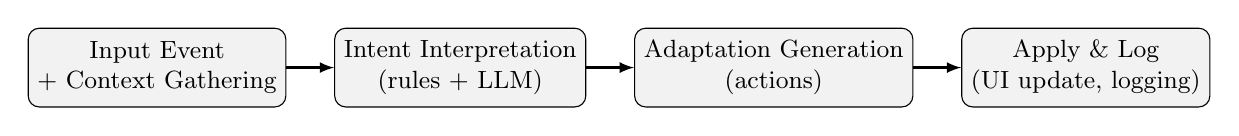
\begin{tikzpicture}[
    node distance=0.05\textwidth,
    font=\small,
    >=latex,
    every node/.style={draw, rounded corners, fill=gray!10, minimum width=0.18\textwidth, minimum height=1cm, align=center}
]
    % Nodes
    \node (input) {Input Event \\ + Context Gathering};
    \node[right=of input] (reason) {Intent Interpretation\\(rules + LLM)};
    \node[right=of reason] (adapt) {Adaptation Generation\\(actions)};
    \node[right=of adapt] (apply) {Apply \& Log\\(UI update, logging)};

    % Arrows
    \draw[->, thick] (input) -- (reason);
    \draw[->, thick] (reason) -- (adapt);
    \draw[->, thick] (adapt) -- (apply);
\end{tikzpicture}
\caption{Adaptation pipeline flow.}
\label{fig:adaptation-pipeline-flow}
\end{figure}

\subsection{Supported Adaptation Actions}
The framework supports a defined set of adaptation types that cover common accessibility needs. These include scaling or spacing adjustments for improved touch accuracy, font and contrast changes for better readability, and modality switches for hands-free interaction. The action set is deliberately kept broad enough to handle varied contexts, yet constrained enough to ensure reliable rendering across platforms (more details in Chapter~\ref{ch:chapter5}).

\subsection{Continuous Learning and Feedback Loop}
A central design principle is that adaptations are not static changes. The system maintains a history of recent interactions for each user, enabling it to identify recurring patterns such as frequent miss-taps or repeated modality switches. When such patterns are detected, the backend can suggest persistent adjustments; for example, permanently enlarging a frequently used UI element, reducing the need for smaller repeated actions.

\subsection{Design Considerations}
\begin{itemize}
    \item \textbf{Accessibility Focus:} All supported actions are chosen to address motor, visual, and input-related impairments, ensuring that adaptations enhance rather than complicate interaction.
    \item \textbf{Real-Time Performance:} Low-latency communication ensures that adaptations are applied quickly enough to feel seamless.
    \item \textbf{Reliability:} Rule-based logic ensures that adaptations continue to function even if LLM-based reasoning is temporarily unavailable.
    \item \textbf{Extensibility:} The action set and event format are flexible enough to incorporate new adaptation types and modalities in future deployments.
\end{itemize}
By combining immediate, context-aware changes with a persistent feedback loop, the dynamic adaptation mechanisms give the framework its ability to evolve alongside the user’s needs, making it more effective over time.

\section{Chapter Summary}
This chapter has presented the system design and architecture of the multimodal AI-driven framework for dynamic UI adaptation, focusing on its ability to deliver personalised, accessibility-oriented solutions for motor-impaired, visually impaired, and hands-free users. The framework is built around a modular three-layer architecture: the Frontend Layer, Input Adapter Layer, and SIF Backend Layer that enables the seamless integration of multiple input modalities, including touch, voice, and gestures, and the delivery of real-time UI adaptations.

The architectural design emphasises modularity, scalability, generalisability, and accessibility, creating a solid foundation for extension into other domains such as healthcare and gaming. Communication between layers is handled through WebSocket for low-latency updates and HTTP for reliable profile and debugging operations, while MongoDB and a standardised JSON contract ensure scalability and flexibility in storing and processing interaction data.
Together, these elements provide a framework capable of addressing real-world accessibility needs today.

%Chapter 4
\chapter{Smart Intent Fusion (SIF)}
\label{ch:chapter4}
\section{Introduction to Smart Intent Fusion}
Smart Intent Fusion (SIF) is the central intelligence layer of the proposed multimodal AI-driven UI adaptation framework, responsible for transforming raw, heterogeneous user input signals into concrete, context-aware interface adaptations. 
Where the Frontend Layer renders the UI and the Input Adapter Layer standardises events, SIF performs the reasoning step. Architecturally, SIF occupies the central position in the adaptation loop, receiving standardised events from the Input Adapter Layer, combining them with user profile and context data, and returning validated adaptations back to the frontend for immediate application. This placement ensures that every adaptation decision is both context-aware and modality-agnostic, allowing the framework to maintain consistent behaviour regardless of how the interaction was initiated.
it fuses current interaction data with user profiles, accessibility requirements, and recent interaction history to infer the user’s underlying intent and translate this into actionable UI changes.

The motivation for SIF stems from a simple but critical challenge in accessibility-focused HCI:
users rarely interact with a system through a single, perfectly clean input channel. Instead, interactions are often multimodal, noisy, and incomplete. A motor-impaired user may miss-tap a button but also issue a supporting voice command. A visually impaired user may attempt to activate a control by gesture but with low confidence, relying on high-contrast cues to complete the action. Traditional rule-based adaptive systems tend to process these signals independently, missing the opportunity to combine them into a unified, more reliable understanding of the user’s goal.

SIF addresses this gap through a hybrid reasoning approach:
\begin{itemize}
    \item Rule-based logic handles deterministic adaptations for example, “if miss\_tap on target → increase size by 1.5×” ensuring baseline accessibility support and fast response times even without AI availability.
    \item LLM-driven reasoning can process richer multimodal context and can propose creative or proactive adaptations that go beyond fixed rules such as switching to voice mode after repeated input struggles, or combining voice + gesture input to trigger a button instantly.
    \item Multi-Agent SIF (MA-SIF) extends this further by distributing reasoning across specialised LLM agents (UI, Geometry, Input or more) and validating results through a dedicated Validator Agent to reduce hallucinations and conflicting actions as well ensuring the necessary validation.
\end{itemize}

The SIF layer sits behind well-defined APIs:
\begin{itemize}
    \item WebSocket endpoint \texttt{/ws/adapt} for low-latency, real-time adaptation suggestions.
    \item HTTP endpoints like \texttt{/profile} for profile management, or \texttt{/full\_history} for developer tooling and debugging.
\end{itemize}
These endpoints use a strict JSON contract, making it easy for any frontend platform to connect and work with the backend. This ensures that the system remains flexible and can handle different input modalities.

A defining feature of SIF is its integration with persistent user profiles stored in MongoDB. These profiles encapsulate three layers of information: static attributes such as preferred font size or contrast mode, learned preferences derived from recurring interaction patterns, and contextual data including recent history and environmental details. By merging these dimensions with each incoming event, SIF can make decisions that are not only responsive to the user’s current action but also aligned with their long-term accessibility needs.
By fusing this profile data with incoming events, SIF maintains a continuous personalisation loop progressively adapting the UI to match the user’s abilities and context over time.

For example:
\begin{itemize}
    \item A profile with \texttt{motor\_impaired: true} will bias adaptations towards larger controls and simplified layouts.
    \item Repeated history of slider misses may lead to permanent slider thumb enlargement.
    \item A hands-free preference can automatically promote voice/gesture-driven navigation in relevant contexts.
\end{itemize}

In the context of this thesis, SIF is not only an internal backend feature, it is the core research contribution.
The remainder of this chapter expands on the theoretical underpinnings of SIF, its integration with user profiles and multimodal fusion, the prompt engineering strategies for guiding LLM behaviour, the architecture of its multi-agent extension, and the performance metrics used to evaluate its effectiveness.
% Event Flow Diagram: Abstract SIF Reasoning Pipeline (Vertical Layout)
\begin{figure}[h]
\centering
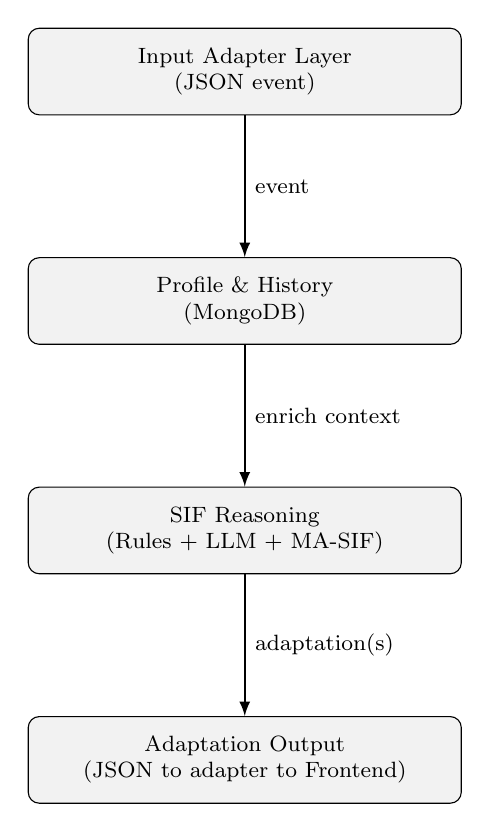
\begin{tikzpicture}[
    node distance=1.8cm,
    font=\small,
    >=latex,
        every node/.style={font=\footnotesize},
    sbox/.style={draw, rounded corners, fill=gray!10, minimum width=5.5cm, minimum height=1.1cm, align=center}
]
    % Nodes (vertical stack)
        \node [sbox] (adapter) {Input Adapter Layer \\ \footnotesize (JSON event)};
        \node [sbox, below=of adapter] (profile) {Profile \& History \\ \footnotesize (MongoDB)};
        \node [sbox, below=of profile] (reason) {SIF Reasoning \\ \footnotesize (Rules + LLM + MA-SIF)};
        \node [sbox, below=of reason] (output) {Adaptation Output \\ \footnotesize (JSON to adapter to Frontend)};

        % Arrows
        \draw[->, thick] (adapter) -- (profile) node[midway,right]{event};
        \draw[->, thick] (profile) -- (reason) node[midway,right]{enrich context};
        \draw[->, thick] (reason) -- (output) node[midway,right]{adaptation(s)};
\end{tikzpicture}
\caption{Abstract event flow in Smart Intent Fusion: events from the Input Adapter are enriched with profile/context, processed by rule-based and LLM/MA-SIF reasoning, and returned as adaptation outputs to the frontend.}
\label{fig:sif-event-flow}
\end{figure}

\section{Theoretical Foundations of Smart Intent Fusion}
The idea behind Smart Intent Fusion is simple:
\\ users don’t interact with a UI in one clean and perfect way. In real life, inputs are messy, mixed, and often incomplete. A person might tap the wrong spot on a button, then say a voice command to make sure it worked. Someone using gestures might point at something but not be perfectly accurate, so they rely on extra visual cues to finish the task. A lot of current adaptive systems still process these signals separately, and that means they miss the chance to combine them into a clearer picture of what the user actually wanted.

Smart Intent Fusion tries to fix that by taking all the inputs together: touch, keyboard, voice, gestures and mixing them with what the system already knows about the user (their profile, their history of interactions, and their accessibility needs). This way, it can guess the real intent and adapt the UI in the most helpful way.

\subsection{Multimodal Fusion}
In HCI, “multimodal fusion” just means combining different types of input to get a more reliable or richer understanding of the user’s action. 
\\This can be done in a few ways:
\begin{itemize}
    \item \textbf{Early fusion}: merge the raw signals before interpreting them (e.g., combining the coordinates of a tap with the audio of a voice command immediately). \\
    → Useful when two inputs happen at the exact same moment.
    \item \textbf{Late fusion}: process each input type separately first, then merge the interpreted results (e.g., “voice command = unlock” + “miss-tap near unlock button” → final decision = trigger Unlock button).\\
    → This is where most SIF reasoning happens.
    \item \textbf{Hybrid fusion}: a mix of both, sharing some data early but also combining results later. \\
    → Used when one modality’s data can make another modality’s interpretation more accurate.
\end{itemize}
SIF uses the hybrid approach. The Input Adapter Layer already standardises each input into a clean JSON format, but the fusion step happens in the backend where the current event, past history, and profile are all processed and fused together. This makes it possible to combine patterns like “miss-tap + voice command” into one clear adaptation. In the overall architecture described in Chapter~\ref{ch:chapter3}, this fusion step is the bridge between raw input handling and adaptation generation. By sitting in the backend, SIF can remain entirely modality-agnostic while still benefiting from the structured event format defined by the Input Adapter Layer. This ensures that even when new input methods are introduced in the future, the fusion logic can remain unchanged, relying on the same JSON schema and profile-context pipeline.

\subsection{Intent Inference}
The main goal of SIF is not just to log inputs, but to figure out \textit{why} the user did them. This is called intent inference. In other words, we want the system to answer the question: “What was the user trying to do?”
If the system knows the intent, it can choose the best adaptation. The inference process is always profile-aware. Each decision is informed by a combination of static preferences (such as font size or contrast mode), learned patterns from past usage (such as repeated difficulty with sliders), and short-term contextual data (such as the most recent interactions). This means that two users producing the same input sequence could receive different adaptations if their profiles and histories differ, keeping the interaction completely personalised. 
\\For example:
\begin{itemize}
    \item If the intent is to press “Unlock” but the user misses, the adaptation could be to enlarge the button and trigger it right away.
    \item If the intent is to adjust a thermostat but the user struggles with the slider, the adaptation could be to switch to voice control and increase the slider size.
\end{itemize}

This is where LLMs can help. They are good at reasoning about context, combining clues, and filling in gaps when inputs are unclear. The downside is that they can be slow, be costly to run, and sometimes “hallucinate” an answer that doesn’t make sense even if its not defined in the prompt. That’s why SIF uses a \textbf{hybrid} approach:
\begin{itemize}
    \item \textbf{Rules} handle clear, simple cases with instant feedback.
    \item \textbf{LLM reasoning} handles more complex or ambiguous cases.
\end{itemize}

\subsection{Why Hybrid Works Best}
A purely rule-based system is predictable but rigid. It can only respond to situations that were thought of in advance. A purely LLM-based system is flexible but not always reliable, especially when it needs to work in (close to) real time for accessibility.
By combining both:
\begin{itemize}
    \item The rules guarantee that basic accessibility changes (like increasing size after a miss-tap) always work. For example:
    \begin{verbatim}
        IF event_type == "miss_tap" AND profile.motor_impaired == true
        THEN action = increase_button_size(target, 1.5)
    \end{verbatim}
    \item The LLM adds creativity and can adapt to situations the rules didn’t cover, like combining unusual input patterns, proposing a mode switch for hands-free use or even something entirely new.
\end{itemize}

\subsection{Connection to Accessibility}
The whole point of this is to improve accessibility for different kinds of users:
\begin{itemize}
    \item \textbf{Motor-impaired:} combine multiple input signals to avoid repeated failed attempts.
    \item \textbf{Visually impaired:} recognise when visual feedback is not enough and trigger higher-contrast or bigger fonts automatically.
    \item \textbf{Hands-free:} allow combinations like voice + gesture to instantly activate actions.
\end{itemize}

In short, the theoretical base for SIF comes from multimodal fusion, intent inference, and hybrid reasoning. These ideas are not new in HCI, but this framework applies them with a strong focus on accessibility and personalisation, and makes them work in real time with cross-platform UI code. For example, a motor-impaired user who misses a lock button twice and then issues a voice command might trigger a combined adaptation: the UI immediately enlarges the button for future taps, but also switches the interface to voice-first mode for the current session. This ability to layer short-term fixes on top of long-term adjustments is what makes SIF more than just a reactive system, it is a continuously learning adaptation layer.

\section{User Profile and Context Integration}
For Smart Intent Fusion to be truly “smart,” it needs more than just the current event it is processing. If SIF reacted to every tap, voice command, or gesture without knowing who the user is or how they usually interact, it would behave like a generic accessibility script rather than a personalised adaptation system. That’s why the user profile and interaction context form the backbone of the reasoning process. They give SIF a sort of memory/personality, and the ability to adapt over time, not just in the moment.
When a new event comes in like a tap, miss-tap, voice command, or gesture, SIF doesn’t look at it in isolation. It combines that event with:
\begin{enumerate}
    \item \textbf{The user profile} – a stored record in MongoDB with accessibility flags, preferred modalities, and UI settings.
    \item \textbf{Interaction history} – the last 10 events that show patterns or repeated problems.
    \item \textbf{Current UI context} – optional metadata about what’s on screen, where buttons are placed, and their sizes.
\end{enumerate}
This means SIF can make decisions that are personal and context-aware, not just reactive.

\subsection{User Profiles}
A user profile stores the information that makes one person’s interaction style different from another’s.
This can include accessibility needs (motor-impaired, visually impaired, hands-free preferred), preferred input modalities, and baseline UI settings like font size, contrast mode, and button scale. It can be seen as the \textbf{memory} of the system.
When combined with a short history of recent interactions, this profile turns SIF from a static decision engine into a continuous learning system. 

Without profiles, SIF could still make adaptations, however they would always be reactive and temporary.
For example:
\begin{itemize}
    \item If a user with tremors keeps missing a button, the button might get enlarged for that session, but as soon as they restart the app, it would shrink back.
    \item If a user prefers voice input, SIF wouldn’t know to automatically switch to voice mode when they struggle with touch, instead it would have to come up on its own that this switch is needed for this user.
\end{itemize}
Profiles ensure these adaptations stick and get better over time.

\subsection{User Profile Structure}
In the backend, each profile is a JSON document in the \texttt{profiles} collection of a MongoDB database. It’s indexed by \texttt{user\_id} so the system can look it up instantly whenever a new event arrives. A typical structure looks like this:

\begin{lstlisting}[language=json, caption=Simplified User Profile Example]
{
  "user_id": "user_123",
  "accessibility_needs": { "motor_impaired": true },
  "input_preferences": { "preferred_modality": "voice" },
  "ui_preferences": { "font_size": 16 },
  "interaction_history": [
     { "action":"increase_button_size", "target": "all", "value": 1.2 },
     { "action":"increase_font_size", "target": "all",  "value": 1.1 } 
  ]
}
\end{lstlisting}

This design keeps it simple but flexible. Architecturally, each profile contains:
\begin{itemize}
    \item \texttt{accessibility\_needs}: flags that tell SIF what kind of adaptations to prioritise.
    \item \texttt{input\_preferences}: helps the system decide which modality to switch to when needed.
    \item \texttt{ui\_preferences}: baseline visual parameters such as font size and contrast mode.
    \item \texttt{interaction\_history}: capped log of recent events to support continuous learning.
\end{itemize}
MongoDB’s indexing means the profile can be retrieved in milliseconds, even with a large user base, and capped histories ensure lookups are fast.

\subsection{How Profiles Affect Decisions}
When an event comes in, the backend follows a clear process:
\begin{enumerate}
    \item Load the profile from MongoDB using the \texttt{user\_id}. If it doesn’t exist yet, create a new default profile.
    \item Combine the event with the last few interactions from the history.
    \item Pass the profile, history, and current event into the Smart Intent Fusion reasoning step.
\end{enumerate}
This context completely changes how SIF decides on adaptations.\\\\
Some examples of influenced decisions:

\textbf{Example 1: Motor-impaired user with repeated miss-taps}\\
If the last three events in history are miss-taps on the same “Unlock/Lock” button, and \texttt{motor\_impaired} is true in their profile, SIF might do two things at once:
\newpage
\begin{lstlisting}[language=json, caption={Possible motor-impaired user adaptations}]
[
  {"action": "increase_button_size", "target": "button_unlock", "value": 1.5, "reason": "Multiple miss-taps detected, enlarging button for better accessibility"},
  {"action": "highlight_border", "target": "button_unlock", "reason": "Increase button visibility for the user"}
]
\end{lstlisting}
Without the profile, it might have just enlarged the button once and moved on.

\textbf{Example 2: Hands-free preferred user}
A user with \texttt{"hands\_free\_preferred": true} points at a device card (gesture) and says “turn on the lights.”
SIF reasoning can fuse these into:
\begin{lstlisting}[language=json, caption={Hands-free user intent fusion}]
{
  "action": "trigger_button",
  "target": "button_light",
  "reason": "Gesture pointing + voice 'Turn on the lights' detected for hands-free user",
  "intent": "Activate Lights"
}
\end{lstlisting}
Because of the profile, SIF is confident enough to trigger the button immediately without asking for physical confirmation.

\subsection{Continuous Learning from History}
Profiles are not static. Every interaction is logged in the \texttt{interaction\_history} and can influence future decisions. The interaction context can be seen as the system's \textbf{short-term awareness}.
This makes SIF a learning system:
\begin{itemize}
    \item If a user keeps manually enabling high-contrast mode, the system can update \texttt{contrast\_mode} in their profile so it’s always on by default.
    \item If increasing a button size significantly reduces miss-taps, that size can become the new permanent baseline in \texttt{ui\_preferences}.
    \item If switching to voice mode solves repeated touch struggles, the profile can be updated to favour voice by default.
\end{itemize}
This feedback loop means the user doesn’t need to “train” the system manually, it adapts naturally as they use it. If SIF only looked at the current event, it would miss important patterns and make short-sighted decisions.
With profile + history + event combined:
\begin{itemize}
    \item Adaptations can be proactive instead of reactive.
    \item The UI can stay consistent between sessions.
    \item The system can learn what really helps the user over time.
\end{itemize}
From an accessibility perspective, this is the difference between a generic interface that occasionally helps and a personalised tool that feels like it understands the user.

\subsection{Role in Accessibility}
User profiles are the backbone of accessibility-focused adaptations in this framework. They act as a persistent memory of the user’s abilities, preferences, and interaction challenges, enabling the system to make targeted, proactive adjustments rather than relying solely on short-term reactive changes. By storing explicit accessibility flags alongside learned behavioural patterns, profiles allow SIF to tailor the interface to an individual user in ways that are both short-term and long-term.

From an accessibility perspective, profiles influence SIF’s reasoning in three key user categories:
\begin{itemize}
    \item \textbf{Motor-Impaired Users:} Profile flags such as \verb|motor_impaired: true| prioritise adaptations that reduce fine motor precision requirements. This can include:
    \begin{itemize}
        \item Enlarging touch targets (buttons, sliders) and increasing spacing to prevent accidental taps.
        \item Offering alternative modalities such as voice commands or keyboard navigation to bypass touch interaction altogether.
        \item Retaining enlarged target sizes across sessions once repeated miss-taps are detected.
    \end{itemize}

    \item \textbf{Visually Impaired Users:} When \verb|visual_impaired: true| is set, adaptations aim to maximise visual clarity. Examples include:
    \begin{itemize}
        \item Switching to high-contrast themes and bold colour schemes to align with WCAG 2.1 contrast requirements.
        \item Increasing font sizes and icon scales to meet text accessibility guidelines.
        \item Highlighting the active element with a strong focus border or magnified overlay to improve navigation feedback.
    \end{itemize}

    \item \textbf{Hands-Free Users:} Profiles with \verb|hands_free_preferred: true| bias SIF towards non-touch input modes, reducing physical interaction demands. Adaptations may involve:
    \begin{itemize}
        \item Automatically switching to voice or gesture navigation when interaction struggles are detected.
        \item Providing clear, speech-friendly UI labels and tooltips to improve command recognition accuracy.
        \item Simplifying layouts by reducing the number of visible controls at once, making it easier to select elements through voice or gesture.
    \end{itemize}
\end{itemize}

By embedding these accessibility considerations directly into the profile structure, SIF can reason in a way that is both context-aware and user-specific. This allows the system to:
\begin{enumerate}
    \item Anticipate needs before errors occur (e.g., pre-emptively enlarging critical controls for a motor-impaired user on a small screen).
    \item Ensure adaptations persist across sessions, avoiding the frustration of having to reconfigure accessibility settings each time.
    \item Combine profile knowledge with real-time interaction patterns, enabling nuanced decisions such as \emph{“keep high contrast on by default, but also enable voice mode when the user is multitasking”}.
\end{enumerate}

\section{Modeling Multimodal Input Fusion}
Smart Intent Fusion doesn’t just take one input, it collects \textbf{multiple inputs from different modalities} like touch, voice, gestures, and more. Then fuses them into a single, well-reasoned adaptation. This process is called \textit{multimodal input fusion}.
Without fusion, the system would treat each event separately. A miss-tap would trigger one adaptation, and a voice command would trigger another, without realising both were aimed at the same action. With fusion, those two inputs can be combined into one confident and more helpful response which saves time and reduces frustrations. Furthermore, the user profile and interaction history also directly affect how this fusion works. A hands-free preferred user will have a lower threshold for fusing gesture + voice, but a visually impaired user’s profile might cause SIF to always add a “highlight” adaptation when triggering elements via voice, even if not strictly necessary. If history shows repeated failures for a certain modality, its weight in fusion decisions can be reduced. For users with impairments, every extra action is extra effort. Because of how the fusion is designed, it cuts down on unnecessary steps so the UI adapts faster and smarter to the user’s needs.

\subsection{Event Standardisation}
Before any fusion can happen, the raw input needs to be standardised.
Every frontend in the framework Flutter, SwiftUI or a future VR client converts its local input data into the same JSON contract. This is handled by the Input Adapter Layer as described earlier.

A standardised event looks like this:
\begin{lstlisting}[language=json, caption={Standardised Event Example}]
{
  "event_type": "miss_tap",
  "source": "touch",
  "timestamp": "2025-08-04T14:41:00Z",
  "user_id": "user_123",
  "target_element": "button_unlock",
  "coordinates": {"x": 210, "y": 640},
  "confidence": 0.8,
  "metadata": {"UI_element": "button"}
}
\end{lstlisting}
This contract ensures:
\begin{itemize}
    \item \textbf{Cross-platform compatibility}: all clients speak the same “language” to the backend.
    \item \textbf{Dynamic field names}: fields like \texttt{event\_type} and \texttt{target\_element} can be extended and modified without breaking existing logic.
    \item \textbf{Extensibility}: new modalities can be added (like gaze tracking) without breaking existing clients.
\end{itemize}
By the time the event reaches SIF, it doesn’t matter whether it came from a phone, desktop, or VR headset, it always adheres to the same format for the backend.
As said earlier SIF uses a hybrid approach for multimodal input fusion. The Input Adapter handles basic pre-processing (similar to early fusion), but the actual reasoning, deciding what adaptations to apply happens in the backend using late fusion.

\textbf{Example: Touch + voice} \\
Let’s say a motor-impaired user taps just to the right of the “Lock/Unlock” button and, within a second, says “Unlock.”
Individually, the miss-tap could trigger an enlargement of the button and the voice command could trigger the unlocking action. However, with multimodal fusion, the system can understand that both inputs are related and prioritize the unlocking action while also enlarging the button for better accessibility.

With SIF fusion, the system sees both in context:

\begin{lstlisting}[{language=json}, caption=Example of Multimodal Fusion]
[
  {"action": "increase_button_size", "target": "button_unlock", "value": 1.5, "reason": "Miss-tap detected near Unlock button"},
  {"action": "trigger_button", "target": "button_unlock", "reason": "Voice command 'unlock' detected in combination with miss-tap"}
]
\end{lstlisting}
Now the button is both enlarged for future use and triggered immediately, reducing the number of actions the user needs to take, simplifying the interaction which is useful for motor-impaired users.

\subsection{Timing and Confidence}
SIF's LLM reasoning can also consider \textbf{when} and \textbf{how confidently} an input happened based on two fields from the standardised event:
\begin{itemize}
    \item \textbf{Timing}: events close together in time (e.g., within 1–2 seconds) are more likely to be related.
    \item \textbf{Confidence}: each modality can provide a confidence score (e.g., gesture detection might be 0.7 certainty). Lower confidence might require a second modality before acting.
\end{itemize}
For example, a low-confidence gesture to point at a button might do nothing alone, but if followed by a high-confidence voice command naming that button, SIF can treat them as a combined intent.

\subsection{LLM Reasoning in Fusion Decisions}
While the fusion process benefits from deterministic rules for speed and reliability, one of the key innovations of SIF is its ability to leverage LLM reasoning to interpret and combine multimodal inputs in a context-aware way. 

Once standardised events reach the backend, they are not processed in isolation. Each event is enriched with:
\begin{itemize}
    \item \textbf{User profile data:} accessibility flags, preferred modalities, and baseline UI settings.
    \item \textbf{Interaction history:} the most recent events, revealing repeated struggles or patterns.
    \item \textbf{Contextual metadata:} details about the UI state (e.g., which elements are visible), UI element type, environment and more.
\end{itemize}

This enriched dataset is then included in the LLM prompt, allowing the model to reason comprehensively about the user’s intent across modalities.  
For example, instead of treating:
\begin{itemize}
    \item a low-confidence “point” gesture at a thermostat slider, and
    \item a voice command “set temperature to 22”
\end{itemize}
as separate actions, the LLM can infer that they describe the same goal and produce a single adaptation: 
\begin{lstlisting}[language=json]
{
  "action": "adjust_slider",
  "target": "slider_thermostat",
  "value": 22,
  "reason": "Gesture and voice command combined to adjust temperature"
}
\end{lstlisting}

By bringing together different types of input modalities, user’s preferences, and their recent actions, SIF can suggest changes that are not only accurate but also anticipate what will help the user most. This means the system can adapt quickly and make the interface easier to use based on what the user's most probable intent was.

\section{Rule-Based Logic and LLM-Driven Adaptation}
Smart Intent Fusion uses two very different ways to decide what adaptation to apply:
\begin{itemize}
    \item \textbf{Rule-based logic} handles clear, deterministic cases where the system can apply a known adaptation based on the event type and user profile. It is instant, and predictable.
    \item \textbf{LLM-driven reasoning} uses the Gemini API to process complex, multimodal contexts and propose creative adaptations that go beyond simple rules.
\end{itemize}
Both have strengths and weaknesses, which is why the framework combines them instead of choosing one.

\subsection{Rule-Based Logic}
Rule-based logic works by matching incoming events to predefined conditions and applying a fixed response.\\
For example:
\begin{lstlisting}[language=python, breaklines]
    if event.event_type == "miss_tap":
        return {"action": "increase_button_size", "target": event.target_element, "value": 1.5}
\end{lstlisting}
Advantages:
\begin{itemize}
    \item \textbf{Simplicity}: Easy to implement and understand.
    \item \textbf{Speed}: Instantaneous responses to known events.
    \item \textbf{Predictability}: Consistent behavior for similar inputs and no risk of unintended consequences like hallucinations.
    \item \textbf{Baseline guarantee}: Acts as a safety net so that critical accessibility features still work if the LLM is unavailable, slow to respond, or returns unusable output.
\end{itemize}
Limitations:
\begin{itemize}
    \item Can only handle cases explicitly programmed in advance.
    \item No ability to combine signals in creative ways.
    \item Doesn’t learn new patterns unless a developer updates the rules.
\end{itemize}
This means that while rule-based logic is fast and reliable, it can also be rigid and unable to adapt to new situations without human intervention. In SIF, they are deliberately kept lightweight, mostly as a mock or backup layer for LLM-driven reasoning.


\subsection{LLM-Driven Reasoning}
The LLM can reason about the event, user profile, and history together to try and infer the user's intent more deeply. It can make connections that rules would miss, such as:
\begin{itemize}
    \item Combining a miss-tap with a voice command into a single action.
    \item Switching to a different modality when it detects repeated failure in the current one.
    \item Proposing multiple coordinated adaptations for one intent.
\end{itemize}
Advantages:
\begin{itemize}
    \item \textbf{Flexibility}: Can adapt to new situations without explicit programming by the developer.
    \item \textbf{Context-aware}: Takes profile and history into account naturally.
    \item \textbf{Learning}: Can improve over time by learning from user interactions and feedback.
\end{itemize}
Limitations:
\begin{itemize}
    \item \textbf{Less predictable}: May generate unexpected or irrelevant responses.
    \item \textbf{Slower}: Network call + reasoning time.
    \item \textbf{Needs validation}: Output must be checked more thoroughly before applying.
\end{itemize}

\subsection{Hybrid Approach in SIF}
In practice, SIF doesn’t fully choose between the two, it blends them:
\begin{enumerate}
    \item \textbf{Rules first}: If the event matches a clear, high-confidence rule, apply it immediately, this is mostly done in the frontend by the user profile.
    \item \textbf{LLM second}: Use the model for complex or ambiguous cases, or to suggest extra adaptations beyond the rules.
    \item \textbf{Timeout Fallback}: If the LLM times out or fails, return rule-based or other LLM output only.
\end{enumerate}
This ensures that basic accessibility features always work, while still allowing for creative, context-aware adaptations when needed. In other words, the rules form the “floor” of the system (the minimum guaranteed level of accessibility) while the LLM can raise the ceiling by adapting to more complex, ambiguous, or novel situations. Users are never left waiting for AI responses that might never come, and the system remains responsive even in worst-case scenarios.

\subsection{Heatmap Analysis}

To further refine adaptation decisions, the backend can analyze interaction heatmaps derived from user event logs. By aggregating tap coordinates and gesture paths, the system identifies problematic UI regions (e.g., frequently missed buttons) and adapts layouts or element sizes accordingly. This data-driven approach supports continuous improvement and personalization, especially for users with evolving accessibility needs. By using tap frequency, the backend can suggest adaptations like repositioning elements or enlarging hit areas, enhancing usability.

\section{Multi-Agent Smart Intent Fusion (MA-SIF)}
While a single LLM can process events and suggest adaptations, it often tries to “do everything” at once.
That makes it harder to constrain, more prone to hallucinations, less predictable and in some cases slower (depending on workload).
Multi-Agent Smart Intent Fusion (MA-SIF) solves this by splitting the reasoning into specialised agents, each focused on one domain of UI adaptation, and then combining their outputs through a Validator Agent.
This design brings the benefits of modularity, parallelism, and role-specific constraints, all of which improve reliability and make the system easier to maintain.

\subsection{Why Multiple Agents?}
When one model is asked to handle UI changes, geometry adjustments, input mode switching, and validation all at once, several problems appear:
\begin{itemize}
    \item The prompt becomes long and vague.
    \item Allowed actions become harder to enforce and turn into hallucinations.
    \item Reasoning gets scattered between unrelated concerns.
\end{itemize}
By giving each agent a clear role, their prompts can be short, specific, and easy to maintain.
For example, the UI agent only ever sees actions like \texttt{increase\_font\_size} or \texttt{increase\_contrast}, while the Geometry agent only deals with spatial changes like \texttt{increase\_button\_size} or \texttt{adjust\_spacing}.
This separation means that each agent can focus on its specific task without being distracted by unrelated concerns. Parameters can be tuned independently for each agent, allowing for more precise control over their behavior (e.g., lower temperature for Geometry, slightly higher for Input). Finally, debugging becomes easier as each agent's logic is contained and easier to follow.

\subsection{Agent Roles}
At a high level, MA-SIF in this thesis's current configuration, consists of four specialised LLM agents: 
\begin{enumerate}
    \item a \textbf{UI Agent} for visual and interactive adaptations, 
    \item a \textbf{Geometry Agent} for spatial changes and layout simplification, 
    \item an \textbf{Input Agent} for modality switching and interaction simplification, 
    \item a \textbf{Validator Agent} for conflict resolution and accessibility compliance. 
\end{enumerate}
Each has a narrow focus, defined prompts, and a limited set of allowed actions, making their reasoning predictable and easier to validate. They have clearly defined scopes of responsibility, and their roles are deliberately narrow to keep prompts concise, outputs predictable, and debugging straightforward. \textbf{The UI Suggestion Agent} is concerned purely with visual accessibility changes such as increasing font size, toggling high-contrast mode, or displaying contextual tooltips. For example, when a visually impaired user interacts with a dense text block, this agent might output an adaptation like increasing the global font scale by 1.2×.

The \textbf{Geometry Suggestion Agent} deals with spatial layout changes and the physical dimensions of interactive elements. It might recommend increasing the size of a button, expanding the hit area of a slider, or adding extra spacing between cards in a list. For example, a motor-impaired user who repeatedly misses a button may trigger an output to enlarge that specific button by 1.5× while keeping the rest of the interface unchanged.

The \textbf{Input Suggestion Agent} focuses on modality switching and simplifying interaction pathways. It is capable of suggesting transitions between touch, keyboard, voice, or gesture modes, as well as proposing layout simplifications to reduce cognitive load. For instance, if a user struggles with touch but succeeds with voice commands, this agent can suggest switching to voice-first navigation, potentially combined with a reduced interface complexity.

Finally, the \textbf{Validator Agent} operates after all others have completed their reasoning. This is the most computationally demanding role, as it must examine every proposed adaptation in detail, identify and remove duplicates, verify that all actions are allowed, and ensure that no output falls outside safe parameter ranges. It also resolves potential conflicts, such as two agents targeting the same element with incompatible values. Because of the breadth of this responsibility, the validator uses a larger Gemini model, a higher timeout of 30 seconds, and a dynamic thinking budget.

\subsection{Adaptation Flow}
When an event arrives at the backend, the fusion process begins by loading the user’s profile and recent interaction history from MongoDB. This contextual data is then sent to each non-validator agent, alongside the event itself. The prompt for each agent is tailored to its domain, ensuring that the LLM only receives relevant instructions and the list of actions it is permitted to output.

Once each agent has processed the event, their suggestions are collected. Importantly, the system is tolerant of partial failures, if one or more agents fail to return a result due to a timeout or API error, the remaining agents’ outputs are still retained. These partial results are then passed to the Validator Agent, which merges them into a coherent and conflict-free final adaptation set. Another possibility is fusing LLM adaptations with rule-based suggestions to create a hybrid output when one or more agents fail.

If the validator itself fails, either due to malformed output or a processing error, the system does not discard all results. Instead, it falls back to returning the raw, unvalidated suggestions from the agents since the output may still be more useful than rule-based alternatives. Only if all agents fail to produce output does the framework revert to the rule-based \texttt{mock\_fusion} fallback. This layered approach ensures that useful adaptations are preserved whenever possible, rather than being lost due to a single point of failure.

\begin{figure}[ht]
\centering
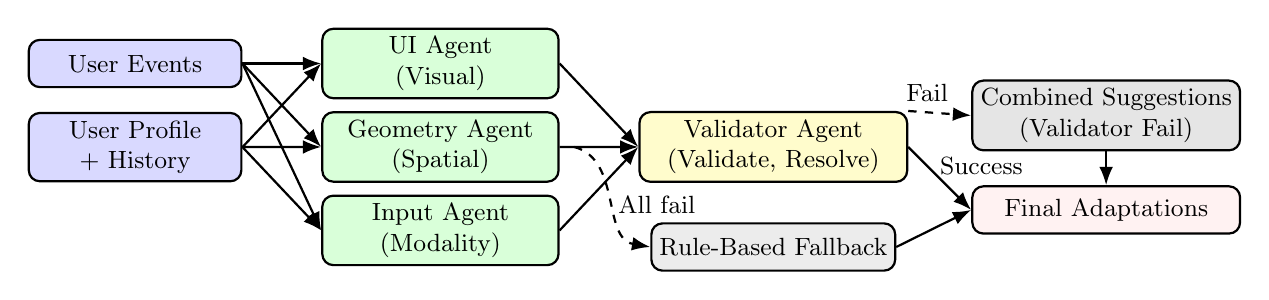
\begin{tikzpicture}[
    scale=0.93,
    font=\small,
    >=Latex,
    node distance=6mm and 10mm,
    block/.style={draw, rounded corners=4pt, thick, align=center, minimum height=6mm, minimum width=27mm, inner sep=1mm},
    input/.style={block, fill=blue!15},
    agent/.style={block, fill=green!15, minimum width=30mm},
    validator/.style={block, fill=yellow!20, minimum width=34mm},
    fallback/.style={block, fill=gray!15, minimum width=30mm},
    suggest/.style={block, fill=gray!20, minimum width=34mm},
    final/.style={block, fill=pink!20, minimum width=34mm},
    line/.style={->, thick},
    dline/.style={->, thick, dashed}
]

% Inputs (left column)
\node[input] (events) {User Events};
\node[input, below=3mm of events] (profile) {User Profile\\+ History};

% Agents (middle column)
\node[agent, right=10mm of events] (ui) {UI Agent\\(Visual)};
\node[agent, below=1.5mm of ui] (geo) {Geometry Agent\\(Spatial)};
\node[agent, below=1.5mm of geo] (inp) {Input Agent\\(Modality)};

% Validator + fallback (right column)
\node[validator, right=10mm of geo] (val) {Validator Agent\\(Validate, Resolve)};
\node[fallback, below=5mm of val] (fb) {Rule-Based Fallback};

% Results (far right)
\node[suggest, right=8mm of val, yshift=4mm] (comb) {Combined Suggestions\\(Validator Fail)};
\node[final, right=8mm of val, yshift=-8mm] (final) {Final Adaptations};

% Inputs to agents (direct arrows)
\draw[line] (events.east) -- (ui.west);
\draw[line] (events.east) -- (geo.west);
\draw[line] (events.east) -- (inp.west);

\draw[line] (profile.east) -- (ui.west);
\draw[line] (profile.east) -- (geo.west);
\draw[line] (profile.east) -- (inp.west);

% Agents to validator
\draw[line] (ui.east) -- (val.west);
\draw[line] (geo.east) -- (val.west);
\draw[line] (inp.east) -- (val.west);

% All agents fail -> fallback
\draw[dline] ([xshift=2mm]geo.east) to[out=-15,in=170] node[above,pos=0.7,xshift=4.5mm]{All fail} (fb.west);

% Validator success/fail
\draw[line] (val.east) -- node[above,pos=0.6, xshift=4.5mm]{Success} (final.west);
\draw[dline] (val.north east) --  node[above,pos=0.3]{Fail} (comb.west);

% Combined/fallback to final
\draw[line] (comb.south) -- (final.north);
\draw[line] (fb.east) -- (final.west);

\end{tikzpicture}
\caption{Multi-agent SIF adaptation flow: user events and profile/history are processed by specialised agents, validated, and merged into final adaptations. Fallbacks ensure robustness.}
\label{fig:ma-sif-flow}
\end{figure}

\subsection{Dynamic Configuration}
A key advantage of MA-SIF is that it is configured almost entirely through the \texttt{sif\_config.json}, making it very adaptable without requiring backend code changes. Each agent’s behaviour can be fine-tuned individually including its allowed actions, model type, temperature, thinking budget, and timeout, simply by editing the configuration file. This flexibility extends to the ability to add new agents or duplicate existing ones with different focuses.

For instance, it is entirely possible to run two Geometry agents in parallel: one optimised for mobile devices with smaller screens and one tuned for desktop layouts. Both would analyse the same event and profile data but apply different heuristics in their prompts. The Validator Agent would then merge their suggestions, resolving overlaps and conflicts automatically. This makes it possible to create specialised agents for emerging modalities, such as gaze tracking in VR, without altering any core fusion logic.

This externalised configuration is particularly valuable in accessibility research, where rapid iteration is needed. 
For example, during a live user study, the prompt for the UI Agent can be adjusted to emphasise high-contrast themes over font scaling without redeploying the backend. 
Similarly, experimental agents for new modalities such as gaze tracking or haptic feedback can be added in minutes, allowing researchers or developers to test new adaptation strategies with minimal downtime.

\begin{lstlisting}[language=json,firstnumber=1, caption={Basic example of a 2-agent (+ validator) configuration}]
{
  "ui_agent": {
    "model_settings": {
        "model": "gemini-2.5-flash-lite",
        "temperature": 0.2,
        "thinking_budget": 0
    },
    "focus": ["visual adaptations"],
    "allowed_actions": ["increase_size", "increase_contrast", "reposition_element"],
    "prompt": "Given the event data, suggest UI adaptations for accessibility. Consider user profile and interaction history."
  },
  "geometry_agent": {
    "model_settings": {
        "model": "gemini-2.5-flash-lite",
        "temperature": 0.2,
        "thinking_budget": 0
    },
    "focus": ["spatial adaptations"],
    "model": "gemini-2.5-flash-lite",
    "allowed_actions": ["resize_element", "adjust_spacing", "simplify_layout"],
    "prompt": "Analyze the UI layout and suggest spatial adaptations to improve usability for motor-impaired users."
  },
  "validator_agent": {
    "model_settings": {
        "model": "gemini-2.5-flash",
        "temperature": 0.3,
        "thinking_budget": -1,
        "timeout": 30
    },
    "allowed_actions": ["switch_to_voice", "interpret_gesture", "recover_from_error", "increase_size", "increase_contrast", "reposition_element","resize_element", "adjust_spacing", "simplify_layout"],
    "prompt": "Validate proposed adaptations for conflicts, duplicates and inconsistencies based on user context, events and interaction history."
  }
}
\end{lstlisting}
Each agent configuration above specifies its model, temperature, and thinking budget, which control the LLM's behavior and output style. The \texttt{focus} field describes the agent's adaptation domain, while \texttt{allowed\_actions} restricts the set of suggestions to ensure predictable outputs. The \texttt{prompt} guides the agent's reasoning, and is dynamically extended at runtime with the current event (see Chapter~\ref{ch:chapter5}), user profile, and interaction history. This enables agents to generate personalized adaptation suggestions based on live user context, rather than relying solely on static instructions.

\subsection{Temperature and Thinking Budget}

Two key parameters control the behaviour of each LLM agent in MA-SIF: \textbf{temperature} and \textbf{thinking budget}.

\textbf{Temperature} determines the randomness and creativity of the model’s output. Lower values (e.g., 0.2) make the agent more deterministic, producing consistent and predictable suggestions—ideal for accessibility-focused UI changes where reliability is critical. Higher values (e.g., 0.7 or 1.0) increase creativity and output diversity, but can introduce unpredictability or hallucinations, which may be undesirable for critical adaptations.

\textbf{Thinking budget} limits the number of reasoning steps or computational effort before the agent responds. A budget of 0 results in minimal reasoning and fast, direct answers. Higher budgets allow the agent to consider more factors, leading to more nuanced or complex suggestions. Negative values (e.g., -1) remove the limit, enabling extensive reasoning, useful for roles like the Validator Agent, which must resolve conflicts and ensure schema compliance.

\textbf{Effect on Reasoning:}
\begin{itemize}
    \item Lower temperature and budget: Fast, predictable, and simple adaptations.
    \item Higher temperature and budget: More creative, thorough, and potentially complex adaptations, but with increased unpredictability and latency.
\end{itemize}

In summary, temperature and thinking budget are critical for tuning agent behaviour. Lower values favour speed and reliability, making them suitable for accessibility-focused changes. Higher values enable deeper reasoning and creativity, but may introduce unpredictability, which can be risky for critical UI adaptations. The framework defaults to low temperature and minimal thinking budget for suggestion agents, while the Validator Agent uses a higher budget and slightly increased temperature to ensure robust validation.

\subsection{Example in Action}
Consider a user with both \texttt{visual\_impaired: true} and \texttt{hands\_free\_preferred: true} in their profile. They attempt to turn on the lights by tapping near the “Turn on” button but miss slightly, then say “Turn on the lights” almost immediately afterwards. The UI Suggestion Agent, informed by the user’s visual impairment, recommends switching to high-contrast mode and displaying a tooltip to make it easier to know the app's workings next time. The Geometry Suggestion Agent identifies the repeated miss and proposes increasing the button size. The Input Suggestion Agent recognises the voice command and suggests both switching to voice mode and triggering the button directly.

These suggestions are passed to the Validator Agent, which removes any duplicate \texttt{increase\_button\_size} actions, ensures all parameters are sound, and merges the remaining actions into a single, ordered list. The final adaptation set includes the contrast adjustment, the button enlargement, the tooltip display, the voice mode switch, and the direct triggering of the button. All of these are applied in one update, making the interface immediately more accessible and easier to use in future interactions with the possibility of making them permanent for the user, by updating their profile.

This scenario also highlights MA-SIF’s integration with persistent profiles and recent history: because the profile already records both visual impairment and a hands-free preference, the agents start from a position of context-awareness rather than guessing from scratch. The resulting adaptations are therefore both reactive to the immediate miss-tap and proactive in aligning with the user’s long-term accessibility needs.

\subsection{Benefits of the Multi-Agent Approach}
The multi-agent architecture provides several practical advantages. Reliability is improved because a failure in one agent does not prevent others from giving valuable suggestions. The modularity of the design makes it straightforward to maintain, as each agent can be modified or tuned independently without risking regressions in unrelated areas. Running agents in parallel also improves responsiveness, particularly when some suggestions can be applied even before all agents have finished processing.

Specialisation further enhances the quality of the output, as each agent’s prompt scope is narrow enough to minimise irrelevant reasoning. The dynamic configuration system makes it possible to scale the number of agents up or down, or to swap in different models, without any changes to the backend logic. This adaptability is especially important in research and prototyping contexts, where requirements may change quickly.

The practical implementation of MA-SIF including the \texttt{sif\_config.json} schema, example prompts, and backend implementation is detailed in Chapter~\ref{ch:chapter5}.

\section{Prompt Engineering for LLMs in SIF}
One of the most important parts of Smart Intent Fusion is \textbf{how we talk to the LLM}.
Unlike a traditional rule-based system, where logic is written explicitly in code, here the behaviour of the LLM depends on the instructions it receives, namely the prompt.
If the prompt, by which the LLM is queried, is unclear, missing context, or too open-ended, the output will either be wrong, inconsistent, or impossible to parse in code.
The LLM could also be more prone to hallucinations, which means it generates answers that sound plausible but are actually incorrect or nonsensical. This means the design of the prompt, the model parameters, and the output format all directly affect how useful and reliable the adaptations are. Even though the prompts used in this framework are relatively simple compared to large fine-tuned systems, they still follow a consistent structure and design philosophy that make them work for this use case. In the architecture described in Chapter~\ref{ch:chapter3}, each event passed to the SIF Backend Layer arrives already standardised, enriched with metadata, and paired with relevant user profile and history context. The following prompt engineering process simply embeds this structured data into the LLM request, ensuring that reasoning always starts from the same reliable, modality-agnostic representation.

\subsection{LLM Prompt Design Principles}
Prompt engineering in this context is not just about getting a correct answer, it directly impacts accessibility outcomes. A poorly constrained prompt could suggest adaptations that introduce visual clutter, require unnecessary actions, or even reduce usability for the intended audience. By embedding accessibility goals, WCAG criteria, and known user needs into the prompt, the LLM is guided toward changes that genuinely improve the interface rather than merely altering it.
The main objectives that flow from this understanding when writing the SIF prompts were:
\begin{enumerate}
    \item \textbf{Be unambiguous}: Avoid instructions that could be interpreted in multiple ways.
    \item \textbf{Enforce a strict JSON schema}: The frontend and backend depend on predictable keys and types.
    \item \textbf{Constrain actions}: Only allow adaptations that are valid for the given agent type.
    \item \textbf{Tie reasoning to context}: The model should always consider the event, user profile, and recent history together.
\end{enumerate}
The idea was to make the prompts as predictable as possible. In accessibility systems, consistency often matters more than creativity or flexibility.

\subsection{Prompt Structure from \texttt{sif\_config.json}}
Each agent (UI, Geometry, Input) has its own prompt in \texttt{sif\_config.json}.\\
Here’s a shortened example from the UI agent:
\begin{lstlisting}[caption=Example UI Agent Prompt, language=json]
{
    "prompt": "You're the UI suggestion Agent.  
    Analyze user event: {event_json}  
    User profile: {profile_json}  
    Recent history (last 10 events): {history_json}  
    Suggest UI adaptations as JSON in the strict format.  
    Each suggestion must include 'intent', 'reason', and at least a 'value' and 'mode' field. Value must be a reasonable number (e.g., 1.2) with at most one decimal place, and represents a scaling value unless stated otherwise in the metadata (e.g. font size). Target can be 'all' or specific elements."
}
\end{lstlisting}
The important elements here are:
\begin{itemize}
    \item \textbf{Role definition}: explicitly stating the agent’s focus (“UI suggestion Agent”).
    \item \textbf{Context injection}: inserting the current event, profile, and history as JSON strings.
    \item \textbf{Output constraints}: telling the model exactly what keys and value types are allowed.
    \item \textbf{Value rules}: restricting numeric ranges so the model doesn’t output absurd sizes.
\end{itemize}
The complete prompt set, agent-specific instructions, and their runtime configuration are detailed in the codebase of this thesis.

\subsection{Disjunction Ambiguity in LLM Interpretation}
During testing, it was observed that LLMs can misinterpret logical connectors such as \textbf{or} and \textbf{and}. For example, the instruction:
\mdblockquote{“The adaptation must include a value or a mode field.”}
was intended to mean \textit{at least one of these fields is required for this action type}. However, the model sometimes treated this as an exclusive choice (only one allowed) or as fully optional (neither required), even in cases where one was necessary. This can result in incomplete adaptations. This behaviour aligns with the well-known inclusive–exclusive disjunction ambiguity described in requirements engineering and computational linguistics, where natural language “or” lacks explicit semantic constraints and is prone to misinterpretation. \\
For example:
\begin{itemize}
    \item \lstinline[language=json]|{"action": "increase_button_size", "target": "lamp", "value": 1.23}|: requires \texttt{value} but not \texttt{mode}.
    \item \lstinline[language=json]|{"action": "switch_mode", "target": "all", "mode": "voice"}|: requires \texttt{mode} but not \texttt{value}.
    \item \lstinline[language=json]|{"action": "highlight_button_border", "target": "button"}|: valid with neither, as neither field is relevant for this adaptation.
\end{itemize}
Having both fields is rather uncommon, but not impossible. This should handled further by the frontend and depends on the developer's implementation choices. Even with this type of prompt engineering, it sometimes still returns a \texttt{mode} field when a \texttt{value} field would be more appropriate, and vice versa.
To reduce misinterpretation, prompts should explicitly state inclusive meaning when a field is required, such as:
\mdblockquote{“The adaptation must at least include a value and a mode field, depending on the action type.”}
This minimises the risk of missing required parameters due to inclusive-exclusive disjunction ambiguity.

\subsection{Balancing Model Parameters}
Even with a well-written prompt, model behaviour on the prompt is strongly affected by:
\begin{itemize}
    \item \textbf{Model}: The specific architecture and training of the model can influence its understanding and generation capabilities.
    \item \textbf{Temperature}: how random the outputs are. Lower values (0.2-0.3) are better for consistent JSON.
    \item \textbf{Thinking budget}: how many reasoning steps the model takes before output. Too low, and it may skip checks; too high, and it can slow down or get stuck.
    \item \textbf{Timeout}: waiting time before falling back to mock or rule-based logic.
\end{itemize}
The Validator Agent especially needs more time and budget because it has a heavier job. This includes more complex reasoning and validation tasks like checking for inconsistencies in the adaptation or checking every adaptation against allowed actions, as well as removing irrelevant adaptations or merging duplicates.
In my testing, the validator with a low thinking budget and temperature often got stuck or took a very long time to respond, which is not ideal for real-time adaptations. The goal was to stay under a timeout of max. 30 seconds for the Validator Agent and 15 seconds for the Suggestion Agents.

\subsection{Avoiding Hallucinations and Bad Values}
One common risk with LLM-driven adaptations is hallucination, where the model invents an action, target or value that doesn’t exist within the scope of the app.
To reduce this:
\begin{enumerate}
    \item The allowed actions list is always clearly included in the prompt.
    \item Targets are validated against the current UI state before applying them as well as by the Validator Agent.
    \item A list of focus items is included to guide the model's attention and provide additional context to minimize irrelevant outputs.
    \item Prompt clearly states the required fields and their expected values as well as adhering to the allowed actions and JSON contract.
\end{enumerate}
Even so, the validator sometimes has to fix agent mistakes.\\
For example, if the geometry agent outputs: \\
\lstinline[language=json]|{"action": "increase_button_size", "target": "button_unlock"}|\\
The validator can correct it to:\\
\lstinline[language=json]|{"action": "increase_button_size", "target": "button_unlock", "value": 1.5}|

\subsection{Importance of a Strict JSON Schema}
Another critical safeguard against hallucinations and malformed outputs is the use of a strict \texttt{response\_\\json\_schema} in the LLM API call (in this case Gemini). This schema explicitly defines:
\begin{itemize}
    \item The \textbf{structure} of the output object.
    \item The \textbf{allowed fields}, their types, and descriptions.
    \item The \textbf{required fields} and conditional requirements (e.g., either \texttt{value} or \texttt{mode} must be present depending on the action type).
\end{itemize}

By embedding this schema in every LLM request, the backend ensures that:
\begin{enumerate}
    \item Any response not matching the schema has a higher probability of being rejected before it reaches the frontend.
    \item Missing critical parameters (such as \texttt{value} for size changes) are caught early.
    \item Developers integrating the framework can rely on predictable keys, reducing integration errors.
    \item The LLM is gently “steered” towards valid outputs, as many LLM APIs use the schema as a structural hint during generation.
\end{enumerate}

The schema used in this framework is shown below:

\begin{lstlisting}[language=json,caption={SIF LLM Output JSON Schema}]
{
  "type": "object",
  "properties": {
    "adaptations": {
      "type": "array",
      "items": {
        "type": "object",
        "properties": {
          "action": { "type": "string",
            "description": "The type of UI adaptation to perform" },
          "target": { "type": "string",
            "description": "UI element or component to apply the adaptation to, 'all' is allowed" },
          "value": { "type": "number",
            "description": "Numeric multiplier for size changes (e.g., 1.5 for 50% larger)" },
          "mode": { "type": "string",
            "description": "Interaction or visual mode to switch to (e.g., 'voice')" },
          "reason": { "type": "string",
            "description": "Why this adaptation was suggested" },
          "intent": { "type": "string",
            "description": "Inferred user intent based on the event" }
        },
        "required": ["action", "target", "reason", "intent"],
        "oneOf": [
          { "required": ["value"] },
          { "required": ["mode"] }
        ]
      }
    }
  },
  "required": ["adaptations"]
}
\end{lstlisting}

This schema directly supports accessibility and safety goals: by preventing incomplete or semantically invalid adaptations from being applied, it reduces the risk of unpredictable UI behaviour. Combined with the Validator Agent, it forms a two-layer defence. Furthermore, schema validation stops malformed data at the source, while semantic validation ensures that even structurally valid adaptations are contextually appropriate.

\section{Performance and Evaluation Metrics for AI Logic}
\label{sec:perf-metrics-ai-logic}

This section measures the end-to-end behaviour of the SIF and MA\mbox{-}SIF pipelines:
\emph{Flutter client $\rightarrow$ WebSocket $\rightarrow$ FastAPI $\rightarrow$ LLM agents $\rightarrow$ validator $\rightarrow$ client}.
The backend processes \emph{one event at a time} (sequential), so the reported latencies reflect a full round-trip with model inference on the critical path.  
All runs used the same user identifier (\texttt{user\_seq}). On the very first event, no profile existed, so the server created a default profile; subsequent events appended to the profile’s \texttt{interaction\_history} (capped at 10). Qualitatively, later responses carried slightly richer rationales, consistent with the growing history window.

\subsection*{Method}
Two lightweight probes were run:
\begin{enumerate}
    \item \textbf{WebSocket round-trip}: a minimal ping-pong to capture end-to-end transport + processing overhead.
    \item \textbf{Deterministic event suite}: rotation over \texttt{tap} $\rightarrow$ \texttt{miss\_tap} $\rightarrow$ \texttt{voice} $\rightarrow$ \texttt{gesture}, repeated over a short sequence.
\end{enumerate}
Each response was classified as:
\begin{itemize}
    \item \texttt{validated\_by\_validator} (final list produced by the validator),
    \item \texttt{combined\_agent\_suggestions} (validator failed; raw agent outputs returned),
    \item \texttt{mock\_rule\_fallback} (all agents failed; rule engine response).
\end{itemize}
The strict JSON output schema used in the backend was enforced to compute “schema-valid \%”. To avoid artificial timeouts during heavier MA-SIF runs, client keep-alive pings were disabled. Run sizes were intentionally small (6-10 events) due to API free-tier limits; the goal is to surface architectural trends, not saturate the service.

\subsection*{Configurations}
\begin{table}[H]
\centering
\caption{Exact agent settings for the three measured configurations.}
\label{tab:agent-settings}
\resizebox{\textwidth}{!}{%
\begin{tabular}{lcccccc}
\toprule
\textbf{Config} & \textbf{Agent} & \textbf{Model} & \textbf{Temperature} & \textbf{Thinking Budget} & \textbf{Timeout (s)} \\
\midrule
\multirow{1}{*}{SIF (single agent)} 
    & SIF agent & gemini-2.5-flash & 0.2 & dynamic (-1) & api-default \\
\midrule
\multirow{4}{*}{MA-SIF (balanced)} 
    & UI agent       & gemini-2.5-flash-lite & 0.2 & 0 & 15 \\
    & Geometry agent & gemini-2.5-flash-lite & 0.2 & 0 & 15 \\
    & Input agent    & gemini-2.5-flash-lite & 0.2 & 0 & 15 \\
    & Validator      & gemini-2.5-flash      & 0.3 & dynamic (-1) & 30 \\
\midrule
\multirow{4}{*}{MA-SIF (heavy)} 
    & UI agent       & gemini-2.5-flash & 0.2 & 2048 & 30 \\
    & Geometry agent & gemini-2.5-flash & 0.2 & 2048 & 30 \\
    & Input agent    & gemini-2.5-flash & 0.2 & 2048 & 30 \\
    & Validator      & gemini-2.5-flash & 0.3 & 2048 & 30 \\
\bottomrule
\end{tabular}%
}
\end{table}

\subsection*{Results}
\begin{table}[h]
\centering
\caption{Latency and correctness across configurations (sequential backend; \texttt{user\_seq} with default profile and growing history).}
\setlength{\tabcolsep}{4pt}
\small
\resizebox{\textwidth}{!}{%
\begin{tabular}{lrrrrrrrr}
\toprule
\textbf{Config} & \textbf{WS p50} & \textbf{WS p90} & \textbf{WS max} & \textbf{Suite p50} & \textbf{Suite p90} & \textbf{Suite max} & \textbf{Schema-valid} & \textbf{n} \\
 & (ms) & (ms) & (ms) & (ms) & (ms) & (ms) & (\%) &  \\
\midrule
SIF (single agent)    &  8240.99 &  9913.63 & 10649.21 &  8261.86 & 12034.12 & 12914.24 &  40.0 & 10 \\
MA-SIF (balanced)     &  9969.99 & 11151.80 & 11164.61 & 10988.27 & 14659.71 & 15234.09 &  70.0 & 10 \\
MA-SIF (heavy)        & 26875.99 & 27613.81 & 32009.47 & 27229.24 & 30443.48 & 31347.16 & 100.0 & 10 \\
\bottomrule
\end{tabular}%
}
\label{tab:latency_correctness}
\caption*{\textit{Legend.} WS p50/p90/max: WebSocket round-trip latency percentiles and maximum (ms). Suite p50/p90/max: end-to-end latency percentiles and maximum for the deterministic event suite (ms). Schema-valid: share of responses that passed JSON schema validation (\%). \textit{n}: number of events.}
\end{table}

Across all runs \emph{0\% combined\_agent\_suggestions} and \emph{0\% mock\_rule\_fallback} was observed: the validator returned a final list for every event. In the heavy configuration, some individual agent calls failed (API-side), yet the validator still produced a valid final list, so external behaviour stayed stable. (Table~\ref{tab:latency_correctness})
Note: in earlier exploratory tests, fallbacks mainly appeared when the free-tier quota was hit or the validator timed out, which did not occur here. Furthermore, during this evaluation it was observed that the validator agent in the MA-SIF heavy config accepted more suggestions from the agents than in the other more balanced config.

\subsection*{Interpretation}
The pattern is clear:
\begin{itemize}
    \item Moving from \textbf{SIF (single agent)} to \textbf{MA\mbox{-}SIF (balanced)} increases median latency from $\sim$8.3\,s to $\sim$11.0\,s, but schema validity jumps from \textbf{40\%} to \textbf{70\%}. Even with zero thinking budget on the specialist agents, the \emph{validator} is pulling its weight.
    \item \textbf{MA\mbox{-}SIF (heavy)} pushes median latency to $\sim$27.2\,s, but schema validity reaches \textbf{100\%}, and the \texttt{reason}/\texttt{intent} fields become noticeably richer and more proactive.
    \item The short history window helps later events rationales get slightly better as context accumulates, although the biggest quality gain clearly comes from the validator’s (higher) thinking budget.
\end{itemize}

\paragraph{Practical read:} For accessibility-centric flows, a sensible pattern is:
\begin{enumerate}
    \item \textbf{Immediate, local rules} for fast feedback (e.g., enlarge target, boost contrast).
    \item \textbf{MA-SIF in the background} for the smarter, profile-aware follow-ups (e.g., switch to voice, simplify layout).
\end{enumerate}
This preserves responsiveness while still getting the benefits of multi-agent reasoning.

\subsection*{Limitations}
The runs were kept small (6-10 events) due to free-tier limits, so statistical power is modest—though the differences are large and consistent. The backend is sequential, so times reflect worst-case per-event latency with LLM on the critical path. The event suite is deterministic; other UI states can nudge absolute times, but the overall trade-off (latency $\leftrightarrow$ schema quality) is expected to hold.

\subsection*{Compact View (Full Results)}
\begin{lstlisting}[language=json,caption={Condensed view of settings and outcomes per configuration.}]
{
  "SIF_single_agent": {
    "settings": {"model":"gemini-2.5-flash","temp":0.2,"thinking_budget":"dynamic","timeout":"api-default"},
    "results": {
      "ws_latency_ms": {"p50":8240.99,"p90":9913.63,"max":10649.21},
      "suite_latency_ms": {"p50":8261.86,"p90":12034.12,"max":12914.24},
      "schema_valid_pct": 40.0,
      "classification": {"validated_by_validator":100.0,"combined_agent_suggestions":0.0,"mock_rule_fallback":0.0},
      "profile_note": "user_seq started with default profile; history grew across events"
    }
  },
  "MA-SIF_balanced": {
    "settings": {"agents":"3x flash-lite (no thinking); validator flash (dynamic thinking, 30s)"},
    "results": {
      "ws_latency_ms": {"p50":9969.99,"p90":11151.80,"max":11164.61},
      "suite_latency_ms": {"p50":10988.27,"p90":14659.71,"max":15234.09},
      "schema_valid_pct": 70.0,
      "classification": {"validated_by_validator":100.0,"combined_agent_suggestions":0.0,"mock_rule_fallback":0.0},
      "profile_note": "same user_seq; short interaction history window provides context"
    }
  },
  "MA-SIF_heavy": {
    "settings": {"agents":"all flash, thinking_budget=2048, timeouts=30s, temps=0.2/0.3"},
    "results": {
      "ws_latency_ms": {"p50":26875.99,"p90":27613.81,"max":32009.47},
      "suite_latency_ms": {"p50":27229.24,"p90":30443.48,"max":31347.16},
      "schema_valid_pct": 100.0,
      "classification": {"validated_by_validator":100.0,"combined_agent_suggestions":0.0,"mock_rule_fallback":0.0},
      "stability_note": "some agent calls failed; validator still produced final valid list"
    }
  }
}
\end{lstlisting}

\subsection*{Implications for the Framework}
Overall, the numbers back the architecture: MA-SIF + a capable validator improves output predictability and schema adherence; latency is tunable via thinking budgets, model choices and timeouts.

\paragraph{Recommended deployment profiles:}
\begin{itemize}
    \item \textbf{Tiered response:} apply \emph{deterministic} local adaptations instantly; let MA-SIF deliver deeper, profile-aware changes a few seconds later.
    \item \textbf{Balanced default:} \emph{gemini-flash-lite} for UI/geometry/input agents (\texttt{thinking\_budget=0}, \texttt{timeout=\\15s}); \emph{gemini-flash} validator with dynamic thinking and \texttt{timeout=30s}.
    \item \textbf{Heavy mode (opt-in):} enable larger validator thinking budgets for flows that demand airtight structure and richer rationale (e.g., clinical or regulated settings). Expect $\sim$2–3$\times$ latency vs. balanced.
\end{itemize}

\paragraph{Guidelines for Model Optimization:}
\begin{itemize}
    \item \textbf{Enhanced Accuracy and Reduced Schema Errors:} Prioritize increasing the validator thinking budget for optimal cost-effectiveness.
    \item \textbf{Reduced Latency:} Utilize \emph{gemini-flash-lite} agents with zero thinking time and set a validator timeout cap.
    \item \textbf{Comprehensive Explanations:} Increment validator thinking budget first, followed by agent budget, while maintaining low temperatures (0.2-0.3).
\end{itemize}

\paragraph{Failure handling}
Even with some agent API errors, the validator still made valid final lists. Returning other agent adaptations when the validator fails will provide a great fallback while the mock rule fallback is still the best backup for quota or timeout problems on all agents, although both are barely used in normal situations.

\paragraph{Conclusion}
Use MA-SIF for better quality and consistency, but only deal with the slower latency when it’s a necessity. Adding local rules will help keep the UI smooth for accessibility needs. As profiles and histories get bigger, there will be small but steady improvements in the reasoning quality over time, although the validator’s budget is still the main way to control accuracy. Using the gemini-pro model could potentially improve adaptations even further in important scenarios.

\section{Limitations and Solutions of LLM Integration}
Large Language Models make Smart Intent Fusion far more capable than any static rule set, but they also introduce new dependencies, performance constraints, and reliability issues. In this thesis, all reasoning was powered by the Gemini API, and while this enabled rapid development, it also shaped both the strengths and weaknesses of the final system.

\subsection{LLM selection}
Gemini was chosen as the sole LLM provider for this framework for a mix of practical and technical reasons. The generous free tier and large input/output token limits allowed for frequent iteration without cost becoming a limiting factor. The API provided access to both smaller, faster models (used for the UI, Geometry, and Input agents) and larger, reasoning-focused models such as \texttt{gemini-2.5-flash} or even \texttt{pro} (used for the Validator Agent). This made it possible to optimise speed where possible and allocate more resources to roles that needed deeper analysis.

Gemini’s handling of structured JSON output was also an advantage, as Smart Intent Fusion depends on predictable schema-compliant responses. While this project did not directly benchmark other models like GPT-5 or Grok, partly to keep the system stable during development and partly because Gemini’s free tier already covered the thesis’s usage without cost. Stability was important for building and testing MA-SIF without constantly adjusting prompts and entire agents for different model behaviours. However, it also means that all testing and performance observations in this chapter are specific to Gemini’s runtime behaviour, and the results may differ if another LLM were used.

\subsection{Reliability and Latency Constraints}
A constant challenge was balancing response quality with the speed needed for near real-time accessibility. Smaller “lite” models returned in fractions of a second and were ideal for the three suggestion agents. The Validator Agent, however, required the larger gemini-2.5-flash model to perform more complex and reliable checks across multiple agent outputs. The trade-off was that validation could sometimes become the slowest part of the pipeline, especially with its increased timeout (30 seconds) and dynamic thinking budget.
Network latency or temporary API slowdowns in the agents could lead to fewer suggestions being returned for a given event. In those cases, partial results were still applied rather than waiting or retrying for a full set.

\subsection{Hallucinations and Invalid Output}
Even with strict prompts and explicit allowed-action lists, hallucinations still appeared in the output. These took the form of actions outside the approved set, targeting elements that did not exist, or producing unreasonable scaling values (for example, value: 10). The Validator Agent was able to remove or correct most of these before they reached the frontend, but this came at the cost of extra processing time and complexity. Without validation, such outputs could have caused visual glitches or broken layouts, especially in geometry-related adaptations. The Input Adapter Layer or the Frontend itself, should as a fallback also have extra validation checks.

\subsection{Token Limits and Context Size}
Gemini’s token allowance was one of the main reasons for choosing it, but token limits were still a factor. Each agent’s prompt included the current event, the user profile, and the last few events from history, all in JSON format. In cases where the history was long or metadata verbose, this could approach the model’s input size limit. The solution was to truncate history in those cases, ensuring that the event and profile data always took priority, even if it meant losing some recent context. Furthermore the token limit per minute and per day also limited the number of requests that could be made, which is why the framework was designed to handle partial failures gracefully and still return useful adaptations even if some agents timed out or exceeded limits.

\subsection{Validator Complexity}
The Validator Agent is both the most important and the most resource-intensive part of MA-SIF. It merges outputs from multiple agents, removes duplicates, corrects invalid values, resolves conflicting suggestions, and ensures the final adaptations list passes schema validation. This workload made it prone to timeouts when handling a large number of adaptations at once. Increasing the thinking budget and timeout reduced these failures but also increased total response time, creating a constant balance between reliability and speed.

\subsection{Dependency on External APIs}
Finally, using an external LLM API means the framework is dependent on network availability and the stability of the provider. If the Gemini API is unavailable or returns errors, the system falls back to the rule-based logic. While this ensures baseline functionality, it also removes the more context-aware reasoning that makes Smart Intent Fusion valuable. In a production setting, this could be mitigated with on-device models or by integrating multiple LLM providers as backups.

\section{Future Directions for AI-Driven Adaptation}
While Smart Intent Fusion in its current form is functional and effective for the scenarios tested in this thesis, it is still a first iteration of what an AI-driven, multimodal UI adaptation system could be. The underlying architecture, especially the multi-agent design and the strict JSON-based API contract, was deliberately built with future extensions in mind. Several directions could significantly expand its capabilities and make it more adaptive and autonomous.

One natural evolution is the introduction of visual context through image, vision-based or even at runtime UI analyzer models. Currently, SIF relies on structured metadata from the frontend to understand the UI state. In future versions, a lightweight computer vision model could take periodic screenshots of the interface and produce a semantic map of UI elements, their sizes, positions, and visual contrasts. This map could then be passed to the LLM alongside the existing event, profile, and history data. The advantage of this approach is that the AI would be reasoning over actual UI layouts, rather than relying on the frontend to describe them accurately which can cause misinterpretations. This opens the door to truly context-aware adaptations. For example, increasing the size of the smallest actionable element on a crowded screen, even if it hasn’t yet caused an interaction error or accurately reposition elements closer to the user's focus.

Another promising direction is integrating user feedback into the adaptation loop. At present, SIF updates the user profile implicitly, based on interaction patterns or the user itself. A future version could prompt the user after significant adaptations with a quick, accessible feedback mechanism (“Was this change helpful?”). This feedback could be stored alongside interaction history and used by the LLM to adjust its decision-making over time. 

There is also scope for dynamic, UI-level code changes driven directly by the LLM. Currently, SIF works within a fixed set of allowed actions and values prone to some hallucinations. This could be expanded so that the LLM can modify layout constraints, create new UI elements, or reorganise screens entirely with safeguards in place to prevent breaking the interface. The LLM could use its own "hallucinations" to provide creative solutions for layout issues or user interactions. This would take SIF from an adaptation system to a full UI changing layer, capable of designing new interactions on demand.

Finally, the framework could explore multi-model, multi-provider reasoning and threading. At present, all reasoning is performed by Gemini and run sequentially, which simplifies development but limits the diversity and speed of outputs. Future versions could run agents across different LLM providers and threads or even mix LLMs with specialised non-language models (e.g., reinforcement learning agents for adaptation strategies), with the Validator Agent controlling and validating the final output. This would provide extra resilience against provider outages and allow different models to play to their strengths, as well as a strong speed improvement when asynchronous processing is implemented. Every agent could potentially run in its own thread or process and joined by the validator, allowing for true parallelism and faster overall response times.

\section{Chapter Summary}
This chapter presented Smart Intent Fusion (SIF) as the core reasoning layer of the adaptive framework. SIF combines multimodal inputs, user profiles, and recent interaction history to deliver personalised, context-aware UI adaptations. A hybrid approach of rule-based logic and LLM-driven reasoning ensures both reliability and flexibility, allowing essential accessibility features to work instantly while enabling more complex, context-sensitive changes.

The multi-agent architecture (MA-SIF) was introduced, with specialised agents for UI, geometry, and input adaptations, and a Validator Agent responsible for merging and cleaning outputs. This design improves reliability, supports partial fallbacks, and can be dynamically reconfigured via \texttt{sif\_config.json}. Prompt engineering emerged as a critical factor in ensuring valid, schema-compliant LLM output, with careful wording required to avoid logical misinterpretations.

Limitations of LLM integration including latency, occasional hallucinations, and reliance on a single provider, were mitigated through strict validation and fallback mechanisms. Finally, the chapter outlined future directions for SIF, such as adding visual UI context, integrating user feedback, enabling deeper UI changes, and exploring on-device AI models.

Overall, Smart Intent Fusion was presented not just as an algorithm, but as a modular, extensible smart reasoning layer designed to work across platforms, adapt to different users, and remain robust in the face of LLM unpredictability. It is the component that turns multimodal input into meaningful, personalised adaptations for reshaping the interface to fit the user.

%Chapter 5
\chapter{An Adaptive Multimodal GUI Framework using LLMs}
\label{ch:chapter5}

\section{Introduction to an Adaptive Smart Home Controller}
The Adaptive Smart Home Controller is the practical proof-of-concept used to implement and validate the multimodal AI-driven GUI framework presented in this thesis. It serves as a concrete example of how the framework’s concepts, introduced in Chapter~\ref{ch:chapter3}, can be applied in a real, interactive application. The Smart Home Controller simulates the control of typical household devices such as lights, thermostats, and door locks. While the devices themselves are virtual, the process of capturing inputs, interpreting them through the backend with user profiles and history, and applying adaptive changes to the interface is authentic and functionally representative of a real deployment.

The choice for a smart home context was deliberate. It offers a relatable and real-life use case structured set of interaction scenarios that cover a range of UI components, buttons, sliders, text elements which are central to accessibility-focused adaptations. Furthermore, it reflects real-world situations where users may have diverse abilities and input preferences. For example, a motor-impaired user might need larger buttons to avoid frequent miss-taps, while a visually impaired user may benefit from higher-contrast modes and enlarged text. By embedding these scenarios into a single, unified application, the Smart Home Controller provides a manageable but representative testbed for the framework’s adaptive capabilities.

The system adheres to the three-layer architecture established in earlier chapters. The frontend layer, implemented in Flutter (\texttt{adaptive\_ui\_app.dart}), renders the interface, captures user interactions, and applies adaptation instructions as they are received from the backend. The Input Adapter Layer (\texttt{adaptive\\\_ui\_adapter.dart}) acts as a middleware component, converting raw inputs from multiple modalities into the framework’s JSON-based event format and ensuring user profiles are retrieved or updated before events are transmitted. The backend layer (\texttt{backend.py}), built with FastAPI, Gemini API and MongoDB, implements the Smart Intent Fusion (SIF) process. This includes both deterministic, rule-based adaptations and multi-agent LLM-driven reasoning (MA-SIF), combining event data, user profiles, and interaction histories to produce targeted adaptation actions.

It is important to note that this first iteration does not yet incorporate every capability described in the framework’s long-term vision. Certain modalities, such as gesture recognition, are currently simulated through mock events to keep the implementation focused on the adaptation pipeline rather than input hardware integration. Throughout this chapter, each component is discussed in detail, with a clear distinction made between fully implemented functionality, simulated elements, and features that remain as future work.

\section{Development Environment}
The development environment for the Adaptive Smart Home Controller was chosen to support rapid prototyping, cross-platform deployment, and straightforward integration with the multimodal adaptation framework described in earlier chapters. It needed to provide a fast feedback loop during implementation, flexibility in UI design, and robust backend capabilities to support real-time Smart Intent Fusion. The final setup reflects a balance between practical constraints such as available hardware, time and technical requirements namely WebSocket support, database persistence, and LLM integration.

Flutter was selected for the frontend because of its ability to produce visually consistent applications across desktop, mobile, and web from a single codebase. The framework’s reactive UI model and composable widget system made it straightforward to create adaptive components whose properties such as size, color, and layout can be updated dynamically in response to backend instructions. Flutter’s hot reload feature also significantly reduced iteration time, which proved essential for testing the frequent, small adjustments needed when refining adaptation behaviors.

The backend is implemented in Python using FastAPI, chosen for its simplicity, asynchronous request handling, and native WebSocket support. FastAPI’s lightweight structure allowed the project to keep the adaptation pipeline transparent and easily modifiable, while still offering the performance needed for real-time interactions. MongoDB was selected as the database because its document-based structure aligns directly with the JSON contracts used throughout the framework. It stores user profiles, interaction histories, and adaptation logs without the need for complex schema migrations, making it well-suited for iterative development.

Development and primary testing took place on macOS 15.6, with additional runs on Windows 11 to confirm cross-platform compatibility. Both environments used Visual Studio Code with the Flutter and Dart plugins for frontend work, and Python tooling for backend development. This combination made it possible to run and debug both layers side-by-side, with the frontend communicating directly to a locally hosted backend via WebSocket and HTTP.

For clarity, the main environment components were as follows:
\begin{itemize}
    \item \textbf{Operating System:} macOS 15.6 (primary), Windows 11 (secondary testing)
    \item \textbf{Frontend Framework:} Flutter SDK 3.7.0 or higher
    \item \textbf{Programming Languages:} Dart 2.19.0+ (frontend), Python 3.9+ (backend)
    \item \textbf{Backend Framework:} FastAPI with Uvicorn ASGI server
    \item \textbf{Database:} MongoDB 6.0+ for persistent profile and interaction history storage
    \item \textbf{IDE:} Visual Studio Code with relevant Flutter/Dart and Python extensions
    \item \textbf{Communication:} WebSocket for real-time adaptation updates, HTTP for profile management and batch operations
    \item \textbf{Version control:} Git, with the repository hosted on GitHub for collaboration and version tracking.
\end{itemize}

While this configuration is sufficient for the current implementation, it is also designed to be portable. The backend can be deployed to cloud environments without modification, and the frontend can target iOS, Android, or desktop platforms simply by recompiling or adjusting the build configuration. This flexibility ensures that the same codebase can serve as both a research prototype and a potential foundation for future production-ready systems.

% implementation details
\section{Frontend (Flutter): Adaptive Smart Home Controller}
The frontend of the Adaptive Smart Home Controller is implemented in Flutter and serves as the primary user-facing component of the framework. Its role is to render the interface, capture user interactions across multiple modalities, and apply adaptation actions received from the backend in real time. Although the backend is responsible for reasoning about what adaptations to make, the frontend is where these adaptations become visible to the user and directly influence usability.

\subsection{Responsibilities \& Data Flow}
The Flutter frontend (\texttt{AdaptiveSmartHomeApp} $\rightarrow$ \texttt{SmartHomeScreen}) renders the device cards, captures user interactions (live touch; voice/gesture mocked), and applies backend-issued adaptations in real time via a WebSocket callback. The \texttt{AdaptiveUIAdapter} is constructed with a user ID and a callback; when the backend responds with a list of \texttt{UIAdaptation} items, the frontend updates reactive state maps and triggers lightweight animations. (Figure~\ref{fig:frontend_data_flow})

\begin{figure}[h]
\centering
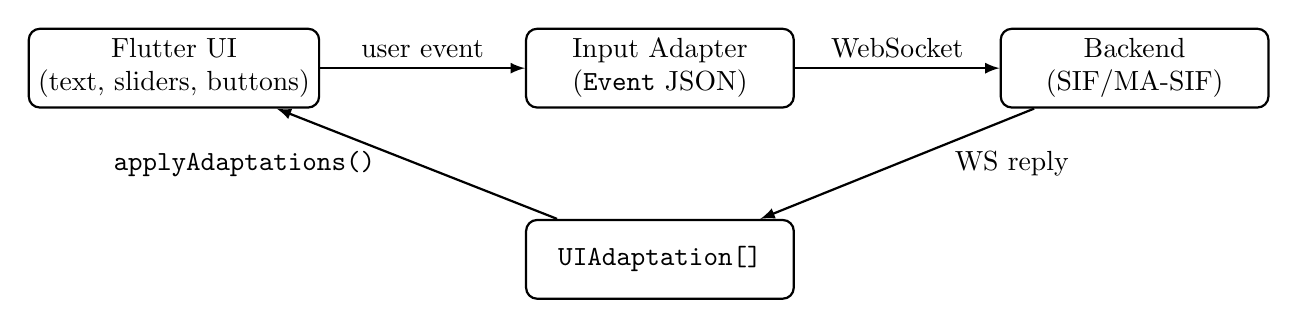
\begin{tikzpicture}[node distance=1.6cm,>=latex,rounded corners,thick]
\tikzstyle{box}=[draw, rounded corners, align=center, minimum width=3.4cm, minimum height=1.0cm]
\node[box] (ui) {Flutter UI\\(text, sliders, buttons)};
\node[box, right=2.6cm of ui] (adapter) {Input Adapter\\(\texttt{Event} JSON)};
\node[box, right=2.6cm of adapter] (backend) {Backend\\(SIF/MA-SIF)};
\node[box, below=1.4cm of adapter] (adapt) {\texttt{UIAdaptation[]}};
\draw[->] (ui) -- node[above]{user event} (adapter);
\draw[->] (adapter) -- node[above]{WebSocket} (backend);
\draw[->] (backend) -- node[right, xshift=6mm]{WS reply} (adapt);
\draw[->] (adapt) -- node[left,xshift=-4mm]{\texttt{applyAdaptations()}} (ui);
\end{tikzpicture}
\caption{Frontend data flow: events to adapter; adaptations back to UI.}
\label{fig:frontend_data_flow}
\end{figure}

\subsection{UI Composition \& State Model}
The UI is a scrollable list of device cards with minimalist controls each representing a smart home device such as a lamp, thermostat or a door. These cards contain core interactive elements, including buttons for on/off actions, sliders for settings such as temperature, and labels for contextual information. (Figure \ref{fig:ui_overview})

\begin{figure}[H]
\centering
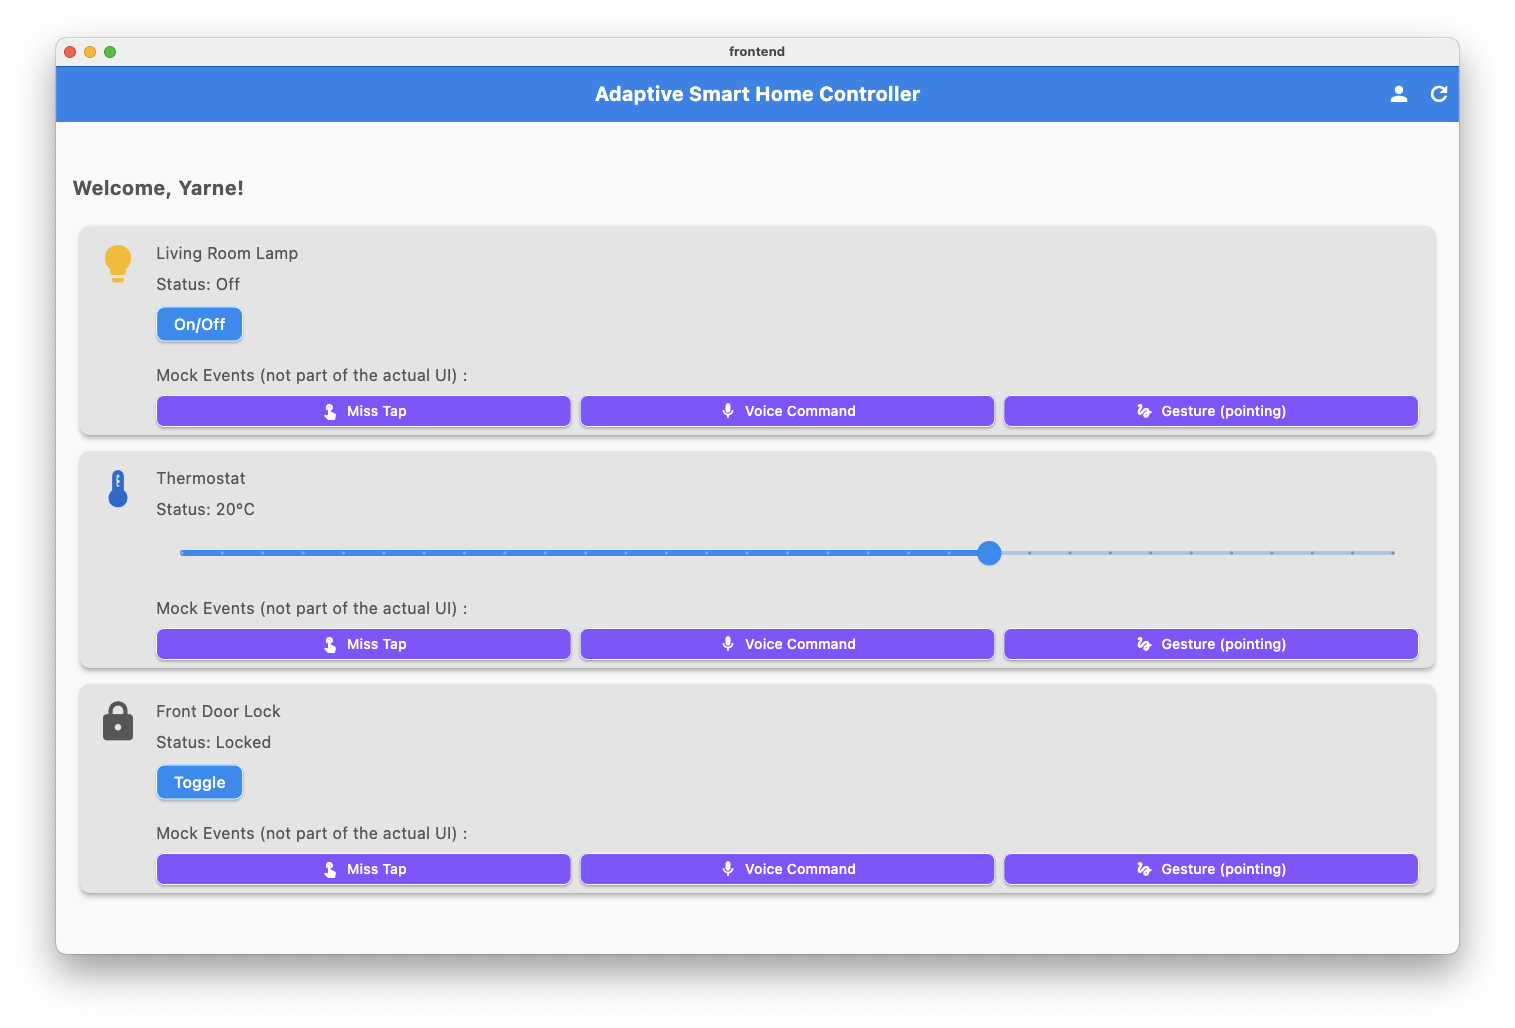
\includegraphics[width=.9\linewidth]{images/fig_ui_overview.png}
\caption{Smart Home Controller UI: scrollable device cards (Lamp, Thermostat, Lock) with minimalist controls and the mock event row (\emph{Miss Tap}, \emph{Voice Command}, \emph{Gesture}).}
\label{fig:ui_overview}
\end{figure}

The UI is intentionally minimalist, focusing on clarity and accessibility. Each device card (Lamp, Thermostat, Lock) presents its controls in a clean, uncluttered layout: large buttons for toggling states, sliders for adjustments, and concise status labels. The design prioritizes high visual contrast and generous spacing, making it easier for users with motor or visual impairments to interact. Adaptations such as increased button size, font scaling, or contrast changes are immediately reflected in the UI, with smooth animations to reinforce feedback. A persistent mock event row below each card allows users (or testers) to simulate miss-taps, voice commands, or gestures, demonstrating how the interface responds and adapts in real time. This modular structure ensures that accessibility enhancements are both visible and intuitive, supporting a wide range of user needs without overwhelming the interface.

\subsection{Event \& Adaptation Contract}
\label{sec:event_adaptation_contract}
\paragraph{Event (frontend$\rightarrow$backend).} Events carry modality and UI context:
\begin{lstlisting}[language=json, basicstyle=\ttfamily\small, caption={Event structure}]
{
  "eventType": "miss_tap", // e.g., touch, voice, gesture, miss_tap, ...
  "source": "touch", // modality
  "target": "lamp", // lamp | thermostat | lock
  "metadata": { "UI_element": "button" } // or slider, + command/gesture fields
}
\end{lstlisting}
\noindent\emph{Note.} The Dart \texttt{Event} uses camelCase fields (e.g., \texttt{eventType}, \texttt{targetElement}); the adapter serializes to snake\_case for the JSON contract.

This event will later be enriched with other required fields in the Input Adapter Layer, such as \texttt{timestamp} and \texttt{user\_id}.

\paragraph{Adaptation (backend$\rightarrow$frontend).} The backend replies with a list of atomic actions:
\begin{lstlisting}[language=json, basicstyle=\ttfamily\small, caption={Adaptation example actions}]
[
  { "action": "increase_button_size", "target": "lamp", "value": 1.2 },
  { "action": "increase_font_size", "target": "all",  "value": 1.15 },
  { "action": "increase_contrast", "target": "all" },
  { "action": "show_tooltip", "target": "lamp", "value": "Try a longer press" }
]
\end{lstlisting}

Adaptations received from the backend after being processed by the Input Adapter Layer are applied immediately using Flutter’s reactive state management, This is handled in the \verb|applyAdaptations(...)| callback function. For example, a \texttt{increase\_button\_size} action triggers an \texttt{AnimatedScale} widget update, enlarging the targeted button over a short animation to make the change more noticeable without disrupting the user’s flow. Similarly, a \texttt{increase\_contrast} action adjusts the application’s color scheme by updating theme parameters, while text-related adaptations update font sizes dynamically. Furthermore, when these adaptations reach the frontend, a brief highlight at the top of the application, indicates the changes being applied. This direct mapping between adaptation actions and Flutter widget properties allows the frontend to respond flexibly to a wide range of changes without requiring hardcoded layouts. See Table~\ref{tab:frontend-adapt-mapping} for details.

\begin{table}[H]
\centering
\caption{Adaptation-to-widget mapping (from \texttt{applyAdaptations}).}
\begin{tabular}{llp{7.8cm}}
\toprule
\textbf{Action} & \textbf{Target} & \textbf{Effect in UI} \\
\midrule
\texttt{increase\_button\_size} & device or \texttt{all} & Scales button via \texttt{buttonScales[target]} (animated). \\
\texttt{increase\_button\_border} & device or \texttt{all} & Doubles border thickness in \texttt{elementBorders}. \\
\texttt{increase\_slider\_size} & device or \texttt{all} & Multiplies slider scale in \texttt{sliderSizes}. \\
\texttt{increase\_font\_size} & (global) & Multiplies all entries in \texttt{fontSizes}. \\
\texttt{increase\_contrast} & (global) & Switches to high-contrast theme via \texttt{\_switchToHighContrastTheme()}. \\
\texttt{adjust\_spacing} & device or \texttt{all} & Scales spacing in \texttt{elementSpacing}. \\
\texttt{show\_tooltip} & device & Floating \texttt{SnackBar} with helper text. \\
\texttt{switch\_mode} & (global) & Records navigation-mode change (placeholder for future). \\
\texttt{trigger\_button} & lamp/lock & Toggles \texttt{deviceStatuses} (\emph{On/Off}, \emph{Locked/Unlocked}). \\
\texttt{simplify\_layout} & (global) & Sets \texttt{simplifiedLayout=true} to reduce clutter. \\
\bottomrule
\end{tabular}
\label{tab:frontend-adapt-mapping}
\end{table}

\subsection{Responsiveness \& Feedback}
While awaiting adaptations, the active card displays a rotating gradient border implemented via the \texttt{\_AnimatedGlowBorder} widget. This subtle animation serves as a visual indicator of system latency, signaling to users that their input is being processed and an adaptation is forthcoming. By using a non-intrusive glowing effect, the interface maintains user engagement without causing distraction or interrupting ongoing interactions (see Figure~\ref{fig:glow}). This approach is particularly beneficial for accessibility, as it provides clear feedback for users who may rely on visual cues to understand system status.
\begin{figure}[H]
\centering
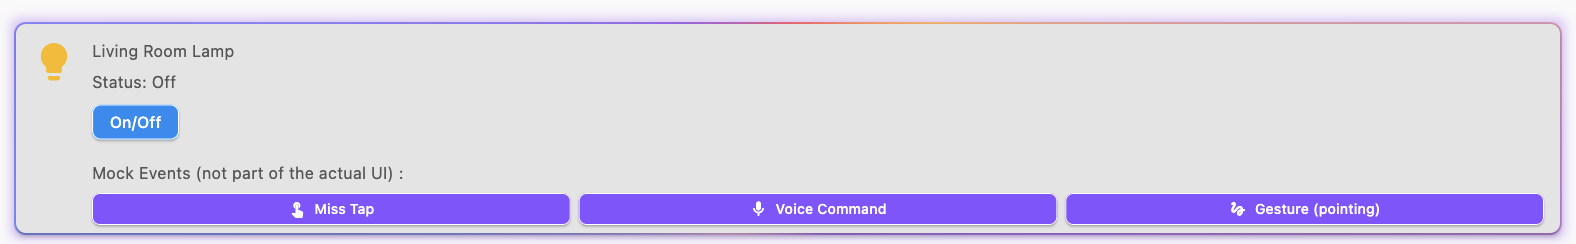
\includegraphics[width=1\linewidth]{images/fig_glow_border.png}
\caption{Loading indicator: rotating gradient card border while waiting for backend.}
\label{fig:glow}
\end{figure}

\subsection{Profile Bootstrap \& Editing}
On first run, the frontend checks if a profile exists; if not, it creates a default profile and persists it via the adapter. A bottom-sheet editor (\texttt{ProfileEditorSheet}) allows the ability to edit accessibility flags and UI preferences (font size, button size) of the user, see figure~\ref{fig:fig_profile_editor}, then calls \texttt{updateProfile(...)}.

\begin{lstlisting}[basicstyle=\ttfamily\small, caption={Profile initialization logic}]
if widget is initialized then
    adapter := AdaptiveUIAdapter(user_id, adaptation_callback)
    if adapter.checkProfile(user_id) then
        profile_data := adapter.getProfile(user_id)
        user_profile := parseProfile(profile_data)
    else
        user_profile := UserProfile(
            accessibility_needs=default,
            input_preferences=default,
            ui_preferences=default,
            interaction_history=[]
        )
        adapter.updateProfile(user_profile)
end if
\end{lstlisting}

\begin{figure}[H]
\centering
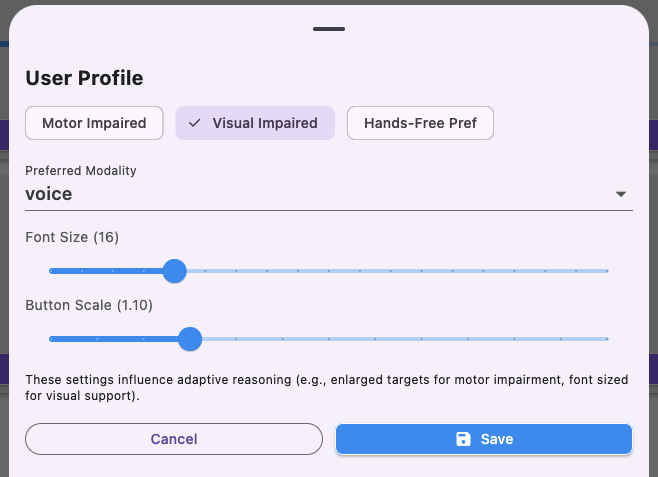
\includegraphics[width=.6\linewidth]{images/fig_profile_editor.png}
\caption{Profile editor for accessibility needs and UI preferences.}
\label{fig:fig_profile_editor}
\end{figure}

\subsection{Testing Harness: Mock Events \& Input Capture}
To validate the end-to-end pipeline without physical input hardware, a mock panel triggers \emph{miss tap}, \emph{voice command}, and \emph{gesture} events per device. Each button constructs an \texttt{Event} with modality, target, and UI context and sends it via \texttt{adapter.sendEvent(...)}. This keeps the architecture ready for real speech/gesture modules later, while staying reproducible for the study.

When a user presses on an mockup event in the test panel underneath each device, the frontend captures the event along with metadata such as the element’s type for UI context, the interaction type, and any relevant parameters. This data is sent through the Input Adapter Layer, which standardises the event into the framework’s JSON contract before forwarding it to the backend via WebSocket. The choice of WebSocket ensures that adaptations can be returned and applied in near real time, a critical requirement for maintaining a smooth user experience in accessibility scenarios. The power of the framework lies in the ability to set the \texttt{event\_type}, \texttt{source}, and others, dynamically based on user interactions, since the backend will use LLM-reasoning to interpret these events in context. While the fields are bound by the JSON contract to standardise events (for modularity and consistency), the actual values can be highly contextual and dynamic.

\textbf{Input Capture}: The frontend layer captures raw inputs from multiple modalities, including touch, voice, and gestures. Each modality is handled through specific Flutter widgets and event listeners:
\begin{itemize}
    \item \textbf{Touch}: Taps or miss-taps on buttons/sliders, detected via Flutter’s \verb|GestureDetector| or \verb|onPressed| callbacks. Miss-taps are mocked but extensible to hover or real misstap detection like \verb|MouseRegion| or \verb|Listener| widgets, to create a "detection bounding box".
    \item \textbf{Voice}: Commands like “Turn on lamp” or “Unlock door”, mocked for this thesis but extensible to libraries like \verb|speech_to_text| or Web Speech API.
    \item \textbf{Gestures}: Hand movements (e.g., point, swipe) via mock events, with future support for MediaPipe.
\end{itemize}

\subsection{Summary}
Overall, the Adaptive Smart Home Controller (\texttt{adaptive\_ui\_app.dart}) demonstrates how the frontend layer of the framework can be implemented in a way that is both platform-independent and responsive to dynamic adaptation instructions. By separating UI rendering from adaptation logic and using the Input Adapter Layer as a bridge, the application remains modular, making it easier to extend or replace individual components without affecting the overall system.

% implementation details and extensibility eye tracking
\section{Input Adapter (Dart): Transport, Serialization \& Adaptation Callback}
The adapter bridges the Flutter frontend and the SIF backend by (i) serializing internal \texttt{Event} objects into the JSON event contract, (ii) handling low-latency transport via WebSocket for adaptations, and (iii) managing user profiles over HTTP. This section focuses on the concrete implementation in \texttt{adaptive\_ui\_adapter.dart}: the class surface, serialization choices, transport lifecycle, and the \texttt{onAdaptations} callback function into the frontend. See Chapter~\ref{ch:chapter3} for the high-level event schema and field definitions.

\subsection{Class Overview}
\begin{figure}[H]
\centering
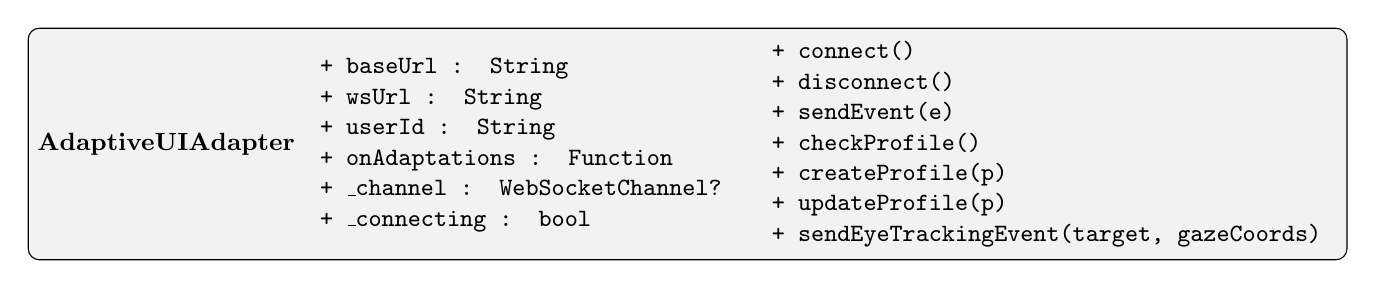
\begin{tikzpicture}[
    font=\small,
    class/.style={draw, rounded corners, fill=gray!10, minimum width=4.5cm, minimum height=2.2cm},
    attr/.style={font=\ttfamily\scriptsize},
    meth/.style={font=\ttfamily\scriptsize, text width=4.2cm, align=left}
]
\node[class] (adapter) {
    \textbf{AdaptiveUIAdapter}
    \vspace{2pt}
    \begin{tabular}{l}
        \texttt{+ baseUrl : String} \\
        \texttt{+ wsUrl : String} \\
        \texttt{+ userId : String} \\
        \texttt{+ onAdaptations : Function} \\
        \texttt{+ \_channel : WebSocketChannel?} \\
        \texttt{+ \_connecting : bool} \\
    \end{tabular}
    \vspace{2pt}
    
    \vspace{2pt}
    \begin{tabular}{l}
        \texttt{+ connect()} \\
        \texttt{+ disconnect()} \\
        \texttt{+ sendEvent(e)} \\
        \texttt{+ checkProfile()} \\
        \texttt{+ createProfile(p)} \\
        \texttt{+ updateProfile(p)} \\
        \texttt{+ sendEyeTrackingEvent(target, gazeCoords)} \\
    \end{tabular}
};

\end{tikzpicture}
\caption{Simplified UML-like diagram for \texttt{AdaptiveUIAdapter}.}
\label{fig:adaptive-ui-adapter}
\end{figure}

In the current implementation (Figure~\ref{fig:adaptive-ui-adapter}), the adapter intercepts mock events generated by the frontend, such as missed button presses, missed slider adjustments, or simulated voice commands. Each event is enriched with metadata, including the user’s identifier, a timestamp, the type of interaction, and any target element references. The adapter then converts this information into the JSON event contract, further defined in Chapter~\ref{ch:chapter3}, which serves as the standard interface between the frontend and backend. This contract includes fields for event type, source modality, target element, coordinates if applicable, confidence level, time stamp, user\_id and additional metadata such as the spoken command in the case of voice input.

\subsection{Internal Representations of Event, Adaptation and User Profiles}
The adapter defines core Dart classes for representing interaction events, user profiles, and adaptation actions. The \texttt{Event} class encapsulates all relevant fields such as event type, source modality, target element, etc., ensuring every interaction is consistently structured and easily serializable to the backend’s JSON contract (see figure \ref{fig:adapter-classes} for schema details). Similarly, \texttt{UIAdaptation} models adaptation instructions received from the backend, while \texttt{UserProfile} maintains accessibility needs, preferences, and recent history. These unified data structures guarantee reliable, type-safe communication between frontend and backend, simplify integration, and support extensibility for future modalities or adaptation types.

\begin{figure}[H]
\centering
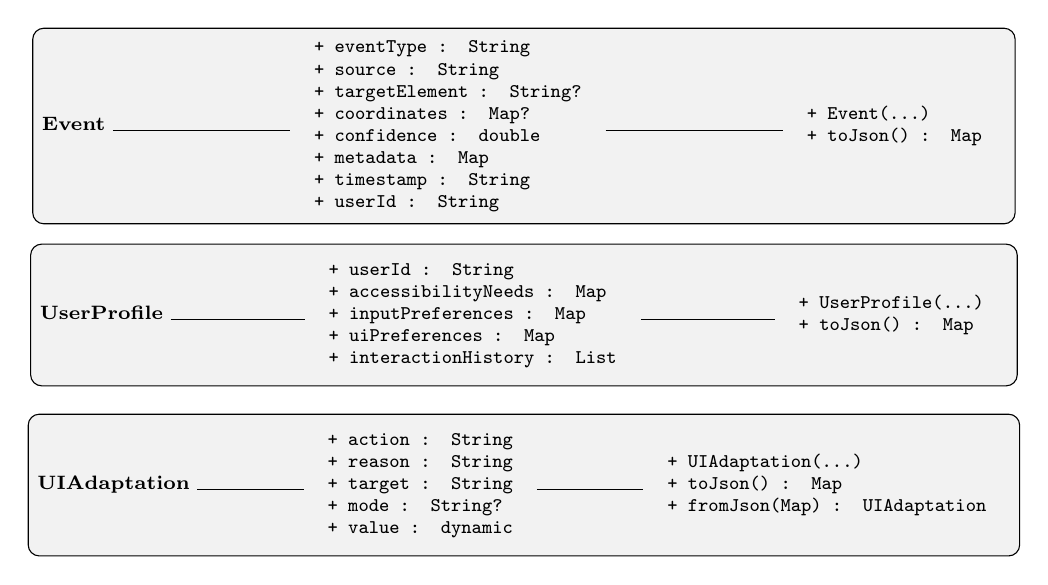
\begin{tikzpicture}[
    scale=0.6, % reduced from 0.8 for smaller diagram
    font=\scriptsize,
    class/.style={draw, rounded corners, fill=gray!10, minimum width=3cm, minimum height=1.8cm, align=left},
    attr/.style={font=\ttfamily\tiny},
    meth/.style={font=\ttfamily\tiny}
]

% Event class
\node[class] (event) at (0,0) {
    \textbf{Event}
    \rule{2.25cm}{0.3pt}
    \begin{tabular}{l}
        \texttt{+ eventType : String} \\
        \texttt{+ source : String} \\
        \texttt{+ targetElement : String?} \\
        \texttt{+ coordinates : Map?} \\
        \texttt{+ confidence : double} \\
        \texttt{+ metadata : Map} \\
        \texttt{+ timestamp : String} \\
        \texttt{+ userId : String} \\
    \end{tabular}
    \rule{2.25cm}{0.3pt}
    \begin{tabular}{l}
        \texttt{+ Event(...)} \\
        \texttt{+ toJson() : Map} \\
    \end{tabular}
};

% UserProfile class
\node[class] (profile) at (0,-4) {
    \textbf{UserProfile}
    \rule{1.7cm}{0.3pt}
    \begin{tabular}{l}
        \texttt{+ userId : String} \\
        \texttt{+ accessibilityNeeds : Map} \\
        \texttt{+ inputPreferences : Map} \\
        \texttt{+ uiPreferences : Map} \\
        \texttt{+ interactionHistory : List} \\
    \end{tabular}
    \rule{1.7cm}{0.3pt}
    \begin{tabular}{l}
        \texttt{+ UserProfile(...)} \\
        \texttt{+ toJson() : Map} \\
    \end{tabular}
};

% UIAdaptation class
\node[class] (adaptation) at (0,-7.6) {
    \textbf{UIAdaptation}
    \rule{1.35cm}{0.3pt}
    \begin{tabular}{l}
        \texttt{+ action : String} \\
        \texttt{+ reason : String} \\
        \texttt{+ target : String} \\
        \texttt{+ mode : String?} \\
        \texttt{+ value : dynamic} \\
    \end{tabular}
    \rule{1.35cm}{0.3pt}
    \begin{tabular}{l}
        \texttt{+ UIAdaptation(...)} \\
        \texttt{+ toJson() : Map} \\
        \texttt{+ fromJson(Map) : UIAdaptation} \\
    \end{tabular}
};

\end{tikzpicture}
\caption{High-level class diagram for Input Adapter Layer data structures.}
\label{fig:adapter-classes}
\end{figure}

\subsection{Transport \& Profile Management}
Before forwarding an event, the adapter queries the backend via HTTP to check whether a profile exists for the given user. If no profile is found, it prompts the frontend to initiate a profile creation request, using default parameters or pre-filled accessibility preferences where available. This mechanism prevents situations where adaptation requests are processed without the necessary user context, which could lead to ineffective or even counterproductive UI changes.

Communication with the backend is handled primarily through WebSocket for low-latency adaptation feedback. HTTP requests are used for profile management, batch operations, and other non-real-time interactions. This division ensures that profile updates and administrative tasks do not interfere with the responsiveness of live adaptations, see table \ref{tab:adapter_endpoints} for details.

\begin{table}[H]
\centering
\caption{Adapter endpoints used by \texttt{adaptive\_ui\_adapter.dart}.}
\begin{tabular}{lll}
\toprule
Purpose & Method/Proto & Path \\
\midrule
Realtime adaptations & WebSocket & \verb|/ws/adapt| \\
Check profile exists & GET & \verb|/profile/{user_id}| \\
Create profile       & POST & \verb|/profile| \\
Update profile       & POST  & \verb|/profile| \\
\bottomrule
\end{tabular}
\label{tab:adapter_endpoints}
\end{table}
\newpage
\textbf{WebSocket Lifecycle \& Error Handling:}
\begin{figure}[H]
\centering
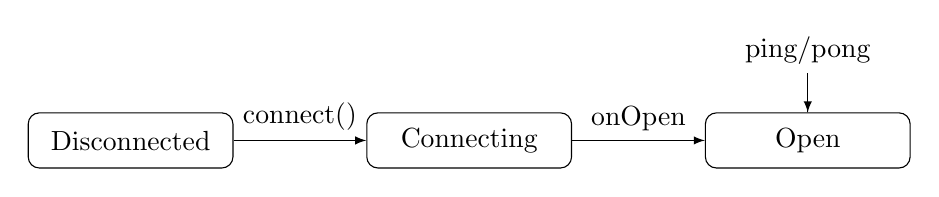
\begin{tikzpicture}[>=latex, node distance=1.8cm, on grid, auto,
  state/.style={draw, rounded corners, align=center, minimum width=2.6cm, minimum height=7mm}]
\node[state] (disc) {Disconnected};
\node[state, right=of disc,xshift=25mm] (conn) {Connecting};
\node[state, right=of conn, xshift=25mm] (open) {Open};

\draw[->] (disc) -- node{connect()} (conn);
\draw[->] (conn) -- node{onOpen} (open);

\draw[->] (open) .. controls +(0,1.0) and +(0,1.0) .. node[above]{ping/pong} (open);
\end{tikzpicture}
\caption{Adapter WebSocket lifecycle with reconnect backoff.}
\end{figure}

\noindent In \texttt{adaptive\_ui\_adapter.dart}:
\begin{itemize}
  \item On \textbf{open}: subscribe to messages and (optionally) flush any queued events.
  \item On \textbf{message}: parse JSON array/object, convert to \texttt{UIAdaptation} list, invoke \texttt{onAdaptations}.
  \item On \textbf{error/done}: close channel.
  \item \textbf{Keep-alive via ping/pong}: Keep-alive via ping/pong is handled at the protocol level; the adapter does not send explicit pings.
\end{itemize}

\textbf{Sending Events:}

When the frontend is ready to send an event, it calls the \texttt{sendEvent} function from the adapter, which enriches the event data with metadata (e.g., user\_id, timestamp), serializes it into JSON, and sends it over the WebSocket connection. 

\begin{lstlisting}[language=Dart,basicstyle=\ttfamily\small,caption={sendEvent: serialize and send over WS}]
void sendEvent(Event eventData) {
    eventData.timestamp = DateTime.now().toIso8601String();
    eventData.userId = userId;
    channel!.sink.add(jsonEncode(eventData.toJson()));
}
\end{lstlisting}

\textbf{Receiving Adaptations:}

When the adapter receives adaptations from the backend in the WebSocket channel, the adapter processes the JSON and converts them in a \texttt{UIAdaptation} list. This list is then passed to the \texttt{onAdaptations} frontend callback function. This function is responsible for updating the UI based on the received adaptation data, see Section~\ref{sec:event_adaptation_contract} for more details on this process.

\textbf{Profile Management:}

Profile management is mostly done by the frontend, with the Input Adapter Layer providing all the necessary functions and ensuring that every user interaction is contextualized with the correct accessibility preferences and history. Before sending any event to the backend, the frontend (as described earlier) checks whether a profile exists for the current user by calling \texttt{checkProfile()}. If no profile is found, it creates one using \texttt{createProfile(UserProfile p)}, which serializes the profile data and posts it to the backend. Updates to the profile, such as changes in accessibility needs or UI preferences, are handled by \texttt{updateProfile(UserProfile p)}, which issues a POST request with the updated profile JSON. These functions guarantee that the backend always receives events enriched with up-to-date user context, supporting personalised adaptation and continuous learning.

\subsection{Extensibility Example}
As proof-of-concept for the extensibility of the framework, a gaze event hook was implemented that incorporates eye-tracking data into an event. This demonstrates how easily new input modalities can be integrated into the existing architecture.
\begin{lstlisting}[language=Dart,basicstyle=\ttfamily\small,caption={Gaze event hook (testing harness)}]
void sendEyeTrackingEvent(String target, Map<String,double> gazeCoords) {
  sendEvent(Event(
    eventType: 'eye_tracking',
    source: 'gaze',
    targetElement: target,
    coordinates: gazeCoords,
    confidence: 1.0,
  ));
}
\end{lstlisting}
\textit{Note:} This can either be done in the frontend or directly in the adapter, depending on the specific requirements of the application. For demonstration purposes, the gaze event hook was implemented in the adapter, while the frontend would be a more logical place for it in a production setting.

\subsection{Summary}
The adapter is fully wired for touch events and for mocked voice/gesture events triggered from the frontend’s test panel, enabling end-to-end validation without external hardware. The adapter treats mocked and real events identically, so integrating actual speech/gesture modules later is a frontend-only change. By isolating serialization, profile checks, and transport here, the frontend stays focused on rendering, and the backend receives consistent inputs. The same adapter design can be reused in SwiftUI or other platforms with minimal changes to the method surface and JSON contract.

\section{SIF Backend Layer: Implementation of Adaptation Logic}
The backend implements the decision‑making core of the framework. It receives standardised events from the adapter, fuses them with user profiles and recent interaction history, and returns concrete adaptation actions for the frontend to apply. The service is written in Python using FastAPI, with Uvicorn for serving requests and MongoDB for persistent storage of profiles and logs. WebSocket is used for low‑latency, bidirectional communication during interaction, HTTP is used for profile management and auxiliary endpoints.

\subsection{Webserver layout and endpoints}
The application exposes a WebSocket endpoint, \texttt{/ws/adapt}, that accepts JSON events matching the contract introduced earlier. Each message is parsed into a Pydantic \texttt{Event} model, the user profile is loaded from MongoDB, and the event, profile, and short history window are passed to the Smart Intent Fusion routine. The resulting adaptation list is returned on the same socket, allowing the frontend to update the UI immediately. For non‑interactive operations the backend offers \texttt{POST /profile} for profile creation, \texttt{GET /profile/{user\_id}} for retrieval, and a small set of diagnostic endpoints such as \texttt{GET /full\_history} and \texttt{GET /modalities}. Profile writes use FastAPI \texttt{BackgroundTasks}, which keeps the interaction path responsive while updates are persisted asynchronously.

\subsubsection*{Startup \& Runtime}
For local runs, the service is started via a small shell script (\texttt{start\_backend\_processes.sh}) that prepares a venv, checks MongoDB, and runs Uvicorn with explicit WebSocket keepalive settings:
\begin{lstlisting}[basicstyle=\ttfamily\small,caption={Backend startup (excerpt)}]
uvicorn backend:app --reload --host 0.0.0.0 --port 8000 \
  --ws websockets --ws-ping-interval 60 --ws-ping-timeout 180
\end{lstlisting}
This configuration enables reliable long-lived WS sessions during interactive testing, and eases startup of all the different services.

\subsection{Data persistence and history management}
MongoDB stores user profiles in a \texttt{profiles} collection and event–adaptation pairs in a \texttt{logs} collection. Profiles are indexed by \texttt{user\_id} to allow direct lookups during interaction. Each time an event is processed the backend appends a compact JSON representation to the profile’s \texttt{interaction\_history}, capped to a small sliding window. This keeps the prompt context focused on recent behaviour while avoiding unnecessary growth in the database. For redundancy, a JSONL file mirrors the log entries during development, which simplifies offline inspection or debugging purposes when the database is reset.

\subsection{Smart Intent Fusion and MA‑SIF}
The fusion step supports two paths. A multi‑agent configuration, MA‑SIF, is the default. It loops over a set of specialised LLM agents, UI, Geometry, and Input, each prompted with the current event, the user profile, and a short history via runtime injection (for more details see Chapter~\ref{ch:chapter4}), defined in the \texttt{sif\_config.json}. These agents propose structured adaptations in their domain, for example increasing button size, adjusting spacing, switching input mode, or triggering a button when intent is clear. Their outputs are then passed to a dedicated Validator agent that consolidates, filters, and normalises the suggestions into a final list. The validator removes duplicates, corrects out‑of‑range values, and ensures that every adaptation conforms to the allowed action set and includes a target and either a value or a mode and more. See Table~\ref{fig:current-agent-configuration} for the current agent configuration.

A single‑agent SIF path is also available. It produces a complete adaptation list in one call and is useful when quick iteration is preferable over agent specialisation. Both paths share the same I/O schema, which keeps the frontend indifferent to which reasoning strategy is currently set to active.

\subsubsection*{Current Agent Configuration (MA-SIF balanced) (from \texttt{sif\_config.json})}
\begin{table}[H]
\centering
\begin{tabular}{p{2.1cm}p{4cm}p{4cm}p{4cm}}
\toprule
\textbf{Agent} & \textbf{Focus (examples)} & \textbf{Allowed actions} & \textbf{Model / params} \\
\midrule
UI suggestion & increase font sizes; enable contrast mode; stronger button borders; tooltips & \texttt{increase\_font\_size}, \texttt{increase\_contrast}, \texttt{increase\_button\_border}, \texttt{show\_tooltip} & \texttt{gemini-2.5-flash-lite}, temp{=}0.2, timeout{=}15\,s, thinking\_budget=0 \\
Geometry & spacing; button size; slider size; simplify layout & \texttt{increase\_button\_size}, \texttt{increase\_slider\_size}, \texttt{adjust\_spacing}, \texttt{simplify\_layout} & \texttt{gemini-2.5-flash-lite}, temp{=}0.2, timeout{=}15\,s, thinking\_budget=0 \\
Input & mode switching; trigger buttons & \texttt{switch\_mode}, \texttt{trigger\_button} & \texttt{gemini-2.5-flash-lite}, temp{=}0.2, timeout{=}15\,s, thinking\_budget=0 \\
Validator & consolidate + validate all suggestions & \emph{all actions above} & \texttt{gemini-2.5-flash}, temp{=}0.3, timeout{=}30\,s, thinking\_budget=-1 \\
\bottomrule
\end{tabular}
\caption{MA\textendash SIF agents, focus, allowed actions, and model settings (runtime configurable).}
\label{fig:current-agent-configuration}
\end{table}

\paragraph{Runtime defaults:}
\begin{itemize}
  \item \textbf{Default model settings:} 
    \begin{itemize}
        \item UI/Geometry/Input use \texttt{gemini-2.5-flash-lite} with a temperature of 0.2, a 15\,s timeout and thinking budget of 0 (no thinking).
        \item Validator uses \texttt{gemini-2.5-flash} with a temperature of 0.3, a 30\,s timeout and thinking budget of -1 (dynamic).
    \end{itemize}
  \item \textbf{Whitelisting:} Each agent is restricted to an \emph{allowed action set}; Validator allows the union set only.
  \item \textbf{Schema enforcement:} Responses must match the JSON schema (\texttt{response\_json\_schema}); non-conforming replies trigger fallback.
  \item \textbf{Low temperature + narrow prompts:} Specialist prompts reduce creative drift and injection surface.
  \item \textbf{Timeouts:} Per-agent time budgets ensure the loop returns within interaction thresholds.
\end{itemize}
\newpage

\subsection{LLM invocation (Gemini)}
For each event, the backend invokes Gemini per specialist agent (UI, Geometry, Input) and then once for the Validator, in sequence. Each call is single-shot (no streaming) with a strict JSON response contract. Requests are composed as follows:

\paragraph{Request composition:}
\begin{itemize}
  \item \textbf{Context blocks}: \texttt{event\_json}, \texttt{profile\_json} (accessibility flags, preferences), and \texttt{history\_json} (recent 10 interactions). These are injected into the Agent's prompt at runtime, as mentioned earlier.
  \item \textbf{Agent preamble}: a short, role-specific instruction and focus items plus an explicit \emph{allowed action set} (whitelisting).
  \item \textbf{Output contract}: instructed to return only a JSON envelope \texttt{\{"adaptations":[...]\}} (no prose).
\end{itemize}

\paragraph{Generation configuration (per call).}
\begin{itemize}
  \item \textbf{Model/temperature}: UI, Geometry, Input use \texttt{gemini-2.5-flash-lite} at $T{=}0.2$; the Validator uses \texttt{gemini-2.5-flash} at $T{=}0.3$ (see \texttt{sif\_config.json}).
  \item \textbf{Response format}: \texttt{response\_mime\_type=application/json} with a \textbf{JSON Schema} that enforces types, fields, and that either \texttt{value} (numeric) \emph{or} \texttt{mode} (categorical) is present.
  \item \textbf{Budgets}: per-agent timeout $\approx$ 15\,s; Validator timeout $\approx$ 30\,s. Calls are sequential by design to keep rate-limits predictable and simplify partial results.
  \item \textbf{Determinism}: low temperatures, single candidate, narrow prompts; agents propose domain-scoped adaptations, Validator consolidates/filters to the final set.
\end{itemize}

\paragraph{Failure handling.}
If a specialist agent times out or returns invalid JSON, its suggestions are omitted; the Validator runs on whatever is available. If validation still fails schema checks or time outs, the backend emits the available adaptation or conservative rule-based adaptations as a fallback.

\subsection{Structured outputs and guardrails}
To reduce hallucinations and schema drift, the backend requests JSON‑typed responses from the LLM with an explicit schema and allowed actions, as described earlier in Chapter~\ref{ch:chapter4}. The prompt defines required fields, expected types, and a one‑of constraint that demands either a numeric \texttt{value} or a categorical \texttt{mode}. Agent prompts are intentionally narrow, which improves determinism. The validator prompt is broader, since it must adjust conflicting suggestions and justify final choices. Despite these controls, invalid outputs still occur occasionally. However, the schema can be enforced at two distinct levels: by the agents and by the validator. This dual-level approach makes it easier for the validator to ensure that the agents' adaptations are compliant. Furthermore, it has a defensive layer that falls back to simple rules if all LLM validation fails.
The output schema will produce an adaptation of the following format:
\begin{lstlisting}[language=json,basicstyle=\ttfamily\small,caption={Example adaptation Format}]
{"adaptations":[{"action":"...","target":"...","value":1.2,"mode":"...","reason":"...","intent":"..."}]}
\end{lstlisting}

\subsection{Rule‑based fallback and resilience}
A lightweight rule engine acts as a safety net when LLM calls time out or the provider is unavailable. This rule engine comes into action when all the suggestion agents fail (no output). It covers essential accessibility behaviours, for example increasing button size after a miss‑tap, switching to voice for users flagged as motor‑impaired, or enabling high‑contrast mode for visually impaired profiles. These rules are intentionally conservative, they guarantee progress without surprising the user, and they keep the implementation usable in environments with unstable connectivity.

\subsubsection*{Fallback rules (summary)}
\begin{table}[H]
\centering
\caption{Rule triggers and conservative adaptations (fallback path).}
\begin{tabular}{p{5.7cm}p{9.2cm}}
\toprule
\textbf{Trigger} & \textbf{Adaptation(s)} \\
\midrule
Miss tap (\texttt{event\_type="miss\_tap"}) or slider miss & \texttt{increase\_button\_size} on target (default \texttt{1.3}); intent=``difficulty hitting target''. \\
Profile indicates motor impairment & \texttt{increase\_button\_size} on \texttt{all}; intent=``Improve accessibility''. \\
Profile indicates visual impairment & \texttt{increase\_contrast} on \texttt{all}; intent=``improve visibility''. \\
Voice command detected (\texttt{event\_type="voice"}) & \texttt{switch\_mode} to \texttt{voice} on \texttt{all}. \\
\bottomrule
\end{tabular}
\end{table}

\subsection{Heatmap Analysis}
Due to time constraints, heatmap analysis is not implemented. This is a potential area for future work, as understanding user interaction patterns and frequent touch points, could further enhance the system's adaptability. Heatmap analysis has a big potential in the repositioning of UI elements based on the heatmap data, this could improve accessibility for users with specific needs like gesture-based inputs. Since the repositioning of elements is not supported in this first iteration, the focus remains on immediate adaptation strategies, which made heatmap analysis out of scope.

\subsection{Latency, partial results, and error handling}
The WebSocket loop is designed to return something useful as quickly as possible. Agent calls run in sequence within short time budgets. If one agent fails to respond, the validator operates on the remaining suggestions rather than waiting indefinitely. The backend aims to keep per‑event processing below the threshold where users notice a lag on interaction, which is important for accessibility, particularly when enlarging targets immediately after an error. In practice, most adaptations are returned quickly by the smaller suggestion agents, while validation can become the slowest step in complex scenes. When validation exceeds its budget the backend returns the best available subset, then continues to append the event to the user’s history so future interactions benefit from the context.

\subsection{Security and CORS considerations}
During development the backend enables permissive CORS to simplify local testing across platforms. Profiles are keyed by \texttt{user\_id} rather than personal data. For production deployment, stricter origins, authentication, and encryption would be required. These measures are outside the scope of this prototype, but the separation of concerns in the current design makes them straightforward to add.

\subsection{Summary}
In its current form the backend delivers a complete adaptation pipeline: events arrive over WebSocket, profiles and short history windows are loaded from MongoDB, MA-SIF produces structured suggestions, a validator consolidates them, and the result is returned to the frontend within a single interaction loop. When LLM reasoning is unavailable, conservative rules ensure the interface remains usable. This combination of multi‑agent reasoning, strict schemas, and rule-based fallbacks gives the system both flexibility and reliability, which is essential for accessibility‑focused adaptations.

\section{User Profile and Context Implementation}
The user profile and context subsystem was implemented as a dedicated data service in the SIF backend, designed to persist accessibility needs, interaction preferences, baseline UI configurations, and a capped history of recent events. MongoDB serves as the primary storage layer, with the \texttt{profiles} collection indexed on \texttt{user\_id} as described earlier for constant-time retrieval during event processing.

When a new event is received via the WebSocket (\texttt{/ws/adapt}), the backend queries the profile store using the supplied \texttt{user\_id}. If no profile exists, the profile will be created and added to the MongoDB using \texttt{insert\_one} before continuing, otherwise the profile will be retrieved using \texttt{find\_one} or updated using \texttt{update\_one}, ensuring that all adaptation decisions are made in a contextualized environment. This retrieval step is synchronous, guaranteeing that the most recent committed profile is available to the reasoning pipeline before any LLM or rule-based evaluation occurs. Interaction history is maintained using MongoDB’s \texttt{\$push} with \texttt{\$slice} operators to append the incoming event while capping the array length at 10 entries for efficiency. This rolling history provides the SIF agents with temporal context, enabling progressive personalization; for example, recognising a pattern of repeated miss-taps and proactively switching to voice mode. Updates to the history are performed asynchronously to avoid blocking real-time adaptation.

Profile documents are structured as JSON as described in Chapter~\ref{ch:chapter4}, containing four key sections: \texttt{accessibility\_needs} (boolean capability flags), \texttt{input\_preferences} (preferred modality and fallback order), \texttt{ui\_preferences} (default font size, button scale and more), and \texttt{interaction\_history} (recent event log). This schema strikes a balance between simplicity and extensibility, allowing new fields to be added without migration overhead.

To optimise performance and safety, all profile mutations are atomic, relying on MongoDB transactions to prevent race conditions when simultaneous events and updates occur. Adaptation logs are stored separately in the \texttt{logs} collection and mirrored to a local \texttt{adaptation\_log.jsonl} file, supporting offline analysis and reproducibility of evaluation results. Furthermore, if a profile update is in-flight during an event, the backend uses the latest committed profile, mitigated by client-side checks (waiting for \texttt{POST /profile} success) and server-side transactions.

This implementation ensures that every adaptation decision, whether produced by a static rule or the multi-agent LLM pipeline, is grounded in the user’s persisted profile and immediate interaction context, enabling consistent, personalised, and stateful UI behaviour across sessions.

\section{Dynamic Adaptation Mechanisms Implementation}
The dynamic adaptation mechanism is the final stage in the adaptation pipeline, where decisions made by the backend are translated into immediate and visible changes in the user interface. In the current implementation, this process is tightly integrated with Flutter’s reactive widget system, allowing adaptation actions to be applied without forcing full UI rebuilds or navigation resets.

When the backend sends an adaptation list over the WebSocket connection, the frontend parses each action and routes it to the relevant UI element. Actions are defined in the strict JSON schema described earlier, containing the \texttt{action} type, a \texttt{target} identifier, a \texttt{value} or \texttt{mode}, and a human-readable \texttt{reason} and \texttt{intent} it inferred from the adaptation. This standardisation allows the same adaptation handler to process diverse actions without requiring modality-specific logic.

The framework applies a predefined set of accessibility-oriented actions (see Table~\ref{tab:frontend-adapt-mapping} for the concrete widget mappings used by the Flutter implementation).
These adaptation actions form the cornerstone of the framework’s accessibility-driven approach, addressing diverse user needs in the Adaptive Smart Home Controller. Each action is carefully designed to align with WCAG 2.1 guidelines, ensuring inclusivity for motor-impaired users (e.g., larger buttons/sliders, increased spacing), visually impaired users (e.g., high-contrast modes, highlighted borders), and hands-free users (e.g., tooltips, mode switching).

\subsection{Application Mechanics (State, Animation, Ordering)}
\begin{itemize}
  \item \textbf{State deltas.} Element-scoped actions update per-element maps (e.g., \texttt{buttonScales[target]}, \texttt{elementBorders[target]}), while global actions flip flags or theme variables (\texttt{increase\_contrast}, \texttt{switch\_mode}).
  \item \textbf{Animation semantics.} Size and spacing changes use lightweight implicit animations (\texttt{AnimatedScale}, \texttt{AnimatedContainer}) with short durations to make changes perceivable without disrupting interaction.
  \item \textbf{Ordering.} Adaptations are applied in the order received; the backend validator guarantees a coherent, non-overlapping set. On receipt, the active card’s glow border stops and controls are re-enabled.
\end{itemize}

The application of adaptations begins with a lookup to determine whether the \texttt{target} element exists in the current view. If it does, the corresponding widget state is updated directly. For example, an \texttt{increase\_button\_size} action adjusts the scale factor property of the button widget, and an \texttt{increase\_font\_size} action updates the text style parameter. Where appropriate, changes are animated using Flutter’s \texttt{AnimatedScale} or \texttt{AnimatedContainer} to make the transition noticeable without distracting the user. This animation step is particularly important for accessibility, as it helps the user understand that the interface has been modified intentionally. The loading indicator displayed around the card being interacted is now also triggered to stop playing.

Adaptations that affect the entire interface, such as \texttt{increase\_contrast} or \texttt{switch\_mode}, are handled at the application theme level. Contrast adjustments update the color palette by replacing the primary and background colors with higher-contrast alternatives, while mode switches alter the active input modality, for example switching from touch to voice. These global changes are propagated across all widgets automatically through Flutter’s state management, ensuring consistency without manually updating each element (see table~\ref{tab:adaptation-scope} for an overview).

\begin{table}[H]
\centering
\caption{Scope of adaptations in the Flutter implementation.}
\begin{tabular}{lp{9cm}}
\toprule
\textbf{Global (theme/state)} & \texttt{increase\_contrast}, \texttt{switch\_mode}, \texttt{simplify\_layout}, \texttt{increase\_font\_size (all)} \\
\midrule
\textbf{Element-scoped} & \texttt{increase\_button\_size}, \texttt{increase\_button\_border}, \texttt{increase\_slider\_size}, \texttt{adjust\_spacing}, \texttt{show\_tooltip}, \texttt{trigger\_button} \\
\bottomrule
\end{tabular}
\label{tab:adaptation-scope}
\end{table}

Not all adaptations are implemented with live modality inputs. For demonstration purposes, actions triggered by voice or gesture events are generated from simulated events in the frontend’s test panel in each device card, like was mentioned earlier. However, these simulated actions follow the same processing path as real events, which means that integrating actual input sources in the future will require no changes to the adaptation mechanism itself.

\subsection{Conflicts and Unknown Actions}
The validator resolves conflicts server-side; the frontend applies the resulting set atomically in a single frame. If duplicate actions target the same element, the last write wins within the frame. Unknown or ill-typed actions are logged and ignored, preserving UI stability.

\subsection{Real-Time Adaptation Example}
To illustrate the framework's adaptation capabilities, consider a scenario where a visually impaired user with voice preference attempts to interact with the Smart Home Controller. The user profile contains the following settings:

\begin{lstlisting}[language=json, caption={User profile for visually impaired user, shortened}]
{
    ...
    "accessibility_needs": { "visual_impaired": true },
    "input_preferences": { "preferred_modality": "voice" },
    "ui_preferences": { "font_size": 16, "button_scale": 1.1 }
}
\end{lstlisting}

\paragraph{Event Trigger:} The user attempts to activate the lamp by tapping its button but misses the target due to the button's insufficient size relative to their visual and motor coordination needs. This generates a \texttt{miss\_tap} event on the \texttt{lamp} target, which is captured by the frontend and sent through the Input Adapter Layer to the SIF backend.

\paragraph{SIF Reasoning Process:} The backend combines the miss-tap event with the user's profile and recent interaction history. The MA-SIF agents analyze the situation:
\begin{itemize}
        \item \textbf{UI Agent:} Recognizes visual impairment flags and suggests contrast and font improvements
        \item \textbf{Geometry Agent:} Identifies the miss-tap pattern and recommends button enlargement and border enhancement
        \item \textbf{Input Agent:} Notes voice preference and triggers the intended action while suggesting mode awareness
        \item \textbf{Validator Agent:} Consolidates suggestions and ensures compatibility
\end{itemize}

\paragraph{Adaptation Response:} The backend returns five coordinated adaptations:
\begin{enumerate}
    \item \textbf{Font size increase (lamp):} Scale text by 1.2× for better readability given visual impairment
    \item \textbf{Button size increase (lamp):} Enlarge the lamp button by 1.2× to reduce future miss-taps
    \item \textbf{Contrast enhancement (global):} Switch to high-contrast mode across the entire interface
    \item \textbf{Button border enhancement (lamp):} Strengthen the lamp button border for better visual definition
    \item \textbf{Direct button activation (lamp):} Trigger the lamp immediately via voice command, fulfilling the user's intent despite the miss-tap
\end{enumerate}
\paragraph{Validator Agent Reasoning:} The Validator accepted all (5 out of 5) adaptations from the suggestion agents, following this reasoning:
\begin{itemize}
    \item \textbf{Font size increase (lamp):} User has visual impairment and has previously missed taps on the lamp button, suggesting difficulty in seeing the target.
    \item \textbf{Contrast enhancement (global):} User has visual impairment, and increasing contrast can improve visibility of UI elements.
    \item \textbf{Button border enhancement (lamp):} User has visual impairment and has previously missed taps on the lamp button, suggesting difficulty in accurately targeting the button.
    \item \textbf{Button size increase (lamp):} The user has a visual impairment and has recently missed tapping the lamp button twice. Increasing the button size will make it easier to interact with.
    \item \textbf{Direct button activation (lamp):} User has repeatedly missed tapping the lamp button, indicating a potential difficulty with precise touch interactions. The current miss-tap command to turn on the lamp suggests a preference for hands-free operation. Triggering the button via voice command is a suitable adaptation.
\end{itemize}

\paragraph{Visual Impact:} 
The transformation (see figure \ref{fig:before-after-adaptation}) demonstrates the framework's accessibility-focused approach. The originally small lamp button (standard size) becomes significantly more prominent through size scaling and border enhancement. Text elements throughout the interface are enlarged to improve readability, while the high-contrast theme ensures better visibility for users with visual impairments. The lamp is also activated immediately, fulfilling the user's original intent despite the initial miss-tap.

\paragraph{Personalization Benefits:} 
This example illustrates how the framework moves beyond generic accessibility settings to deliver contextual, profile-aware adaptations. Rather than applying a one-size-fits-all solution, the system combines the user's declared visual impairment with their interaction behavior (miss-tap) and stated preferences (voice modality) to produce a coordinated set of improvements that address both immediate needs (completing the lamp activation) and future interactions (persistent size and contrast improvements).
The adaptation occurred within the framework's typical latency range ($\sim$13 seconds median), allowing the user to continue interacting while improvements are applied progressively. This demonstrates the practical viability of real-time, AI-driven adaptation for accessibility enhancement.

\begin{figure}[H]
\centering
\begin{minipage}{.5\linewidth}
    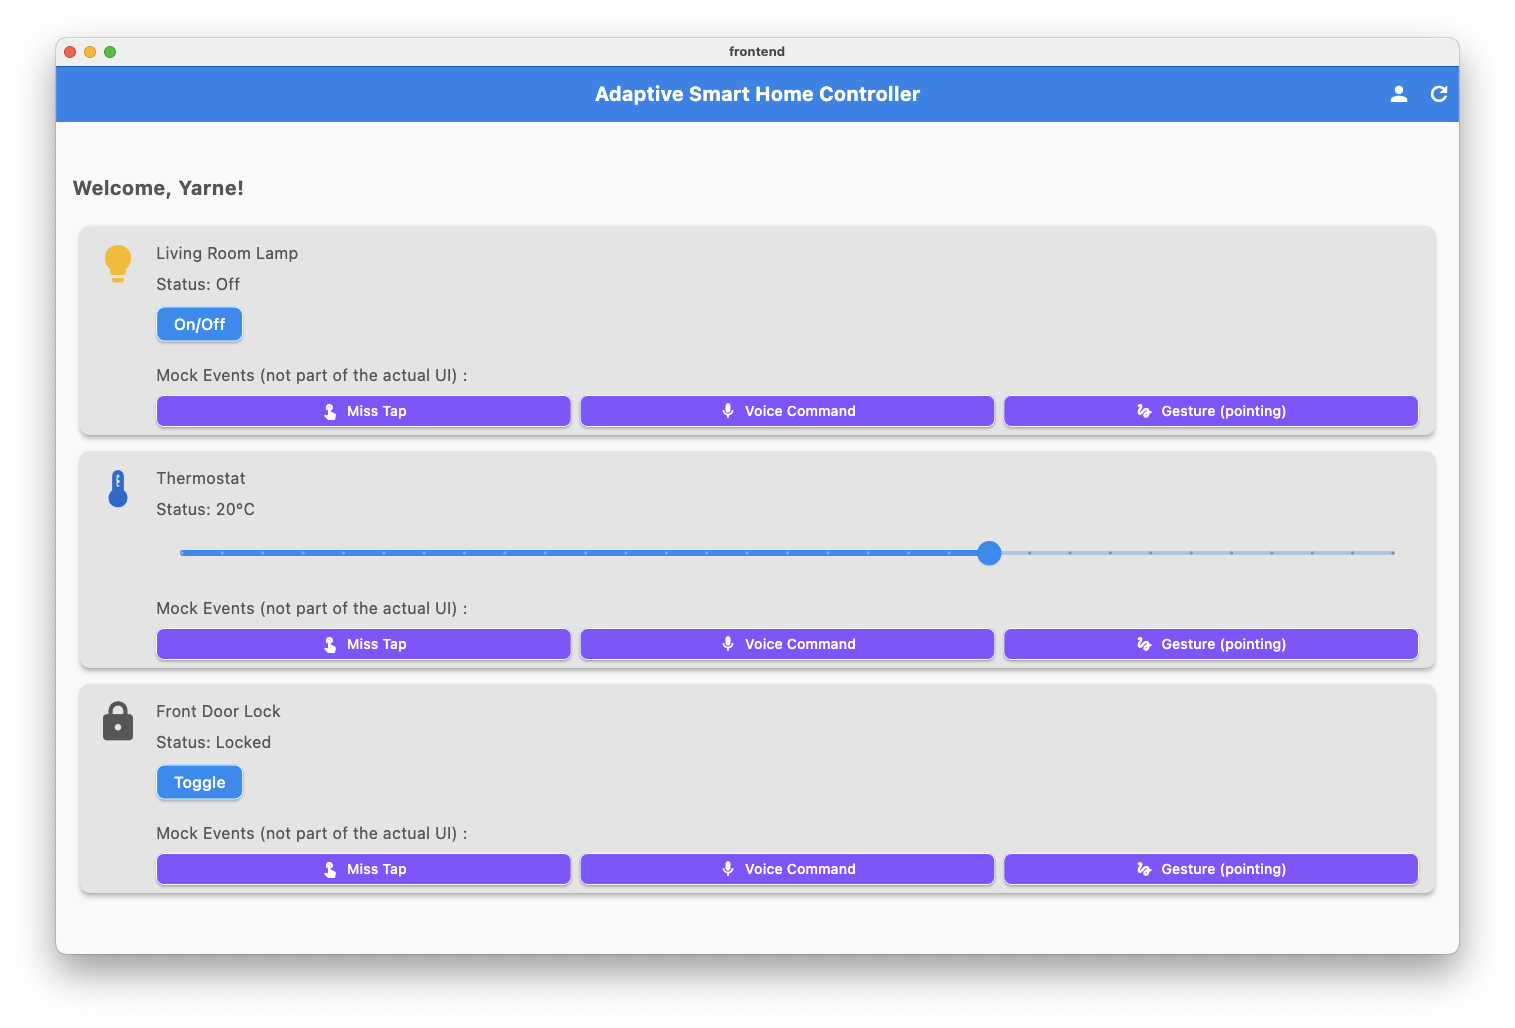
\includegraphics[width=\linewidth]{images/fig_ui_overview.png}
    \caption*{Before: standard interface with small targets}
\end{minipage}\hfill
\begin{minipage}{.5\linewidth}
    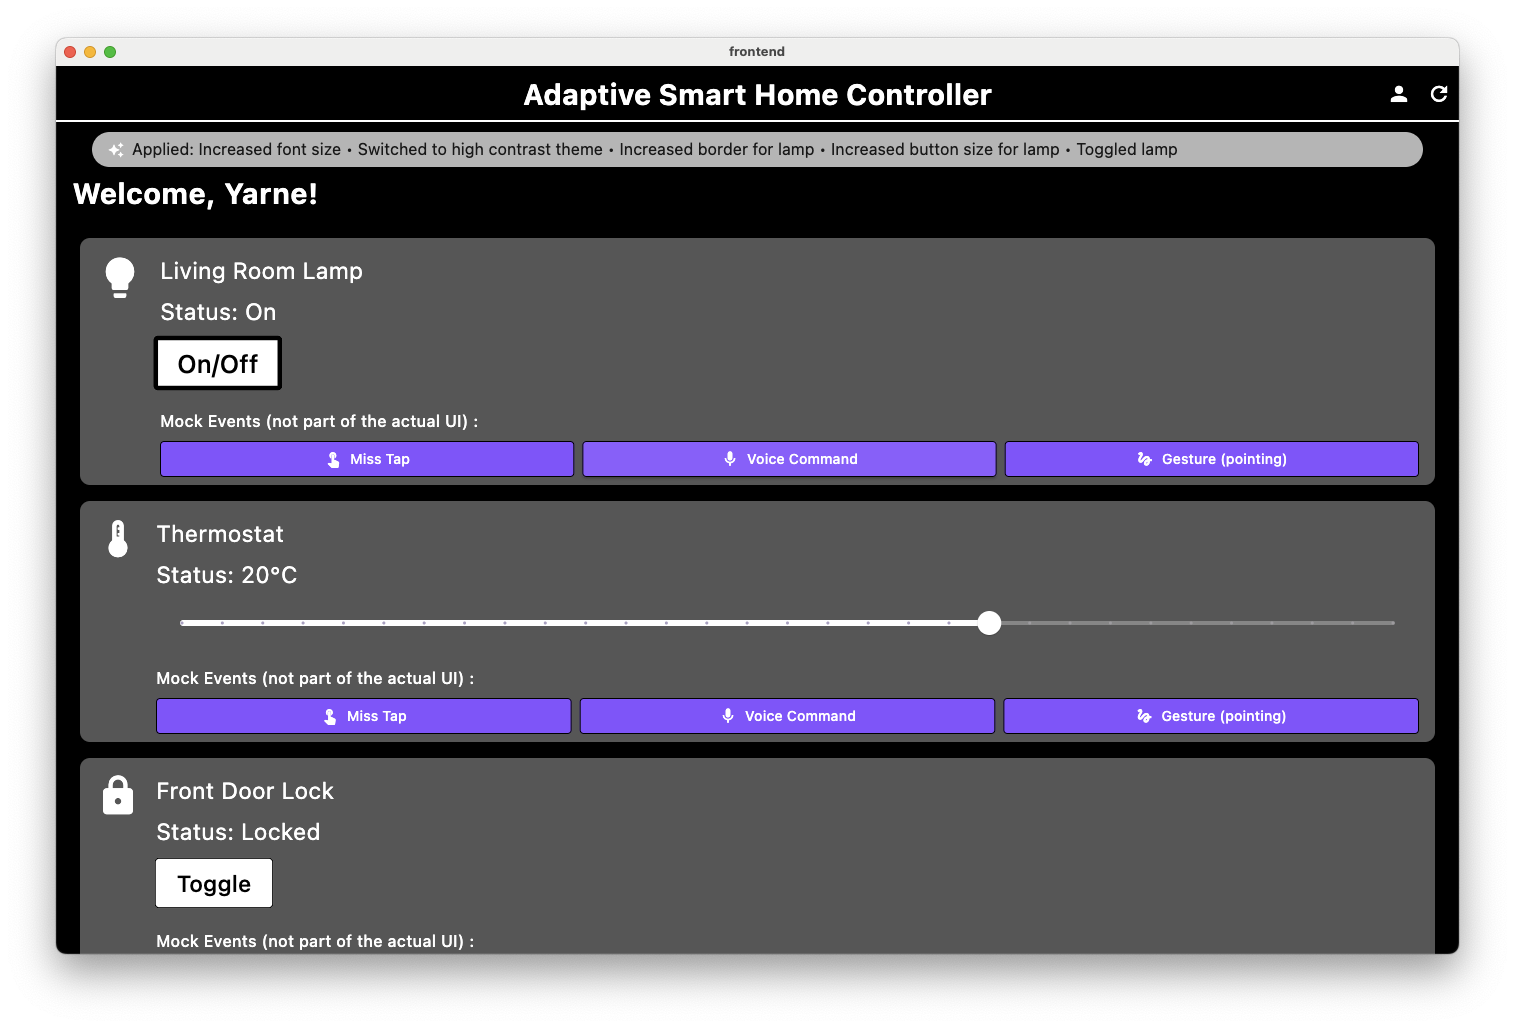
\includegraphics[width=\linewidth]{images/fig_adapt_after.png}
    \caption*{After: enlarged targets, enhanced contrast, stronger borders}
\end{minipage}
\caption{Real-time adaptation applied after miss-tap event for visually impaired user.}
\label{fig:before-after-adaptation}
\end{figure}

\section{Backend Injection Interface}

\subsection{Purpose and Scope}
This lightweight Flutter tool exposes a direct interface to the SIF backend for debugging and evaluation. It lets a researcher inject or edit \emph{profiles} and \emph{events}, send them to the backend over WebSocket/HTTP, and immediately inspect the returned \texttt{\{adaptations:[...]\}} along with the server-side interaction history per user. It is separate from the end-user UI and optimized for fast iteration. 

\subsection{Architecture and Data Flow}
On launch the app opens a WebSocket to \texttt{ws://localhost:8000/ws/adapt} and listens for JSON replies containing an \texttt{adaptations} array. Profile updates are sent via HTTP \texttt{POST /profile}, while the history panel pulls entries from \texttt{GET /full\_history}. Incoming WS frames are decoded and the \texttt{adaptations} list is rendered; after each reply the tool refreshes history via HTTP to keep the view in sync. 

\subsection{Controls: Profiles and Events}
The left column edits the \emph{profile} (free-form JSON or prefilled “Motor Impaired” / “Hands-Free”), visualizing key blocks like \texttt{accessibility\_needs} and \texttt{input\_preferences}. The right column edits the \emph{event} (free-form JSON or predefined “Miss-Tap on Play”, “Voice Play Command”, “Gesture Point”). Both editors pretty-print JSON and show an iconized summary (user, modality, target). This enables fast A/B of context vs. input without leaving the app (see figure \ref{fig:backend-inject-adapt-config} for an example).

\begin{figure}[h]
\centering
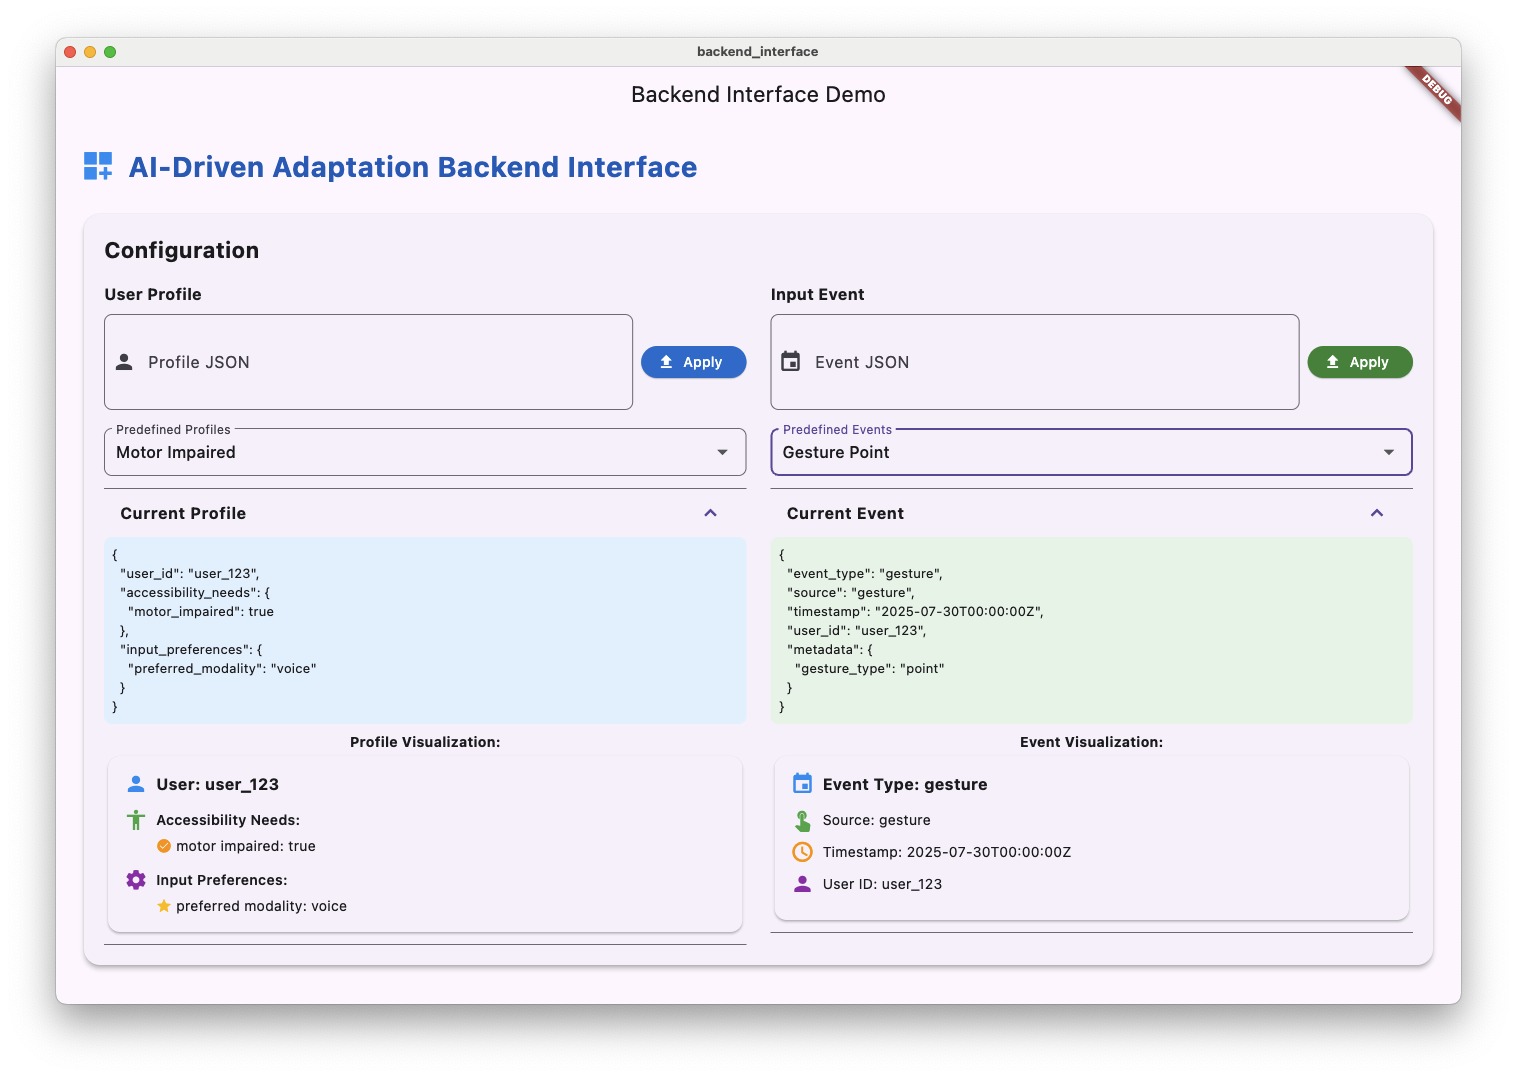
\includegraphics[width=.5\linewidth]{images/fig_backend_inject_config.png}\hfill
\caption{Backend Injection Interface: configuration and live JSON visualization.}
\label{fig:backend-inject-adapt-config}
\end{figure}

\subsection{Adaptation Response View}
Pressing \emph{Get Suggestions} sends the current event (after posting the profile), shows a spinner, then lists each adaptation with an action-specific icon and a compact, human-readable summary (e.g., “Switch to voice mode” or “Increase contrast”). The mapping covers common actions such as \texttt{switch\_mode}, \texttt{increase\_contrast}, \texttt{trigger\_button}, \texttt{simplify\_layout}, and geometry actions. Unknown actions fall back to a generic renderer, keeping the tool resilient to backend experiments (see figure \ref{fig:backend-inject-adapt} for an example). 

\begin{figure}[h]
\centering
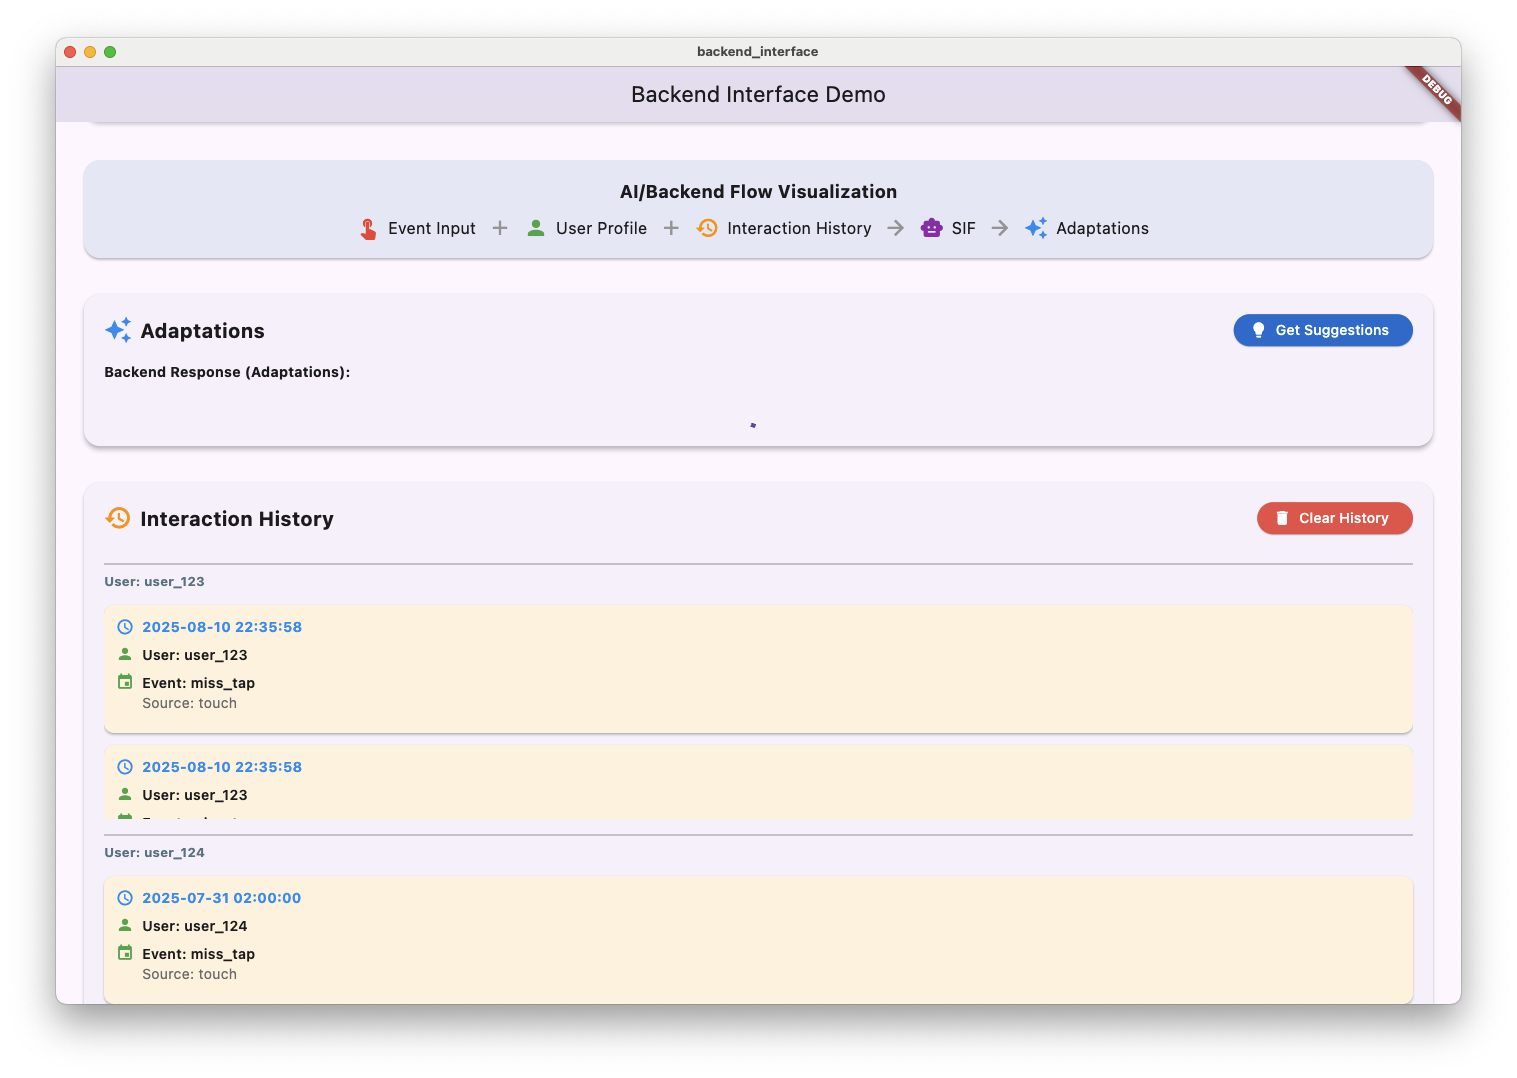
\includegraphics[width=.5\linewidth]{images/fig_backend_inject_adapt_before.png}\hfill
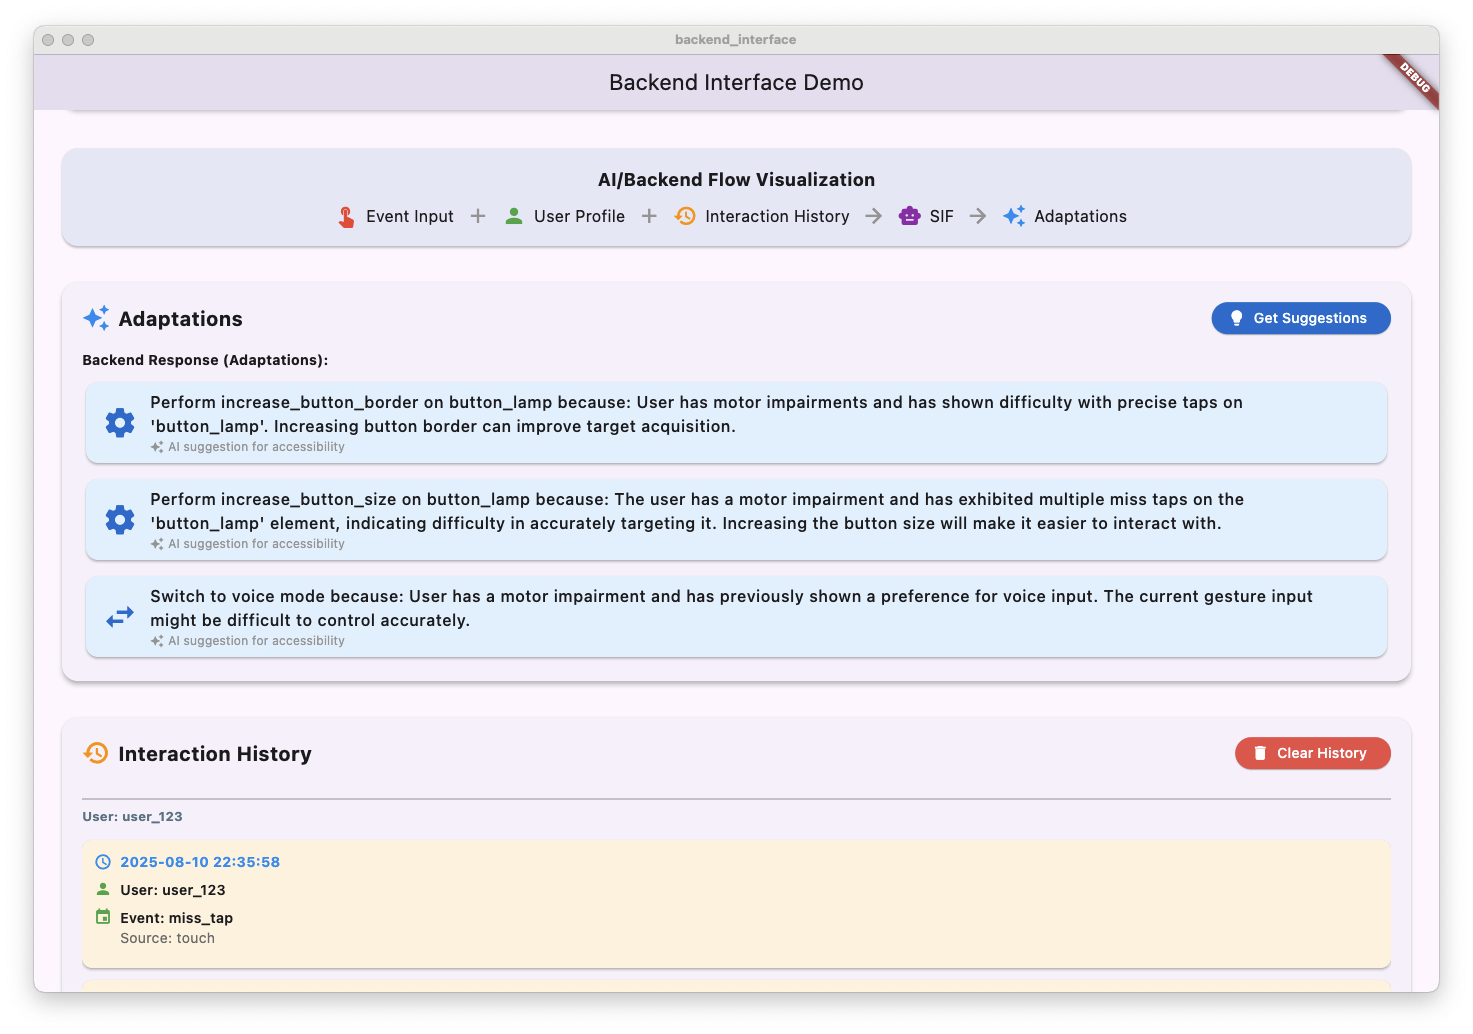
\includegraphics[width=.5\linewidth]{images/fig_backend_inject_adapt_after.png}
\caption{Example adaptation list before/after a pointing gesture event.}
\label{fig:backend-inject-adapt}
\end{figure}

\subsection{Interaction History Panel}
The bottom card fetches \texttt{history} from the backend and renders each entry (timestamp, user, event type/source) plus the associated adaptations. This provides a quick audit trail to verify that profile changes affect subsequent suggestions and to spot repeated error patterns (e.g., consecutive miss-taps). A “Clear History” button resets the local view; history retrieval is refreshed after each WS reply to keep causality visible.

\subsection{Operational Notes and Limitations}
The app assumes a running backend at \texttt{localhost:8000}. Profile JSON is posted verbatim; there is no schema validation beyond backend checks. The WS channel is established once on init; a commented reconnection helper is included for future hardening. Timeouts and transport errors are surfaced minimally to keep the UI uncluttered. This is created as a developer tool and is not intended for end-users.

\section{Cross-Platform SwiftUI Example}

\subsection{Purpose and Scope}
This minimal SwiftUI app demonstrates that a thin, platform-native adapter plus a small view layer are sufficient to integrate with the SIF backend. It mirrors the Flutter contract: create (or fetch) a user profile over HTTP, stream events over WebSocket, and apply the returned \texttt{\{adaptations:[...]\}} envelope to the UI state. The example targets iOS/macOS (Swift~5.7+, iOS~15+) and may require ATS exceptions for local HTTP/WS during development.

\subsection{Adapter and Transport}
The \texttt{AdaptiveUIAdapter} is an \texttt{ObservableObject} that (i) ensures the profile exists via \texttt{GET /profile/
\{user\_id\}} and \texttt{POST /profile}, (ii) opens a \texttt{URLSessionWebSocketTask} to \texttt{/ws/adapt}, and (iii) exposes \texttt{sendEvent(\,)} and an \texttt{onAdaptations} callback for the UI. Incoming frames are decoded from a wrapped
 \texttt{Envelope\{adaptations:[...]\}} into an array of \texttt{Adaptation}. On receive errors it reconnects after a short delay, keeping the session resilient for local testing and debugging. Events are encoded with \texttt{JSONEncoder.convertToSnakeCase}, matching the backend’s snake\_case contract.

\subsection{Minimal UI and State Mapping}
\texttt{AdaptiveUIApp} wires the adapter into the environment and renders a single \texttt{ContentView} that shows a lamp card, a few “send event” buttons, and a live list of the most recent adaptations (see figure \ref{fig:swift-adapt} for a before-after example). The view holds a small set of reactive states \texttt{buttonScale}, \texttt{borderWidth}, \texttt{highContrast}, \texttt{fontScale}, \texttt{spacing}, and \texttt{tooltip}, that the \texttt{apply(\,)} function updates based on \texttt{action}/\texttt{target}/\texttt{value}/\texttt{mode}. Concretely:  
\emph{increase\_button\_size} multiplies \texttt{buttonScale}, \emph{increase\_font\_size} scales text, \emph{increase\_contrast} toggles a high-contrast color scheme, \emph{increase\_button\_border} sets a visible outline, \emph{adjust\_spacing} scales inter-control spacing (clamped), \emph{show\_tooltip} surfaces the model’s reason string, and \emph{trigger\_button} toggles the lamp state. This mirrors the Flutter mapping but proves the contract is UI-framework agnostic. 

\subsection{Event Injection}
Three buttons generate representative events: a miss-tap (\texttt{event\_type="miss\_tap"} with coordinates), a simple voice command (\texttt{event\_type="voice"} with \texttt{metadata.command}), and a local tap. The miss-tap and voice paths serialize to JSON and are sent over WS; the tap path is stubbed to flip local state, emphasizing that production UIs would simply send the tap event the same way. 

\subsection{Usage and Limitations}
On launch, the adapter creates a minimal default profile when needed, connects WS, and begins listening. Pressing “Miss-tap” or “Voice” triggers a backend roundtrip; the adaptation list below the card updates immediately and \texttt{apply(\,)} mutates view state. The demo intentionally omits persistence and complex navigation; its goal is to show that the SIF contract (profile endpoints, WS envelope, action names) can be integrated cleanly into SwiftUI with \(\approx\)~a hundred lines of adapter+view code.

\begin{figure}[h]
\centering
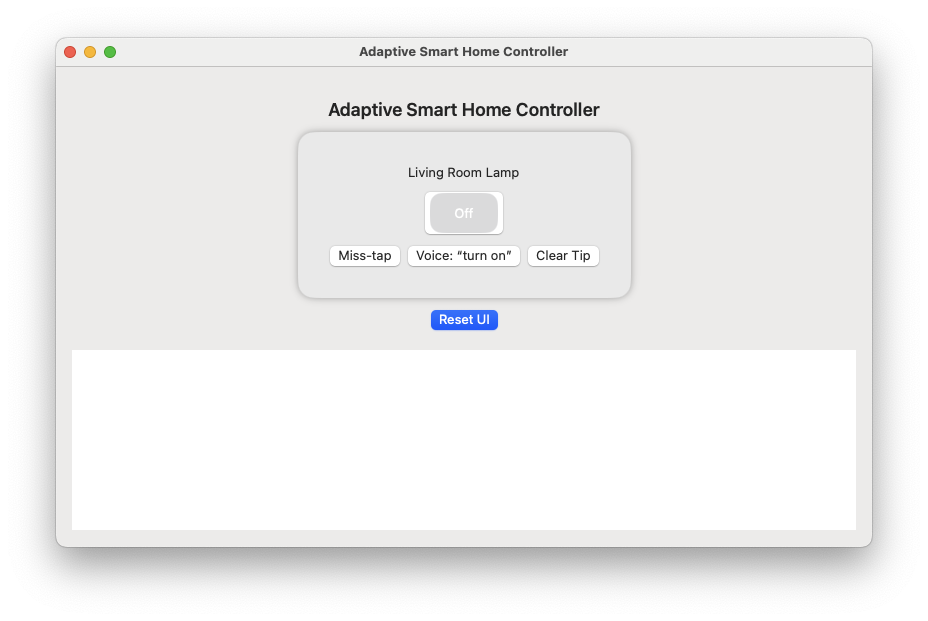
\includegraphics[width=.5\linewidth]{images/fig_swift_before.png}\hfill
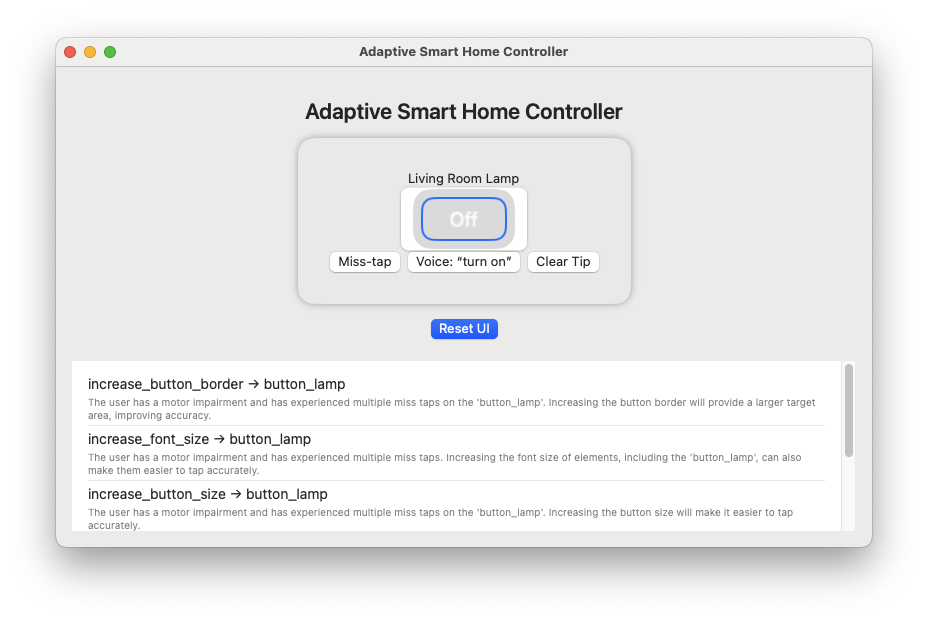
\includegraphics[width=.5\linewidth]{images/fig_swift_after.png}
\caption{Example SwiftUI app before/after a miss\_tap event.}
\label{fig:swift-adapt}
\end{figure}

\section{Design Decisions}
The design of the Adaptive Multimodal GUI Framework using LLMs reflects a series of deliberate choices aimed at balancing accessibility, performance, scalability, extensibility, and ease of integration. These decisions were made with the primary goal of delivering real-time, personalised adaptations for motor-impaired, visually impaired, and hands-free users, while ensuring that the framework remains modular and adaptable to future platforms and domains.

\subsection{Modularity Over Monolithic Design}
\textbf{Decision:} The framework adopts a modular three-layer architecture (Frontend, Input Adapter, SIF Backend) with clear separation of concerns, connected through a standardised JSON contract.

\textbf{Reasoning:}
\begin{itemize}
    \item \textbf{Flexibility:} Each layer can be updated or replaced independently, enabling deployment across different platforms such as Flutter, SwiftUI, or future platforms without reworking the entire system.
    \item \textbf{Extensibility:} The JSON contract in the Input Adapter Layer allows new modalities (e.g., eye tracking) to be integrated without modifying backend logic.
    \item \textbf{Developer accessibility:} Modularity simplifies integration, requiring minimal code for event handling and adaptation application.
\end{itemize}

\subsection{WebSocket for Real-Time vs. HTTP for Batch Processing}
\textbf{Decision:} The framework uses WebSocket (\texttt{/ws/adapt}) for real-time event processing and adaptation delivery, with HTTP (\texttt{/full\_history, /profile}) for debugging, developer tooling and profile management.

\textbf{Reasoning:}
\begin{itemize}
    \item \textbf{Low Latency:} WebSocket enables fast and bidirectional sending of data like adaptations (e.g., scaling a button after a miss-tap).
    \item \textbf{Reliability:} HTTP supports robust profile updates (\texttt{POST} \texttt{/profile}), ideal for non-real-time scenarios or debugging.
    \item \textbf{Accessibility:} Real-time feedback enhances usability for motor-impaired or hands-free users, where delays could disrupt interaction. 
\end{itemize}

\subsection{MongoDB for Persistent Storage}
\textbf{Decision:} MongoDB is used for storing user profiles, interaction history, and adaptation logs, with \texttt{user\_id} indexing and capped history arrays (10 events).

\textbf{Reasoning:}
\begin{itemize}
  \item \textbf{Scalability:} MongoDB’s NoSQL design and indexing ensure fast queries for large user bases, critical for real-world deployment.
  \item \textbf{Flexibility:} JSON-like documents align with the framework’s JSON contract, simplifying profile/history storage.
  \item \textbf{Continuous Learning:} Retaining a limited history supports adaptive behaviour, such as making permanent size adjustments after repeated miss-taps.
\end{itemize}

\subsection{Rule-Based Fallback with LLM Reasoning}
\textbf{Decision:} SIF combines rule-based logic (e.g., \texttt{if miss\_tap then increase\_size}) with LLM reasoning for creative adaptations, with rules as a fallback for LLM failures or time-outs, since LLM's can have high respond latencies.

\textbf{Reasoning:}
\begin{itemize}
  \item \textbf{Reliability:} Rules ensure deterministic adaptations (e.g., button enlargement for miss-taps) when LLM responses are unavailable or hallucinate.
  \item \textbf{Novelty:} LLM enables context-aware, proactive suggestions (e.g., \verb|switch_mode: voice| for hands-free users), advancing beyond static rules.
  \item \textbf{Accessibility:} Hybrid approach ensures consistent support for motor-impaired, visually impaired users (e.g., high-contrast text).
\end{itemize}

\subsection{Multi-agent LLM reasoning (MA-SIF) vs single-agent LLM reasoning (normal SIF)}
A key architectural decision in the framework is the adoption of multi-agent LLM reasoning (MA-SIF) over a single agent LLM approach (normal SIF). In the single agent SIF model, one LLM is responsible for interpreting all input events and generating adaptation actions. While this simplifies integration and reduces system complexity, it can limit the granularity and specialization of adaptation logic, especially as the diversity of user needs and input modalities grows.

MA-SIF, by contrast, distributes reasoning across multiple specialized LLM agents, each focused on a distinct domain such as UI adaptations, geometry/layout changes, input modality management, and validation. This separation of concerns enables each agent to leverage tailored prompts, domain-specific knowledge, and focused reasoning strategies, resulting in more nuanced and context-aware adaptation suggestions. The validator agent further ensures that outputs from other agents are coherent, non-conflicting, and accessibility-compliant.

The multi-agent approach offers several advantages: \begin{itemize} \item \textbf{Scalability:} New agents can be added to address emerging modalities or adaptation domains without disrupting existing logic. \item \textbf{Extensibility:} Prompts and allowed actions can be updated independently for each agent, supporting rapid iteration and domain-specific improvements. \item \textbf{Robustness:} Specialized agents reduce the risk of LLM hallucinations or conflicting adaptations, as validation is enforced before application. \item \textbf{Personalization:} Agents can incorporate user profiles and history more effectively, enabling targeted adaptations for motor-impaired, visually impaired, or hands-free users. \end{itemize}

\section{Implementation Challenges and Solutions}
Developing the Adaptive Smart Home Controller exposed several practical challenges, ranging from LLM-specific issues to general real-time system concerns. These were addressed through a mix of architectural decisions, fallback mechanisms, and compromises designed to keep the prototype functional and reliable under varying conditions.

\subsection{LLM reliability and output consistency}
One of the most persistent challenges was ensuring that the multi-agent LLM pipeline returned valid, schema-compliant output. Despite strict prompts and an explicit allowed-actions list, hallucinations still occurred, producing unsupported actions, targeting non-existent elements, or returning unreasonable values such as excessively large scaling factors. These errors risked breaking the layout or producing jarring visual changes. To mitigate this as described earlier, a validator agent was introduced to consolidate and correct suggestions before they reached the frontend. However, this validation step added extra latency and still could not guarantee complete protection against invalid values, making additional frontend-side checks a sensible next step for future versions.

\subsection{Performance under real-time constraints}
Adaptation latency was a critical factor for usability, particularly in accessibility scenarios where delayed feedback can reduce trust in the system. Smaller LLM models were assigned to the suggestion agents to keep their execution time within fractions of a second, while the validator, which required more context and reasoning, used a larger model with a higher timeout budget. Even so, occasional slowdowns occurred due to network latency or provider-side delays. The backend was therefore designed to apply partial results if all agents did not respond in time, ensuring that at least some adaptations reached the user quickly.

\subsection{Safeguards against malicious or replay attacks}
In its current form, the system does not include strong safeguards against replay attacks or intentionally crafted events designed to trigger disruptive adaptations. This is acceptable in a controlled research environment but would require strict validation and authentication for production deployment. Measures such as signing WebSocket messages, verifying sequence numbers, and rejecting stale or malformed events would be necessary to prevent exploitation as well as extra protections in the adapter or frontend. Furthermore is \texttt{user\_id} hijacking, where an attacker submits events under a different user’s profile possible, since no \texttt{user\_id} checks are done on returning adaptations. Future mitigations such as implementing \texttt{user\_id} verification and event signing will be necessary to address these vulnerabilities. This was intentional for the scope and development time constraints of this research.

\subsection{Testing with incomplete modalities}
Live gesture tracking and voice inputs were not integrated in this iteration, which meant that related adaptations had to be tested using simulated events. While this allowed the adaptation logic to be validated end-to-end, it did not account for the noise, recognition errors, or latency introduced by real input devices. Future work will need to focus on replacing these simulated events with actual input sources to fully evaluate performance in realistic conditions.

\subsection{Security and trust boundaries}
In its current implementation state, the backend accepts connections from any origin and does not require authentication for profile creation or event submission. Currently a pure localhost setup is implemented for the entire backend. This was a deliberate decision to speed up testing across platforms, but would need to be replaced with stricter CORS rules, token-based authentication, and access control in production. Without these measures, the system is vulnerable to unsolicited adaptation requests from external sources. Furthermore, some config files such as \texttt{sif\_config.json} do not have the necessary validation checks in the backend, while the validator agent is necessary, nothing stops it from being removed.

\section{Chapter Summary}
This chapter has detailed the implementation of the Adaptive Smart Home Controller as the primary proof-of-concept for the multimodal AI-driven GUI framework. The system was realised as a three-layer architecture, consisting of a Flutter-based frontend for rendering and applying adaptations, an Input Adapter Layer for standardising and transmitting events, and a FastAPI-based backend implementing multi-agent Smart Intent Fusion with MongoDB for persistent profile and history storage.

Key implementation aspects included the construction of a dynamic adaptation pipeline capable of applying size, contrast, modality, and content changes in real time, and the use of a strict JSON schema to maintain consistency between layers. While some modalities such as voice and gesture inputs were simulated for demonstration purposes, the system was designed so that integrating real devices will require minimal architectural changes.

The prototype also faced practical challenges, including LLM output validation, latency management, security considerations, and the absence of certain safeguards against malicious or replayed events. These were addressed through a combination of a validator agent, conservative rule-based fallbacks, partial-result handling, and a modular design that isolates critical components.

In its current state, the implementation demonstrates that the framework can deliver personalised, accessibility-focused adaptations in a responsive and modular manner, even under the constraints of a prototype environment. The next chapter evaluates this implementation through a feasibility study, assessing its responsiveness, adaptability, and practical potential in simulated real-world scenarios.

%Chapter 6
\chapter{Evaluation}
\label{ch:evaluation}

\section{Evaluation Overview}
The goal of evaluating the implementation is by feasibility study, to check whether the multimodal AI-driven adaptation pipeline works end-to-end under realistic interaction traces, and whether it does so in a way that is useful for accessibility. Concretely:
\begin{enumerate}
    \item \textbf{Adaptation validity:} Does the backend return schema-valid adaptation objects across different user profiles and modalities?
    \item \textbf{Accessibility relevance:} Do the proposed adaptations match the user’s needs (motor, visual, hands-free) and the observed errors (e.g., miss-taps, slider overshoot)?
    \item \textbf{Latency:} What is the end-to-end response time (p50/p90/max) under the chosen backend configuration?
\end{enumerate}

\section{Methodology}
\paragraph{Profiles and Runs:}
Six user profiles (P0--P5) were used to cover a range of interaction needs, including neutral, motor-impaired, visual-impaired, and hands-free preferences, including combined needs:
\begin{itemize}
    \item \textbf{P0 (Baseline):} No specific accessibility needs.
    \item \textbf{P1 (Motor-impaired):} Requires larger touch targets; keyboard preferred navigation.
    \item \textbf{P2 (Visual-impaired):} Needs adaptations for visual impairment (e.g., larger font).
    \item \textbf{P3 (Hands-free):} Prefers voice control and hands-free interactions.
    \item \textbf{P4 (Combined):} Needs adaptations for both motor and hands-free interactions (voice preferred).
    \item \textbf{P5 (Combined):} Needs adaptations for motor and visual impairments (voice preferred).
\end{itemize}
For each of the six profiles, two runs were executed to allow a small interaction history to build up over time. Each run consisted of the same 7-event sequence (14 events per profile, 84 events total). See Table~\ref{tab:user-profile-mapping} for the user profile mapping.

\begin{table}[h]
\centering
\caption{User profile mapping for evaluation runs}
\begin{tabular}{ll}
\toprule
\textbf{Profile} & \textbf{Declared Needs} \\
\midrule
P0 & Baseline (no declared needs) \\
P1 & Motor-impaired, keyboard preferred \\
P2 & Visual-impaired, larger font \\
P3 & Hands-free preferred, voice modality \\
P4 & Motor-impaired + hands-free, voice modality \\
P5 & Visual-impaired + motor-impaired, voice modality \\
\bottomrule
\end{tabular}
\label{tab:user-profile-mapping}
\end{table}

\paragraph{Event Suite:}
The event suite mixes errors and successful attempts across modalities and targets (smart-home “lamp”, “thermostat”, “lock”):
\begin{itemize}
    \item \texttt{miss\_tap} on buttons (lamp/lock)
    \item \texttt{voice} commands (turn\_on/unlock/adjust)
    \item \texttt{gesture} inputs (point at lamp)
    \item \texttt{slider\_miss} with overshoot (thermostat)
\end{itemize}
This combination intentionally triggers common accessibility challenges (tap precision, slider control, and mode switching between touch/voice/gesture).

\paragraph{Backend Configuration and Metrics:} 
All traces were evaluated using the MA-SIF (balanced) configuration (Table~\ref{tab:ma-sif-config}), with each event’s adaptation response checked for schema validity. For every event, the classification path (validator vs. fallback) and latency metrics (p50/p90/max) were recorded. Analysis was performed using the project’s extraction and evaluation scripts, which flatten the JSONL logs to CSV, compute summary statistics, and export figures and tables for reporting.
\begin{table}[htb]
\centering
\caption{MA-SIF (balanced) agent configuration}
\label{tab:ma-sif-config}
\begin{tabular}{lcccc}
\toprule
\textbf{Agent} & \textbf{Model} & \textbf{Thinking Budget} & \textbf{Temperature} & \textbf{Timeout (s)} \\
\midrule
UI         & gemini-flash-lite & 0   & 0.2 & 15 \\
Geometry   & gemini-flash-lite & 0   & 0.2 & 15 \\
Input      & gemini-flash-lite & 0   & 0.2 & 15 \\
Validator  & gemini-flash      & -1  & 0.3 & 30 \\
\bottomrule
\end{tabular}
\label{tab:ma-sif-config-eval}
\end{table}

\paragraph{Operational definitions (micro-clarifications):}
\textbf{Schema-valid} means the response object conforms to the adaptation JSON schema (valid action names, allowed parameter ranges, resolvable UI targets, and consistency checks enforced by the Validator). 
\textbf{Latency} is measured client-side per event as $\Delta t = t_{\text{recv}} - t_{\text{send}}$, covering multi-agent coordination and Validator checks.

\section{System Demonstration and Experimental Setup}
\paragraph{Evaluation Scenarios:}
The Adaptive Smart Home Controller using LLMs was evaluated by executing the 7-event sequence with 2 runs on each profile. Typical flows included:
\begin{itemize}
    \item A user misses a tap on the lamp button $\rightarrow$ the system proposes larger buttons/borders and optionally switches to voice input.
    \item The thermostat slider overshoots $\rightarrow$ the system proposes a larger slider and spacing adjustments.
    \item A voice command is issued (turn on lamp / unlock door) $\rightarrow$ the system either confirms voice as the preferred mode or combines it with gesture hints.
\end{itemize}

\paragraph{Hardware and Environment:}
All experiments in this thesis were executed on a single development machine in a controlled home environment (none to low network contention). Latency is end-to-end from event send to response received on the client.
Hardware configuration:
\begin{itemize}
    \item \textbf{Hardware:} MacBook Pro, M1 Max CPU, 32\,GB RAM, 32-core GPU
    \item \textbf{Software:} macOS 15.6 (Sequoia), Python 3.9+
    \item \textbf{Environment:} Localhost, no external API calls
\end{itemize}
\newpage
\section{Results and Observations}
\subsection{Overall Summary}
Across 84 events and 6 user profiles, the system produced adaptations with: (Table~\ref{tab:overall-feasibility})
\begin{itemize}
    \item \textbf{Schema-valid outputs:} 84.52\% of events.
    \item \textbf{Classification path:} 100\% processed via the Validator (no fallback used).
    \item \textbf{Latency:} p50 13.19 s, p90 17.13 s, max 21.10 s.
\end{itemize}

\begin{table}[htb]
  \centering
  \caption{Overall feasibility results with MA-SIF (balanced).}
  \begin{tabular}{lr}
    \toprule
    \textbf{Metric} & \textbf{Value} \\
    \midrule
    Events (total) & 84 \\
    Users (total) & 6 \\
    Schema-valid outputs (\%) & 84.52 \\
    Validated by Validator (\%) & 100.00 \\
    Latency $p_{50}$ (s) & 13.19 \\
    Latency $p_{90}$ (s) & 17.13 \\
    Latency max (s) & 21.10 \\
    \bottomrule
  \end{tabular}
  \label{tab:overall-feasibility}
\end{table}

The most frequent actions were:
\begin{itemize}
    \item \texttt{switch\_mode} (87): often recommending voice mode.
    \item \texttt{increase\_button\_size} (74), \texttt{increase\_button\_border} (69), \texttt{increase\_font\_size} (66).
    \item \texttt{increase\_slider\_size} (28), \texttt{increase\_contrast} (19).
    \item Less frequent: \texttt{trigger\_button} (9), \texttt{adjust\_spacing} (9).
\end{itemize}
Because multiple suggestions can be attached to one event, action counts exceed the number of events. Top targets were the lamp, thermostat, and lock, with miss-taps most often on lamp and lock (by design).

\paragraph{Interpretation:} The system strongly prioritizes motor-related support (larger targets, borders, spacing) and modal switching to voice when it detects tap/slider errors, exactly the pattern that is needed for motor-impaired and hands-free users. Vision-related support (font size and contrast) also appears consistently, but is less prominent than motor support in this trace.

\subsection{Per-Profile Outcomes}
Per-profile schema validity and latency (median p50, higher-tail p90, and worst-case max): (Table~\ref{tab:per-profile})
\begin{itemize}
    \item \textbf{P0 (baseline)}: 78.57\% valid; $p50 \approx 16.02\,\mathrm{s}$; $p90 \approx 20.23\,\mathrm{s}$; max $21.10\,\mathrm{s}$.
    \item \textbf{P1 (motor)}: 85.71\% valid; $p50 \approx 13.19\,\mathrm{s}$; $p90 \approx 16.78\,\mathrm{s}$; max $17.43\,\mathrm{s}$.
    \item \textbf{P2 (visual)}: 85.71\% valid; $p50 \approx 13.65\,\mathrm{s}$; $p90 \approx 16.46\,\mathrm{s}$; max $19.04\,\mathrm{s}$.
    \item \textbf{P3 (hands-free)}: 71.43\% valid; $p50 \approx 11.82\,\mathrm{s}$; $p90 \approx 14.68\,\mathrm{s}$; max $16.49\,\mathrm{s}$.
    \item \textbf{P4 (motor + hands-free)}: 85.71\% valid; $p50 \approx 13.63\,\mathrm{s}$; $p90 \approx 15.76\,\mathrm{s}$; max $17.91\,\mathrm{s}$.
    \item \textbf{P5 (visual + motor)}: 100.00\% valid; $p50 \approx 12.70\,\mathrm{s}$; $p90 \approx 16.25\,\mathrm{s}$; max $16.60\,\mathrm{s}$.
\end{itemize}

\begin{table}[htb]
  \centering
  \caption{Per-profile schema validity and latency under MA-SIF (balanced).}
  \begin{tabular}{l l r r r r}
    \toprule
    \textbf{Profile} & \textbf{Declared needs} & \textbf{Valid (\%)} & \textbf{$p_{50}$ (s)} & \textbf{$p_{90}$ (s)} & \textbf{max (s)} \\
    \midrule
    P0 & Baseline & 78.57 & 16.02 & 20.23 & 21.10 \\
    P1 & Motor & 85.71 & 13.19 & 16.78 & 17.43 \\
    P2 & Visual & 85.71 & 13.65 & 16.46 & 19.04 \\
    P3 & Hands-free & 71.43 & 11.82 & 14.68 & 16.49 \\
    P4 & Motor + Hands-free & 85.71 & 13.63 & 15.76 & 17.91 \\
    P5 & Visual + Motor & 100.00 & 12.70 & 16.25 & 16.60 \\
    \bottomrule
  \end{tabular}
    \label{tab:per-profile}
\end{table}
\newpage
\paragraph{Observations:}
\begin{itemize}
    \item Highest validity appears for combined needs (P5), likely because the event suite provides strong, consistent signals (miss-taps + slider overshoot) that align with the rules and model prior for motor/visual support.
    \item Lowest validity is P3 (hands-free) at 71.43\%. Even though P3 shows the best latency, hands-free preference alone may result in fewer structural UI changes (e.g., fewer size/contrast edits), and the Validator may reject marginal suggestions more often. This indicates room to enrich the hands-free policy (e.g., more explicit voice/gesture affordances and confirmation prompts).
    \item Latency is in the 11.8--16.0 s p50 band across profiles under the MA-SIF (balanced) config. The spread between p50 and p90 ($\approx 3$--$4\,\mathrm{s}$) suggests predictable tail behavior, with a single global max near 21 s.
\end{itemize}

\subsection{Accessibility Impact Analysis}
The distribution of suggested actions aligns with both the declared needs of the profiles and the error patterns in the event suite:

\begin{itemize}
  \item \textbf{Motor support (P1, P4, P5).} Frequent enlargement of buttons and sliders, thicker borders, and increased spacing; when repeated miss-taps occur, the policy often proposes \texttt{switch\_mode} to voice to reduce precision demands.
  \item \textbf{Visual support (P2, P5).} Font-size increases appear consistently; contrast boosts are present but less frequent, which is expected given the suite skews toward motor-related errors (miss-taps, slider overshoot).
  \item \textbf{Hands-free (P3, P4).} Many \texttt{switch\_mode} $\rightarrow$ voice suggestions; adding explicit voice-first affordances (prompting, feedback, focus outlines) is a promising next step to raise acceptance.
\end{itemize}

Overall, the system responds not only to immediate problems during interaction, such as missed taps or slider overshoots, but also to the user’s stated preferences, such as wanting to use voice commands. This means the system can react to fix recent mistakes while also making changes in advance to support the way a user prefers to interact.

In practice, this results in a strong focus on motor support, such as making buttons and sliders bigger and adding thicker borders or more space. Visual support appears where needed, such as increasing text size and contrast. For hands free users, the system often switches to voice control to reduce the need for precise touch. The share of actions aimed at each of these accessibility categories is shown in following Table~\ref{tab:overall-accessible-share}, divided into motor, visual, and hands free support.

\begin{table}[htb]
\centering
\caption{Overall accessibility-targeted actions from the global action distribution. Categories: motor, visual, hands-free.}
\label{tab:overall-accessible-share}
\begin{tabular}{l r}
\toprule
\textbf{Metric} & \textbf{Value} \\
\midrule
Total actions (overall) & 361 \\
Accessibility-targeted (motor/visual/hands-free) & 352 \\
Share accessibility-targeted (\%) & 97.51 \\
\midrule
Aggregate aligned \% across profiles (excluding P0)\textsuperscript{*} & 63.72 \\
\bottomrule
\end{tabular}

\smallskip
\raggedright \textsuperscript{*}Computed from each profile's top-5 actions only; may underestimate alignment if lower-frequency actions are omitted.
\end{table}

\subsection{Adaptation Performance (Latency)}
With \textbf{MA-SIF (balanced)}, median latency sits around 13 s overall (p50 13.19 s / p90 17.13 s / max 21.10 s). For a first feasibility pass with multiple agents and validation, this is acceptable for asynchronous UI adaptation (e.g., adapting after an error or between interactions). For strict real-time use (e.g., continuous VR hand-tracking), optimizations are needed (Section~6.6).

\section{Discussion of Results}
\paragraph{What worked:}
The pipeline produced valid, targeted adaptations in most cases (84.5\% valid overall, 100\% through the Validator path). The action distribution shows the system prioritizes the right things for accessibility (larger targets, borders, contrast/font, and mode switching). This is consistent with the global action mix, where the majority of suggestions are accessibility-focused rather than generic UI operations.

\paragraph{What needs work:}
Hands-free profiles (P3) had lower validity, likely because they trigger fewer structural UI changes while the Validator rejects marginal or redundant mode suggestions. The plan is to surface explicit voice UI hints, add confirmation steps, and investigate voice-first layouts to improve acceptance. In addition, the share of \emph{profile-aligned} actions should be raised by weighting suggestions more strongly toward the user’s declared needs, not only toward recent errors.

\paragraph{Why latency looks like this:}
The balanced multi-agent + Validator path introduces coordination and checking overhead. This is the trade-off for higher correctness and clearer rationales. If needed, fast paths for “obvious” fixes (e.g., miss-tap $\rightarrow$ enlarge target) can be exposed without waiting for full aggregation. Complementary optimizations include prompt refining for common patterns, smaller on-device models for first-pass triage, and caching/merging of repeated suggestions. These latency results are close to Section~4.8, which provides further evidence for the results and arguments made.

\paragraph{Discussion of Table \ref{tab:overall-accessible-share}:}
The table shows that \emph{97.51\%} of all suggested actions fall into accessibility-targeted categories (motor, visual, hands-free). This indicates that the adaptation policy strongly prioritizes accessibility-oriented changes over generic UI operations. In practice, almost the entire action budget goes to increasing target size/borders/spacing, raising font size or contrast, or switching to voice mode when appropriate; only a small remainder (e.g., \texttt{trigger\_button}) is non-accessibility.

However, being “accessibility-targeted” is not the same as being “profile-aligned.” The aggregate alignment across profiles (excluding the baseline P0) is \emph{63.72\%}, meaning roughly two-thirds of the suggested actions match the declared needs of the active profile. The remaining third are either (i) generic accessibility improvements that are not harmful but not strictly aligned to the profile (e.g., a motor-focused user receiving a visual tweak), or (ii) over/under-targeted suggestions that the Validator still accepts. This aligns with the per-profile analysis, where hands-free (P3) showed lower validity and alignment, while combined-needs profiles (P4/P5) aligned well.

Two factors explain the gap between 97.51\% (coverage) and 63.72\% (personalization): (1) the event suite skews toward motor-related errors (miss-taps, slider overshoot), so motor actions are frequently triggered even for profiles without motor needs; and (2) the current rules treat \texttt{switch\_mode} as hands-free support, which is correct for most cases here but does not yet encode richer voice-first affordances (e.g., turn-taking prompts, confirmation feedback, and voice-first layouts). Overall, the table supports that the system is strongly accessibility-focused by design, while also pointing to a clear next step: make the policy more \emph{need-aware} so that a larger share of actions are aligned to the user’s declared needs, especially for hands-free profiles.

\section{Study Limitations}
\begin{itemize}
    \item \textbf{Feasibility only (no user study).} Evaluation happened with synthetic but structured traces; no human-subject study is included in this chapter.
    \item \textbf{Synthetic yet representative traces.} The event suite is representative, but not exhaustive; real users might show more variability (e.g., dwell, path, timing).
    \item \textbf{Single backend configuration.} Only MA-SIF (balanced) is tested here. Comparing against single-agent or heavier multi-agent configs would strengthen the latency/correctness trade-off. (SIF-only performance is in Section~4.8 but without multiple user profiles.)
    \item \textbf{Small $n$ per profile and per run.} Two runs (14 events/profile) limit statistical power; a larger longitudinal log would better capture learning effects across runs.
    \item \textbf{Local, single-machine environment.} Numbers reflect an offline/local setting without network contention; on-device or networked deployments may shift latency.
\end{itemize}

\section{Study Conclusion}
In summary, the framework demonstrated robust adaptation performance, consistently generating valid outputs (84.5\% overall, 100\% via the Validator) and prioritizing accessibility actions such as motor support and voice mode switching. Latency under the balanced multi-agent configuration remained within acceptable bounds for asynchronous UI updates (median $\sim$13\,s, $p_{90}$ $\sim$17\,s), with further optimization possible for more demanding scenarios. The evaluation also highlighted opportunities to enhance hands-free support, particularly by enriching voice and gesture affordances to improve schema validity for users with hands-free interaction needs.

%Chapter 7
\chapter{Discussion and Future Work}
\label{ch:chapter7}
\section{Overview}
This chapter interprets the results of this thesis in the broader context of accessibility and human-computer interaction (HCI), linking the implemented framework to existing research and real deployment. It first discusses implications for adaptive interface design, then summarises key findings and contrasts them with related work. Limitations and threats to validity are addressed explicitly. The chapter closes with a focused future-work,spanning near-term engineering improvements and longer-term research directions, including on-device, autonomous adaptation.

\section{Implications for Accessibility and HCI}
Combining deterministic rules with multi-agent, LLM-driven reasoning (SIF/MA-SIF) shows that multimodal interaction signals can be translated into personalised adaptations during live use. In the feasibility study over \textbf{84 events} and \textbf{six user profiles}, the system produced \textbf{84.5\%} schema-valid responses with a \textbf{median latency of $\sim$13\,s}, and all responses were passed through the Validator Agent for consistency. Hands-free profiles trailed slightly in validity, indicating where focused improvements are warranted.

For accessibility, this reduces manual configuration and supports users with motor, visual, or hands-free needs by learning from interaction patterns over time. For HCI, the results indicate a generalisable path towards runtime, cross-platform adaptivity that spans UI, geometry, and input modalities. The hybrid approach also offers a pragmatic design trade-off: fast, predictable fallbacks via rules for common cases; flexible LLM reasoning when context is ambiguous. The caveat is increased complexity in orchestrating two reasoning pipelines and managing latency.

\section{Key Findings and Contributions}
This research contributes to both practical system design and conceptual models for multimodal adaptive UIs:
\begin{enumerate}
    \item \textbf{Framework Architecture:} A modular, three-layer architecture separating input capture, event standardisation, and reasoning, enabling portability across Flutter, SwiftUI, and future platforms (e.g., Unity).
    \item \textbf{Smart Intent Fusion (SIF):} A hybrid engine combining deterministic rules for guaranteed accessibility fallbacks with LLM-driven reasoning for complex scenarios.
    \item \textbf{Multi-Agent Extension (MA-SIF):} Specialised agents for UI, geometry, and input, validated by a dedicated Validator Agent to reduce conflicts and hallucinations.
    \item \textbf{Developer-Focused Integration:} Standardised JSON contracts and generalised methods for event sending, adaptation handling, and profile management.
    \item \textbf{Accessibility Impact (Empirical):} In the dataset, \textit{97.5\%} of suggestions directly supported motor, visual, or hands-free needs; median latency remained acceptable for asynchronous adaptation ($\sim$13\,s).
\end{enumerate}

\section{Comparison with Related Work}

\paragraph{SUPPLE \cite{Gajos2008SUPPLE}}
SUPPLE demonstrated the value of generating optimised interfaces for specific motor abilities, but relied primarily on constraint-solving over predefined UI descriptions. In contrast, the framework presented in this thesis performs \emph{real-time} adaptation during active use, using multimodal interaction signals fused by a hybrid rule-based and LLM-driven reasoning process. Whereas SUPPLE required a calibration phase, the proposed approach continuously refines adaptations based on interaction history.

\paragraph{Reflow \cite{Wu2024}}
Reflow’s pixel-based UI adaptation enables closed-source applications to be optimised without access to source code, but operates primarily at the visual layout level and does not incorporate higher-level semantic reasoning or multimodal fusion. The framework presented here incorporates profile- and history-driven adaptations across UI, geometry, and input modalities, and supports integration for both new and existing applications through standardised JSON contracts.

\paragraph{UICoder \cite{Wu2024}}
UICoder automates the generation of UI code from textual descriptions, enabling rapid interface creation. The approach taken in this work is complementary rather than competitive: whereas UICoder generates new interfaces at compile time, the proposed framework adapts \emph{existing} live interfaces at runtime, guided by multimodal context and inferred user intent.

\paragraph{GUIDe \cite{kumar2007guide}}
GUIDe’s gaze-augmented interaction techniques illustrate the potential of combining modalities for improved accuracy and reduced activation errors. This framework generalises that principle by supporting arbitrary modality combinations (e.g., voice + touch, gaze + gesture) and applying them within a cross-platform adaptation pipeline.

\paragraph{Reinforcement Learning-based UI Adaptation \cite{gaspar2023learning}}
Reinforcement learning approaches can personalise UIs over time using physiological feedback, but often require specialised sensing hardware and extended training periods. The framework presented in this thesis prioritises lightweight integration and immediate adaptation using LLM reasoning, while retaining the potential to incorporate reinforcement learning techniques in future iterations.

\medskip
Table~\ref{tab:related-comparison} summarises key differences between the framework and representative related work.

\begin{table}[h]
\centering
\small
\caption{Comparison of related adaptive UI systems}
\label{tab:related-comparison}
\begin{tabular}{p{2cm}p{3cm}p{3cm}p{3cm}p{3cm}}
\toprule
\textbf{System} & \textbf{Modalities Supported} & \textbf{Reasoning Method} & \textbf{Adaptation Scope} & \textbf{Extensibility} \\
\midrule
SUPPLE & Single modality (motor calibration) & Constraint optimisation & Layout generation (compile-time) & Requires redesign for new modalities \\
Reflow & Any (pixel-based only) & Visual analysis + rules & Layout changes only (runtime) & Limited; no semantic adaptation \\
UICoder & N/A (code generation) & LLM code synthesis & New UI creation (compile-time) & Extendable via prompt tuning \\
GUIDe & Gaze + keyboard/mouse & Rule-based & Targeting and scrolling (runtime) & Limited to gaze/pointing \\
RL-based UI Adaptation & Depends on sensors & Reinforcement learning & Layout, content (runtime) & Requires specialised hardware \\
\textbf{This work} & Touch, voice, gesture, keyboard (+ extensible) & Hybrid rules + multi-agent LLM & UI, geometry, input modes (runtime) & High; JSON contracts + config-based agents \\
\bottomrule
\end{tabular}
\end{table}

\section{Future Work} 
While the framework in its current form demonstrates the feasibility of real-time, multimodal, adaptive UI adaptation, several opportunities exist to expand its capabilities, improve its performance, and extend its reach into new domains. Future work can be divided into short-term engineering improvements (such as SDK packaging and support for additional modalities) and long-term research directions (such as autonomous, on-device reasoning agents capable of compile-time and runtime adaptation).

\subsection{User Study Plan}
A minimal but informative evaluation would help with understanding user interactions and preferences in real-world scenarios:
\begin{itemize}
    \item \textbf{Participants:} 12-18 (4-6 per profile cluster).
    \item \textbf{Design:} Within-subjects; rules-only vs. rules+MA-SIF.
    \item \textbf{Measures:} SUS, NASA-TLX, error rate, task time, adaptation acceptance, perceived control.
    \item \textbf{Tasks:} Smart home scenarios (toggle, adjust, unlock) with induced constraints (motor, visual, hands-free).
\end{itemize}

\subsection{Extending to Existing UIs}
Currently, the framework is designed for applications built with its SDK (adapter) or adhering to its JSON contracts. A significant future step is retrofitting existing applications with minimal code changes. This could involve:
\begin{itemize}
    \item Creating a UI overlay adapter capable of intercepting and adapting components without direct code modification.
    \item Developing browser extensions or OS-level accessibility hooks to capture events and inject adaptations dynamically.
\end{itemize}

\subsection{Developer SDK and Ecosystem}
A natural evolution of this framework is packaging it as a reusable SDK for popular development platforms. This would abstract away the complexity of event standardisation, profile management, and adaptation application, allowing developers to integrate adaptive capabilities with minimal code. The SDK could include:
\begin{itemize}
    \item Pre-built adapters for Flutter, SwiftUI, Unity, and web frontends.
    \item Visual debugging tools for inspecting adaptation decisions in real time.
    \item Templates for common accessibility adaptations aligned with WCAG guidelines.
\end{itemize}
By lowering the integration barrier, this would encourage adoption in both commercial and open-source projects, expanding the framework’s impact.

\subsection{UI Component Analyzer}
An automated UI Component Analyzer could parse live UI trees (or screenshots) to create a semantic model of the interface, mapping components to accessible adaptation targets. This could leverage:
\begin{itemize}
    \item \textbf{Image/vision models} for recognising UI elements from screenshots.
    \item \textbf{DOM or widget tree parsing} for native apps.
    \item Integration with the SIF backend so that adaptations are generated based on \textbf{actual UI context}, not just predefined IDs or defined metadata.
\end{itemize}

\subsection{Enhancing Multimodal Inputs}
Future versions should expand input modality coverage beyond touch, voice, and gestures:
\begin{itemize}
    \item \textbf{Full gaze tracking} to enable more intuitive and hands-free navigation in VR/AR and desktop environments.
    \item Supporting \textbf{hand tracking} for precise and more natural gesture recognition as well as UI navigation.
    \item \textbf{Brain-Computer Interface (BCI)} integration for high-accessibility scenarios. This expansion will require updates to the Input Adapter Layer to capture and standardise new modalities without breaking existing ones.
\end{itemize}

\subsection{LLM Agents for Autonomous Adaptation}
While MA-SIF improves modularity, agents currently operate on fixed prompts and allowed actions. The next step is autonomous adaptation, where agents:
\begin{itemize}
    \item Dynamically update their own prompts based on user feedback and historical success rates.
    \item Use proposed adaptation actions not initially in the allowed list (hallucinations), subject to developer approval.
    \item Collaborate with other agents through inter-agent dialogue before validation, enabling more complex adaptation strategies.
\end{itemize}

\subsection{Specialized AI Model for UI Adaptation}
Relying on general-purpose LLMs limits the precision and latency of adaptation reasoning. A dedicated, domain-specific model could be trained on:
\begin{itemize}
    \item UI adaptation logs generated by SIF.
    \item Accessibility guidelines (e.g., WCAG 2.1).
    \item Synthetic data from simulated user impairments.
\end{itemize}
This model could be run locally on-device for low-latency, privacy-friendly adaptation, making the framework viable in offline or sensitive deployments.

\subsection{Towards Autonomous, On-Device UI Adaptation Agents}
A long-term vision for this work is to move beyond general-purpose LLMs and cloud-based reasoning, towards a domain-specialised, reinforcement-learned agent capable of autonomously adapting UIs both at runtime and compile time.
Such an agent would integrate several capabilities:
\begin{enumerate}
    \item \textbf{On-Device AI Reasoning}
        \begin{itemize}
            \item Replace the dependency on external LLM APIs with a lightweight, locally hosted model optimised for UI adaptation tasks.
            \item Reduce latency and remove the need for internet connectivity, improving privacy and enabling use in sensitive domains such as healthcare and defence.
            \item Models could be quantised and optimised to run efficiently on consumer-grade CPUs, GPUs, or NPUs.
        \end{itemize}
    \item \textbf{Integrated Visual UI Understanding}
        \begin{itemize}
            \item Couple the reasoning agent with an image-based UI analyser (e.g., a fine-tuned vision transformer or CLIP-like model) to interpret the live UI.
            \item At runtime, this would allow the system to `see'' the interface, understanding spatial layouts, colour schemes, element hierarchies, and visibility issues without requiring developer-provided metadata.
            \item At compile time, the analyser could scan UI code or rendered snapshots to detect accessibility violations, recommend improvements, or auto-inject adaptation hooks.
        \end{itemize}
    \item \textbf{Reinforcement Learning from User Feedback}
        \begin{itemize}
            \item Continuously learn from user interactions by rewarding effective adaptations and penalising ineffective ones.
            \item Gradually develop personalised adaptation policies optimised for each user's needs.
        \end{itemize}
    \item \textbf{Dual-Mode Adaptation: Compile-Time + Runtime}
        \begin{itemize}
            \item Analyse static UIs at compile time to pre-configure accessibility defaults and flag issues.
            \item Dynamically adapt during runtime based on live user context and environment.
        \end{itemize}
    \item \textbf{Continuous Multi-Modal Feedback Loop}
        \begin{itemize}
            \item Combine visual UI analysis with interaction history to refine adaptation strategies.
            \item Maintain an ongoing loop where the system reasons over both the appearance of the UI and the way the user interacts with it.
        \end{itemize}
\end{enumerate}

\medskip
In summary, the results indicate that hybrid, multi-agent adaptation is feasible and immediately useful for accessibility, while the outlined extensions such as UI analysis, richer modalities, latency reduction, specialised models, and user studies form a credible path to robust, deployable adaptive interfaces.

% Chapter 8
\chapter{Conclusion}

\section{Summary of the Work}
This thesis designed and evaluated a multimodal AI-driven GUI framework that adapts user interfaces in real time. The goal was to support personalised and accessible experiences, especially in health contexts where users may have motor, visual, or hands-free constraints. The framework captures touch, keyboard, voice, and gesture inputs and turns them into concrete adaptation actions via \emph{Smart Intent Fusion} (SIF).

The architecture has three modular layers: an \textbf{Input Adapter} that standardises events and handles basic management, a \textbf{SIF Backend} that combines rules with LLM-driven reasoning, and a \textbf{Frontend} that renders the UI and applies adaptations. A key addition is \textbf{Multi-Agent SIF} (MA-SIF): separate specialists for UI, geometry, and input, with a Validator Agent to reconcile and validate outputs. This setup reduced hallucinations, improved reliability, and stayed easy to configure through an external JSON file.

\paragraph{Research Questions Answered:}
This work demonstrates that a modular framework can (i) adapt UIs in real time, (ii) deliver accessibility-oriented behaviour, and (iii) remain developer-friendly across platforms. The prototype provides instant rule-based feedback with asynchronous MA-SIF results, achieves high coverage of accessibility actions, and maintains a stable JSON contract and SDK that integrates cleanly with the Flutter stack.

\section{Summary of Contributions}
\begin{enumerate}
    \item \textbf{Modular, cross-platform architecture:} Designed to work across Flutter and SwiftUI, with a clear path to future platforms like Unity/VR.
    \item \textbf{Smart Intent Fusion (SIF):} A hybrid engine that mixes deterministic rules with LLM reasoning for ambiguous cases.
    \item \textbf{MA-SIF extension:} Specialised agents (UI/geometry/input) plus a Validator Agent for conflict resolution and schema adherence.
    \item \textbf{Developer-friendly integration:} Consistent JSON contracts for events, adaptations, and profiles; minimal glue code.
    \item \textbf{Accessibility focus:} Concrete adaptations for motor, visual, and hands-free use, demonstrated via profile configurations.
\end{enumerate}
\newpage
\section{Limitations}
Current limitations include:
\begin{itemize}
    \item \textbf{LLM API dependency:} Requires internet connectivity and an API key with quota limits.
    \item \textbf{Synthetic evaluation:} Results are based on controlled profiles and tasks rather than large-scale field studies.
    \item \textbf{UI context awareness:} Reasoning uses predefined metadata; there is no live semantic understanding of layouts yet.
    \item \textbf{Latency:} Multi-agent LLM reasoning adds seconds of delay, which may not suit time-critical scenarios.
    \item \textbf{Privacy and cost:} Multimodal logging can be sensitive and cloud inference can be costly; production systems need privacy controls and efficiency measures.
\end{itemize}
Taken together, these constraints mean the current prototype is best suited for exploratory deployments rather than safety-critical settings. Dependence on a cloud LLM introduces availability and quota risks; when the model stalls or rate-limits, behavior regresses to the rule layer. The evaluation, while systematic, still relies on synthetic tasks and may not capture edge-case behaviors seen in uncontrolled environments. Because the backend reasons over predefined IDs and metadata instead of a live UI model, it can miss layout nuances or state that only a semantic analyzer would reveal. Multi-agent prompting also adds seconds of latency, which is noticeable for highly interactive flows. Finally, logging rich, multimodal context raises privacy and cost concerns: storing less, redacting more, and moving inference closer to the edge will be required for production. Near-term mitigations include progressive enhancement (rules first, LLM second), batching/caching of requests, rate-aware fallbacks, configurable telemetry with on-device redaction, and a UI analyzer to bridge the context gap.

\section{Lessons Learned}
Following the implementation and evaluation of this framework, several key lessons emerged:
\begin{itemize}
    \item \textbf{Hybrid $>$ pure AI:} Rules keep the UI responsive; MA-SIF adds smarter, profile-aware changes a moment later.
    \item \textbf{Schemas are leverage:} Stable JSON contracts made the system portable and easy to debug as components evolved.
    \item \textbf{Prompts and validation matter:} Constraint-heavy prompts plus a Validator Agent noticeably improved output quality.
    \item \textbf{Simulation is useful:} Synthetic profiles/events were enough to tune reasoning and latency trade-offs before user studies.
    \item \textbf{Modularity is beneficial:} Loose coupling made it straightforward to swap models/modalities and iterate quickly.
\end{itemize}
The hybrid design proved its worth: deterministic rules kept the interface responsive, and MA SIF added smarter changes based on user profiles without blocking interaction. Rigid schemas turned out to be a real advantage. The shared JSON contracts worked like a common language across components and platforms, which made debugging simpler. Careful prompt design and a Validator Agent significantly improved action quality, cut down on made up targets, and enforced value and mode constraints. Simulation paid off early: synthetic profiles and scripted events were enough to tune latency limits, prompts, and fallback behavior before involving real users. Most importantly, the modular split (frontend $\leftrightarrow$ adapter $\leftrightarrow$ SIF) reduced risk. Models, modalities, and transports could be swapped with minimal side effects, which points to a clear path to scale and to future upgrades such as vision based context and on device reasoning.

\section{Evaluation Results: Conclusion}
The Adaptive Smart Home Controller shows the framework can deliver valid, accessibility-focused adaptations in real time. Across 84 events and six profiles, the system reached \textbf{84.5\%} schema-valid outputs (i.e., responses that pass the strict JSON schema), with \textbf{100\%} of responses flowing through the Validator Agent for consistency. \textbf{97.5\%} of suggested actions targeted motor, visual, or hands-free needs.

Under the balanced multi-agent configuration, median latency was about \textbf{13\,s}. This worked well with the two-tier approach: rules for instant feedback; MA-SIF for richer, profile-aware changes. Hands-free profiles trailed slightly on schema validity, pointing to future work on mode-switch prompts and input disambiguation. Overall, the combination of rules + MA-SIF + validation gave predictable outputs without sacrificing adaptability.

\section{Self-Reflection and Reflection on the Work}

This project taught me how to turn an ambitious idea about multimodal adaptive interfaces into a working system through many small steps. I learned that a hybrid approach works best. Simple rules keep the interface responsive, while LLM reasoning adds context aware changes. Stable JSON contracts were a key part of the design because they gave every layer a shared language and made testing and extension much easier. I also learned to write clear prompts and to validate every result with a strict schema so that the output stays reliable and useful.

I solved core challenges such as standardising events across input types, using WebSocket for fast feedback and HTTP for profile management, and reducing hallucinations with a multi agent setup and a strong Validator Agent. Some things were out of scope for now, such as live semantic understanding of the UI, very low latency on device models, and large user studies. Because of these limits the system is ready for exploration and demos rather than strict time critical or safety critical use.

This work suggests clear next steps. A UI analyser that uses visual input or a widget tree would let the backend reason over the real screen. Light domain specific models that run on device could lower latency a lot. Studies with people who have motor or visual impairments would show real effects and acceptance. Privacy by design logging and redaction at the edge would make the system safer for sensitive data.

My process improved as I narrowed the scope. By iterating on a small end to end pipeline from adapter to backend to frontend I got faster feedback and clearer priorities. Simulated profiles and scripted events were enough to tune latency budgets, prompts, and fallbacks before involving real users. I also made progress measurable with schema checks, logging, and small comparisons instead of guesswork.

I learned that I work well between research and engineering. I enjoy turning ideas like MA-SIF and its agents into robust code. I also learned to avoid trying to do everything at once. A focused first version and clear contracts helped me move fast without losing quality. I became more precise in writing prompts, planning for failure with timeouts and fallbacks, and stating privacy and cost assumptions. I also learned to accept uncertainty since LLM systems do not always behave in predictable ways.

Looking back, the main aims were met. The system delivers real time adaptations, fuses multimodal intent, and stays friendly for developers. Rules give quick feedback and MA-SIF adds richer changes. The main gaps are latency and deep context awareness. These are not failures but a roadmap. On device inference, semantic UI analysis, and real world studies are the natural next steps.

\section{Final Remarks}
This thesis showed that \textbf{Smart Intent Fusion}, especially in a multi‑agent configuration with a validator, can improve accessibility without giving up responsiveness. The architecture is intentionally future‑proof: on‑device inference to reduce latency and cost, richer UI understanding from widget trees and vision to ground decisions in real context, and reinforcement from user outcomes to learn what truly helps over time. In short: treat UIs as programmable surfaces, fuse multimodal intent, and validate before acting. This moves interfaces from static screens to adaptive systems that are personalised, inclusive, and resilient to the diversity of human interaction.

Beyond the prototype, a practical path is clear: package the adapter and contracts as SDKs for Flutter, SwiftUI, Unity/VR, and more; offer offline and privacy‑preserving modes; and integrate policy guardrails aligned with WCAG and safety constraints. A user study with motor‑, visual‑, and hands‑free participants, coupled with open evaluation logs and simple benchmarks, would turn feasibility into evidence. Incremental rollout is realistic: fast local rules for immediate feedback, MA‑SIF for deeper, profile‑aware changes, and a validator as a constant safety layer.

The bigger goal is to build an ecosystem where adaptive behavior is built-in, not just added later. In this vision, models can understand the live UI, learn from small signals, and stay reliable by using clear prompts, strict schemas, and human oversight. By combining solid engineering with easy-to-use defaults, interfaces can adjust quietly, explain their changes, and support users in real time. This way, technology becomes less of a barrier and more of a helpful partner.

\printbibliography[title=References]

\end{document}
